\documentclass[11pt]{article}
\usepackage[margin=1in]{geometry}
\usepackage{amsmath, amssymb, bm}
\usepackage{graphicx}
\usepackage{booktabs}
\usepackage{enumitem}
\usepackage{hyperref}
\usepackage{xcolor}
\usepackage{float}

\title{ELEC 576 / COMP 576 --- Assignment 1\\\large }
\author{Dev Sanghvi (ds221)}
\date{\today}

\begin{document}
\maketitle

\newpage

\section{Part 1 --- Backpropagation in a Simple Neural Network}
\subsection{(a) Dataset}
I generated the Make-Moons dataset using \texttt{sklearn.datasets.make\_moons} as instructed. A scatter plot of the two interleaving half-circles is shown in Fig.~\ref{fig:moons-scatter}.

\begin{figure}[H]
  \centering
  \fbox{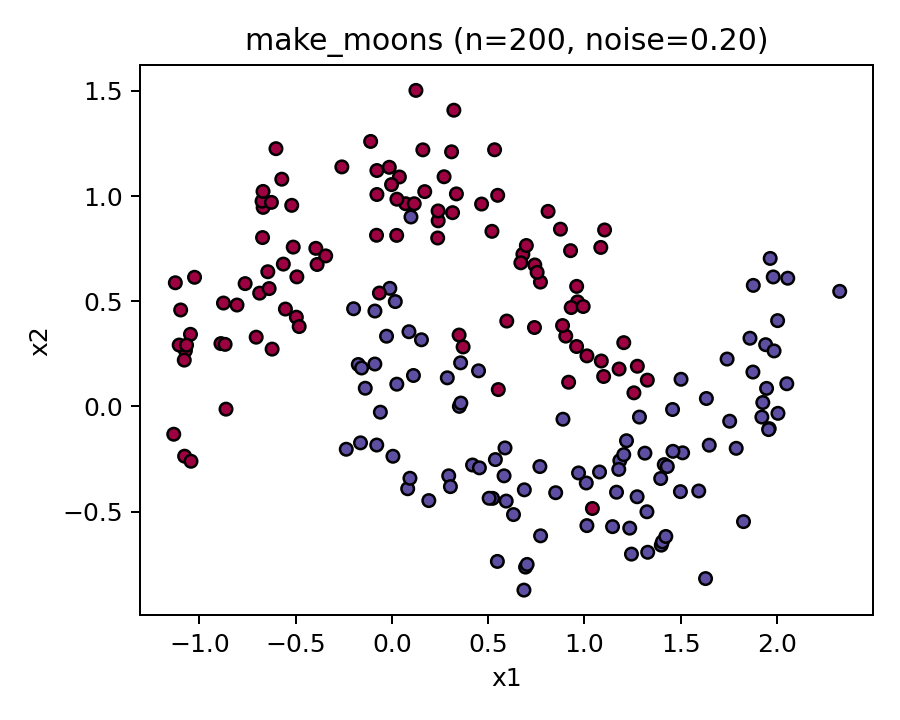
\includegraphics[width=.6\linewidth]{figs/moons_raw.png}}
  \caption{Make-Moons dataset ($n{=}200$, noise $0.20$).}
  \label{fig:moons-scatter}
\end{figure}


\subsection{(b) Activation Functions and Derivatives}
Implemented \(\tanh\), \(\sigma\) (sigmoid), and ReLU activations and their elementwise derivatives:\vspace{.2em}
\begin{align*}
  \tanh(z) &= \frac{e^{z} - e^{-z}}{e^{z} + e^{-z}}, & \tanh'(z) &= 1 - \tanh^2(z),\\
  \sigma(z) &= \frac{1}{1+e^{-z}}, & \sigma'(z) &= \sigma(z)\bigl(1-\sigma(z)\bigr),\\
  \mathrm{ReLU}(z) &= \max(0,z), & \mathrm{ReLU}'(z) &= \mathbf{1}\{z>0\}.
\end{align*}
These functions are exposed as \verb|actFun(z,type)| and \verb|diff_actFun(z,type)| as needed in the file \newline \texttt{three\_layer\_neural\_network.py}.

\subsection{(c) Network and Loss}
Using the notation (page~2, Eq.~(1)--(3)), with \(x\in\mathbb{R}^2\), hidden width \(H\), and \(C=2\) classes:
\begin{align}
z_1 &= x W_1 + b_1, \qquad a_1 = \phi(z_1),\\
z_2 &= a_1 W_2 + b_2, \qquad \hat{y} = \mathrm{softmax}(z_2).
\end{align}
With one-hot \(y\) and probabilities \(\hat{y}\), the average cross-entropy loss (page~3, Eq.~(5)) is
\begin{equation}
  \mathcal{L}(y,\hat{y}) = -\frac{1}{N}\sum_{n=1}^N \sum_{i=1}^C y_{n,i}\log \hat{y}_{n,i}.
\end{equation}
I implemented \verb|feedforward| and \verb|calculate_loss| exactly per the spec.

\subsection{(d) Backpropagation --- Gradients}
For softmax + cross-entropy, the gradient at the output pre-activations is
\(\frac{\partial \mathcal{L}}{\partial z_2} = \frac{1}{N}(\hat{Y}-Y)\).
Then
\begin{align}
\frac{\partial \mathcal{L}}{\partial W_2} &= a_1^\top \frac{\partial \mathcal{L}}{\partial z_2}, &
\frac{\partial \mathcal{L}}{\partial b_2} &= \mathbf{1}^\top \frac{\partial \mathcal{L}}{\partial z_2},\\
\frac{\partial \mathcal{L}}{\partial z_1} &= \Bigl(\frac{\partial \mathcal{L}}{\partial z_2} W_2^\top\Bigr)\odot \phi'(z_1),\\
\frac{\partial \mathcal{L}}{\partial W_1} &= X^\top \frac{\partial \mathcal{L}}{\partial z_1}, &
\frac{\partial \mathcal{L}}{\partial b_1} &= \mathbf{1}^\top \frac{\partial \mathcal{L}}{\partial z_1}.
\end{align}
These are implemented in \verb|backprop| and used with vanilla SGD updates.

\subsection{(e) Training and Decision Boundaries}
I trained the model with each activation (Tanh, Sigmoid, ReLU) and saved decision-boundary plots. The tanh network stays smooth yet zero-centered, letting \(H{=}3\) bend around the moons without skewing the decision surface. Sigmoid units saturate near 0 and 1, so the boundary flattens at the extremes and cannot wrap as tightly around the inner moon. ReLU partitions the plane into straight wedges, yielding sharper corners but leaving a few jagged transitions between classes. In this shallow regime tanh consistently held the lowest error because it remains expressive without fully saturating.
\begin{figure}[H]
\centering
\begin{tabular}{ccc}
\fbox{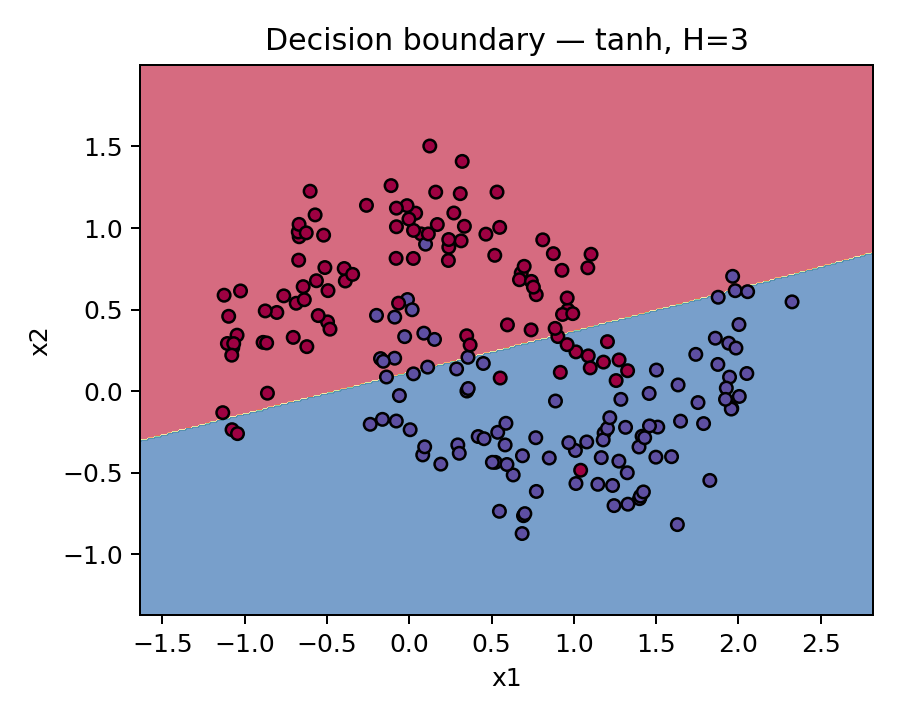
\includegraphics[width=.29\linewidth]{figs/decision_boundary_tanh_H3.png}} &
\fbox{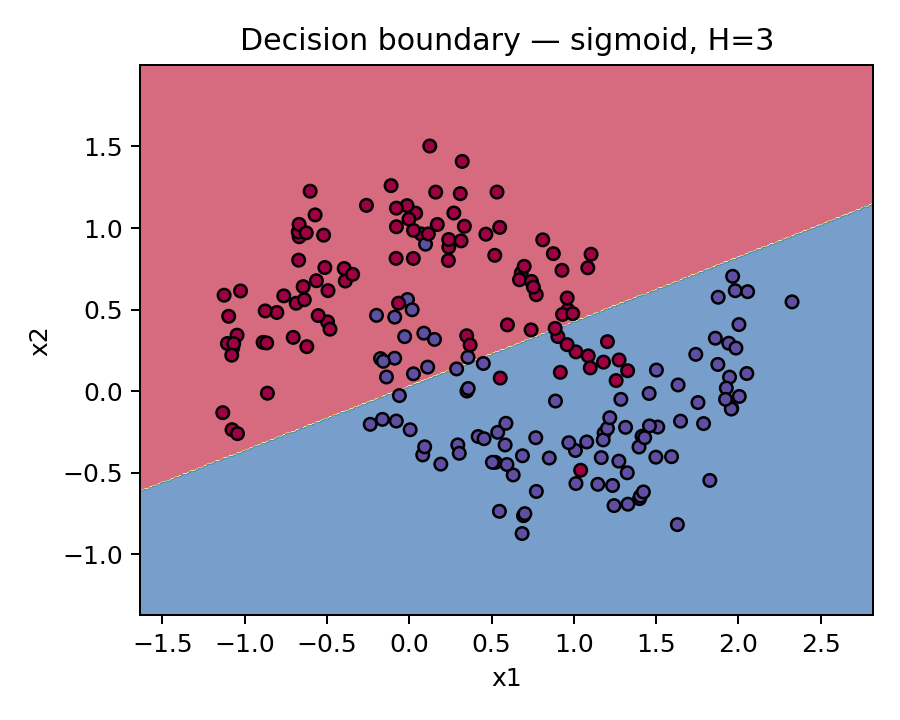
\includegraphics[width=.29\linewidth]{figs/decision_boundary_sigmoid_H3.png}} &
\fbox{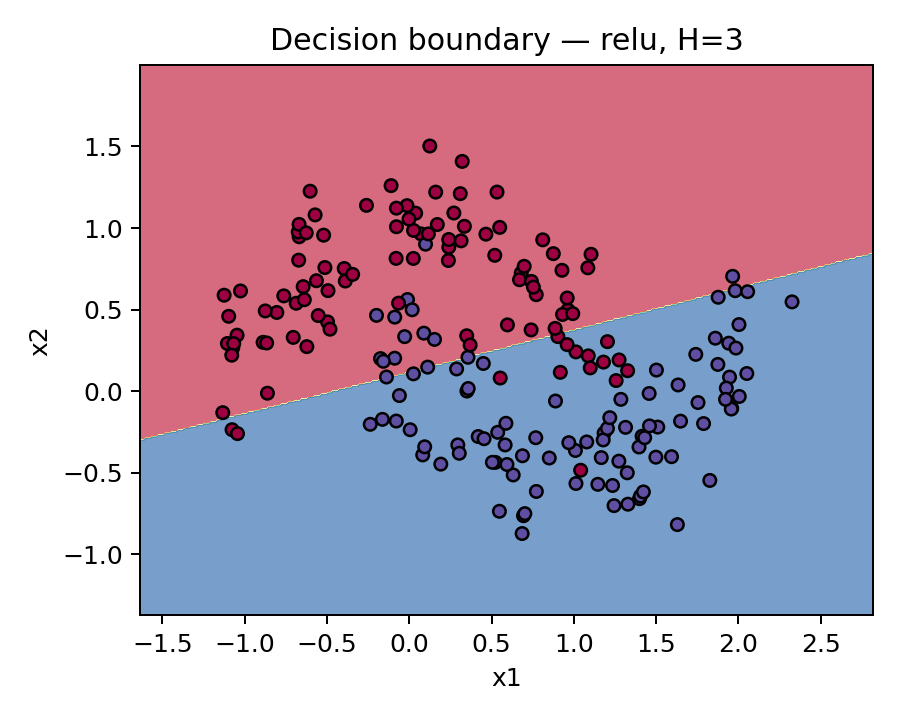
\includegraphics[width=.29\linewidth]{figs/decision_boundary_relu_H3.png}}\\
Tanh ($H$=3) & Sigmoid ($H$=3) & ReLU ($H$=3)
\end{tabular}
\caption{Decision boundaries across activations.}
\end{figure}

\noindent Next, I increased the hidden width \(H\in\{3,10,50\}\) (Tanh). The saved decision boundaries illustrate how capacity changes the fit:
\begin{figure}[H]
\centering
\begin{tabular}{ccc}
\fbox{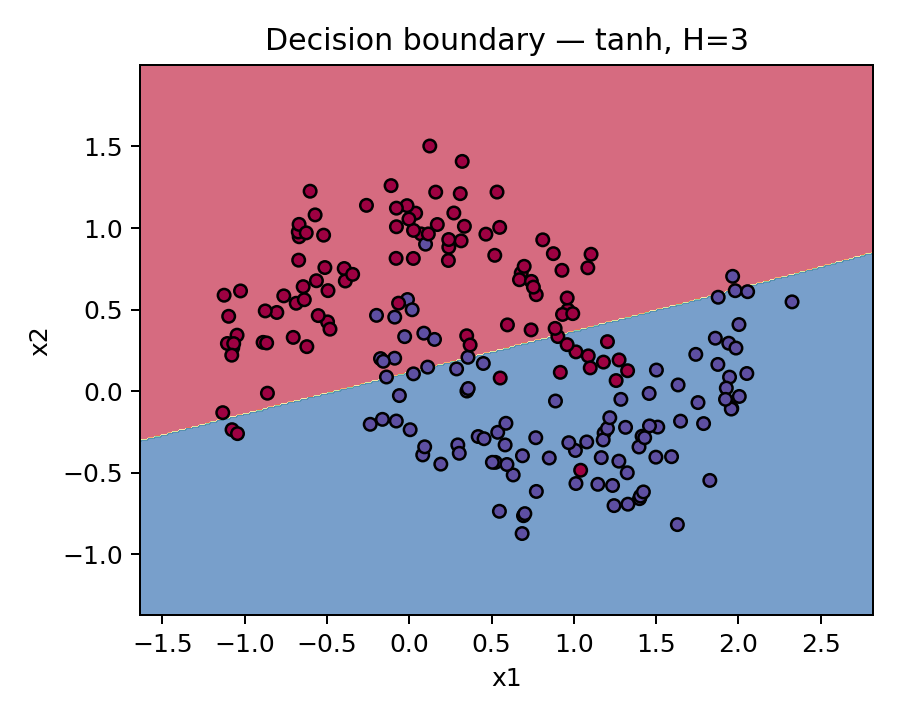
\includegraphics[width=.29\linewidth]{figs/decision_boundary_tanh_H3.png}} &
\fbox{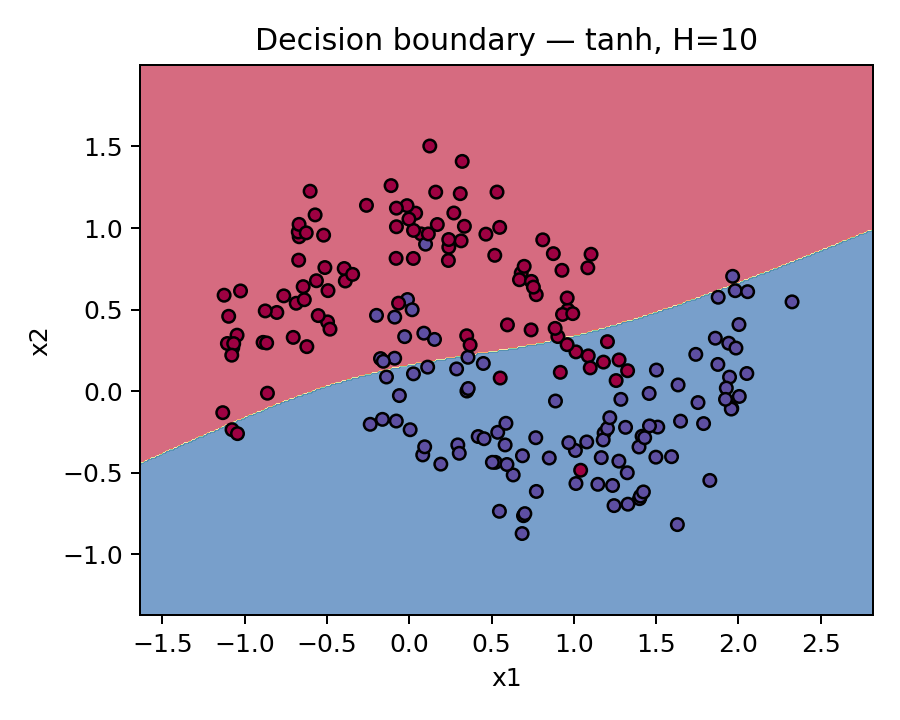
\includegraphics[width=.29\linewidth]{figs/decision_boundary_tanh_H10.png}} &
\fbox{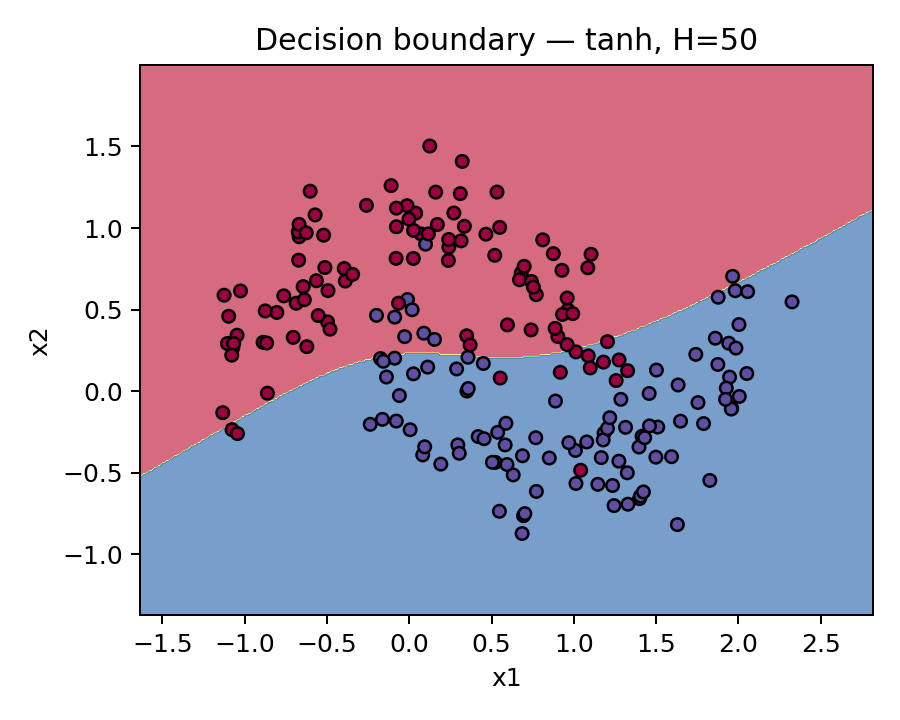
\includegraphics[width=.29\linewidth]{figs/decision_boundary_tanh_H50.png}}\\
Tanh ($H$=3) & Tanh ($H$=10) & Tanh ($H$=50)
\end{tabular}
\caption{Decision boundaries as hidden width increases (Tanh). Larger $H$ yields higher capacity and more intricate boundaries.}
\end{figure}

\newpage

\subsection{(f) Deeper Network}
I implemented a general \(n\)-layer MLP in \texttt{n\_layer\_neural\_network.py} that accepts the number of hidden layers and layer size as parameters, and adds L2 weight regularization to the loss. The implementation uses lists \(\{W^\ell,b^\ell\}_{\ell=1}^L\), supports \(\{\mathrm{ReLU},\tanh,\sigma\}\), and performs full backprop with softmax output. \newline \newline
\noindent I trained on Make-Moons with several depths and widths, then repeated on two other toy datasets (\texttt{make\_circles} and \texttt{make\_blobs}).
The circles dataset contains two concentric rings that are not linearly separable, so additional depth lets stacked nonlinearities carve out the hollow annulus while extra width sharpens the inner boundary. The blobs dataset instead has roughly spherical clusters that are almost linearly separable; shallow nets already perform well, and wider layers mainly warp the margin to match each cluster's covariance. Comparing the two highlighted how geometry drives architectural needs: depth helps capture curved wraps on circles, whereas blobs mostly test whether the model can keep a stable, near-linear cut.
\begin{figure}[H]
\centering
\begin{tabular}{ccc}
\fbox{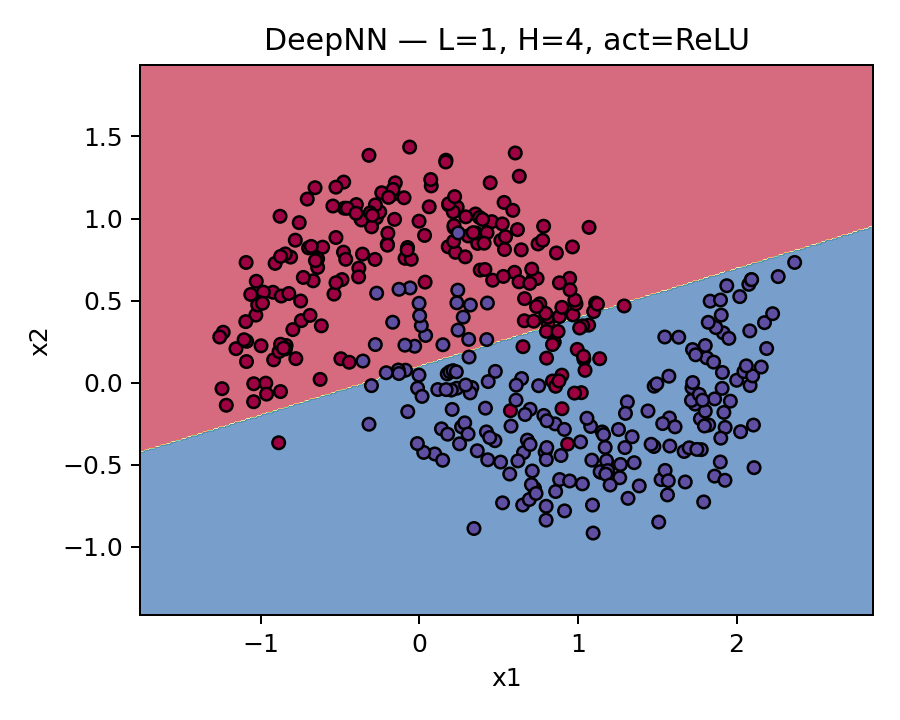
\includegraphics[width=.29\linewidth]{figs/deep_decision_L1_H4.png}} &
\fbox{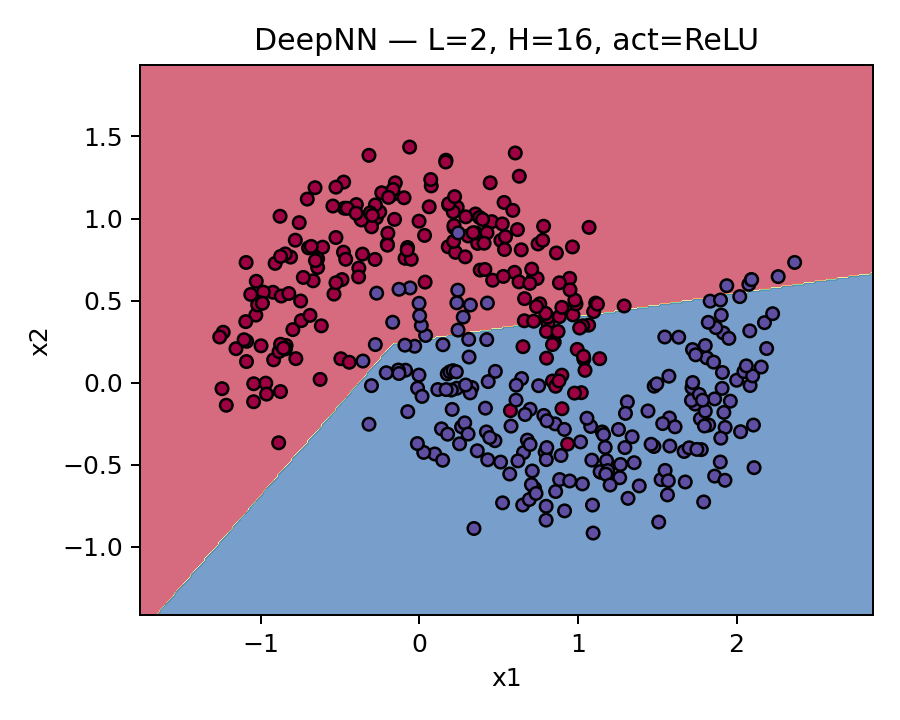
\includegraphics[width=.29\linewidth]{figs/deep_decision_L2_H16.png}} &
\fbox{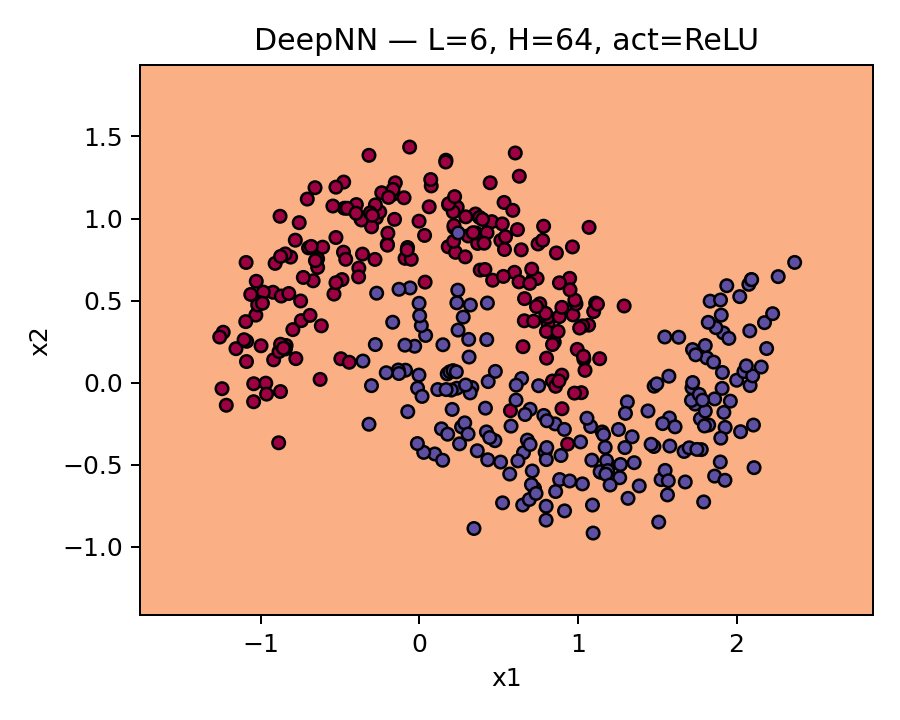
\includegraphics[width=.29\linewidth]{figs/deep_decision_L6_H64.png}}\\
$L{=}1, H{=}4$ & $L{=}2, H{=}16$ & $L{=}6, H{=}64$
\end{tabular}
\caption{Representative decision boundaries for the $n$-layer MLP on Make-Moons as depth ($L$) and width ($H$) vary.}
\end{figure}

\begin{figure}[H]
\centering
\begin{tabular}{cc}
\fbox{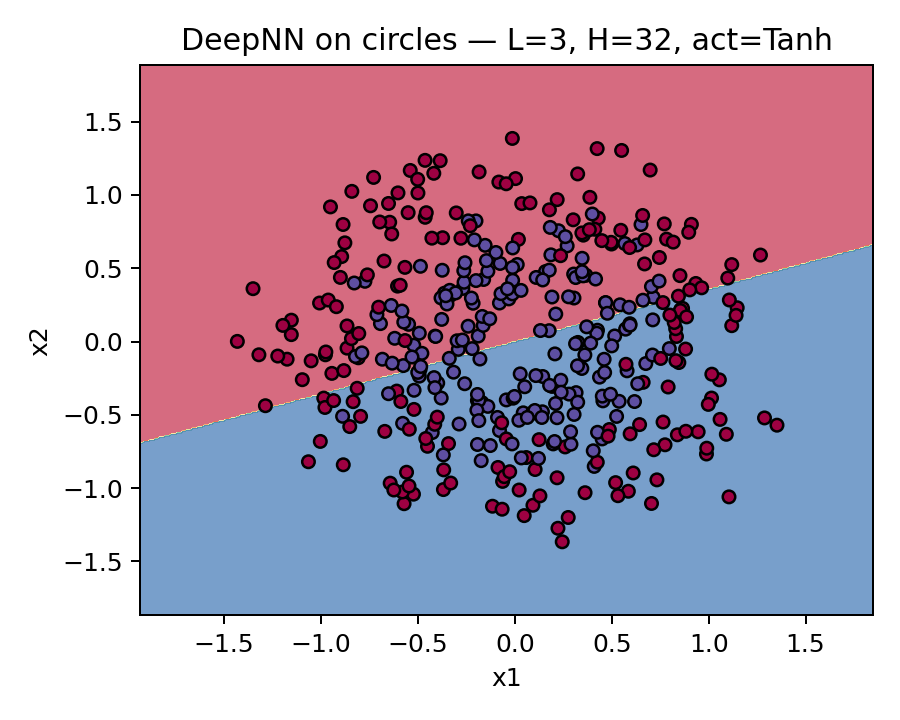
\includegraphics[width=.4\linewidth]{figs/deep_circles_L3_H32.png}} &
\fbox{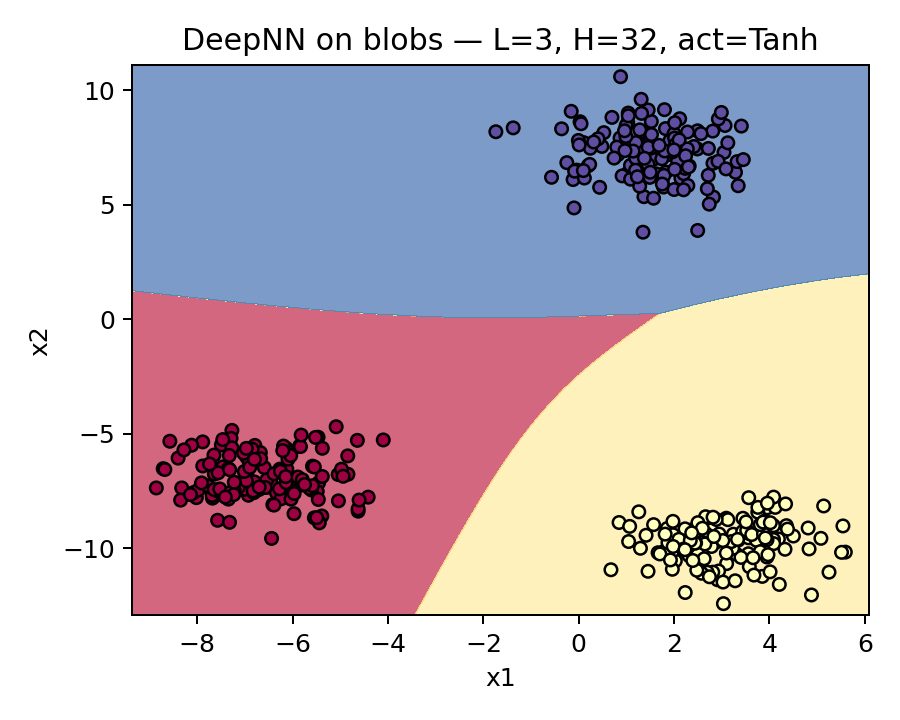
\includegraphics[width=.4\linewidth]{figs/deep_blobs_L3_H32.png}}\\
Circles ($L{=}3, H{=}32$, Tanh) & Blobs ($L{=}3, H{=}32$, Tanh)
\end{tabular}
\caption{Generalization of the deeper MLP to other toy datasets.}
\end{figure}


\paragraph{Design choices (why):}
\begin{itemize}[leftmargin=1.2em]
  \item \textbf{Stable softmax} and \textbf{averaged cross-entropy}: for numerical stability and scale-free gradients.
  \item \textbf{Explicit caches} \(\{z^\ell,a^\ell\}\): simplifies backprop code and matches the math.
  \item \textbf{L2 regularization} in the deeper net: requested in the handout and helps control overfitting on simple datasets.
  \item \textbf{Deterministic seeds}: to reproduce plots across runs.
\end{itemize}

\newpage

\section{Part 2 --- Simple DCN on MNIST}
\subsection{(a) Build and Train a 4-layer DCN}
The architecture has been built according to the required form: \texttt{conv1(5-5-1-32) - ReLU - maxpool(2-2) - conv2(5-5-32-64) - ReLU - maxpool(2-2) - fc(1024) - ReLU - DropOut(0.5) - Softmax(10)}. The code uses \texttt{CrossEntropyLoss}, which combines \texttt{log-softmax} and NLL, so the network returns logits; probabilities are only needed for inspection. I split 55k/5k for train/val and report test accuracy. TensorBoard logs the training loss.

\paragraph{Reported accuracy: 0.9888 } 

\subsection{(b) Visualizing Training in More Detail}
Per the instructions, I monitor, every 100 iterations: (1) \emph{weights and biases} (histograms \& summary stats), (2) \emph{pre-activations} \(z\) at each layer, (3) \emph{post-ReLU activations}, and (4) \emph{post-MaxPool activations}. I also log validation and test accuracy once per epoch (approximately every 1100 iterations when using batch size 50 as suggested in the PDF). TensorBoard screenshots should be pasted here after running:

\begin{figure}[H]
\centering
\begin{tabular}{cc}
\fbox{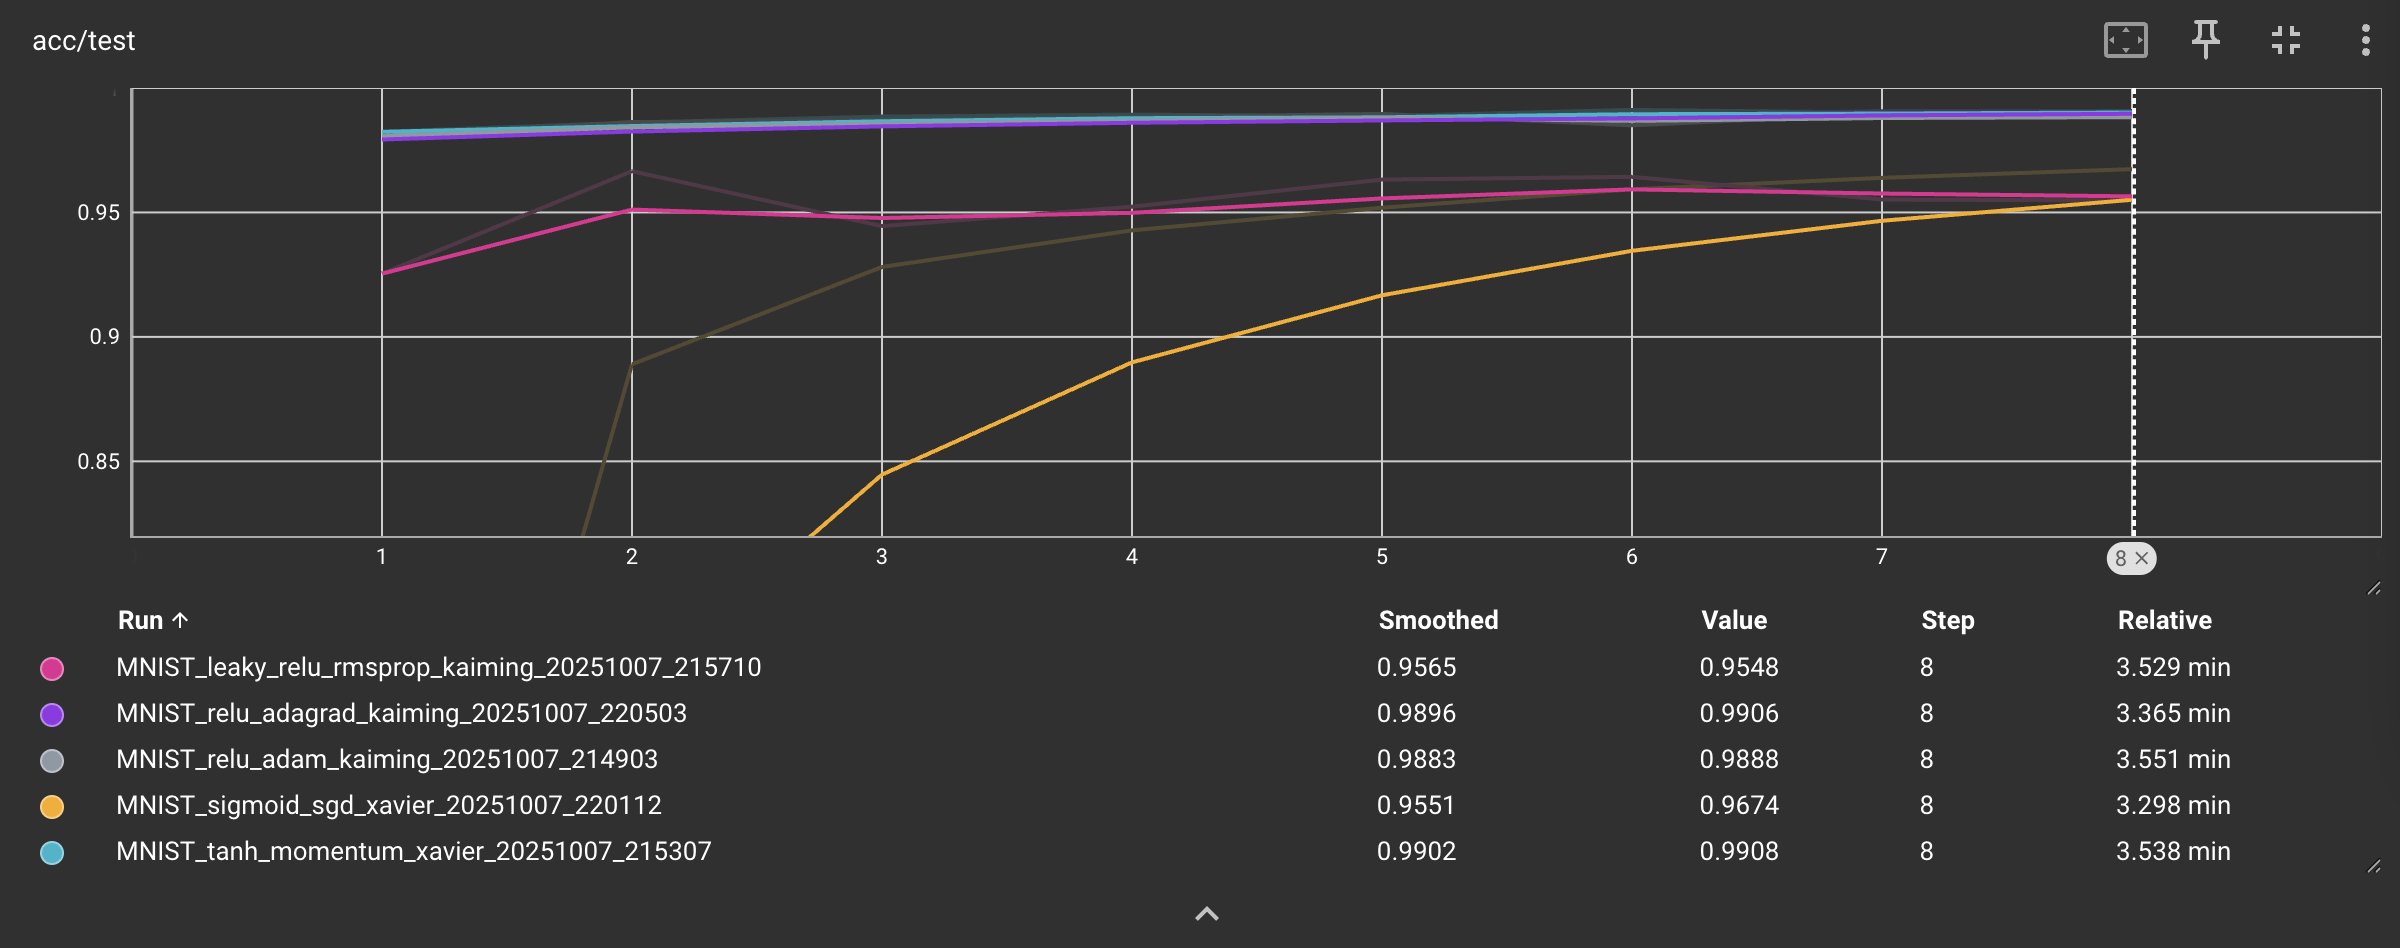
\includegraphics[width=.45\linewidth]{figs/tb_testacc.png}} &
\fbox{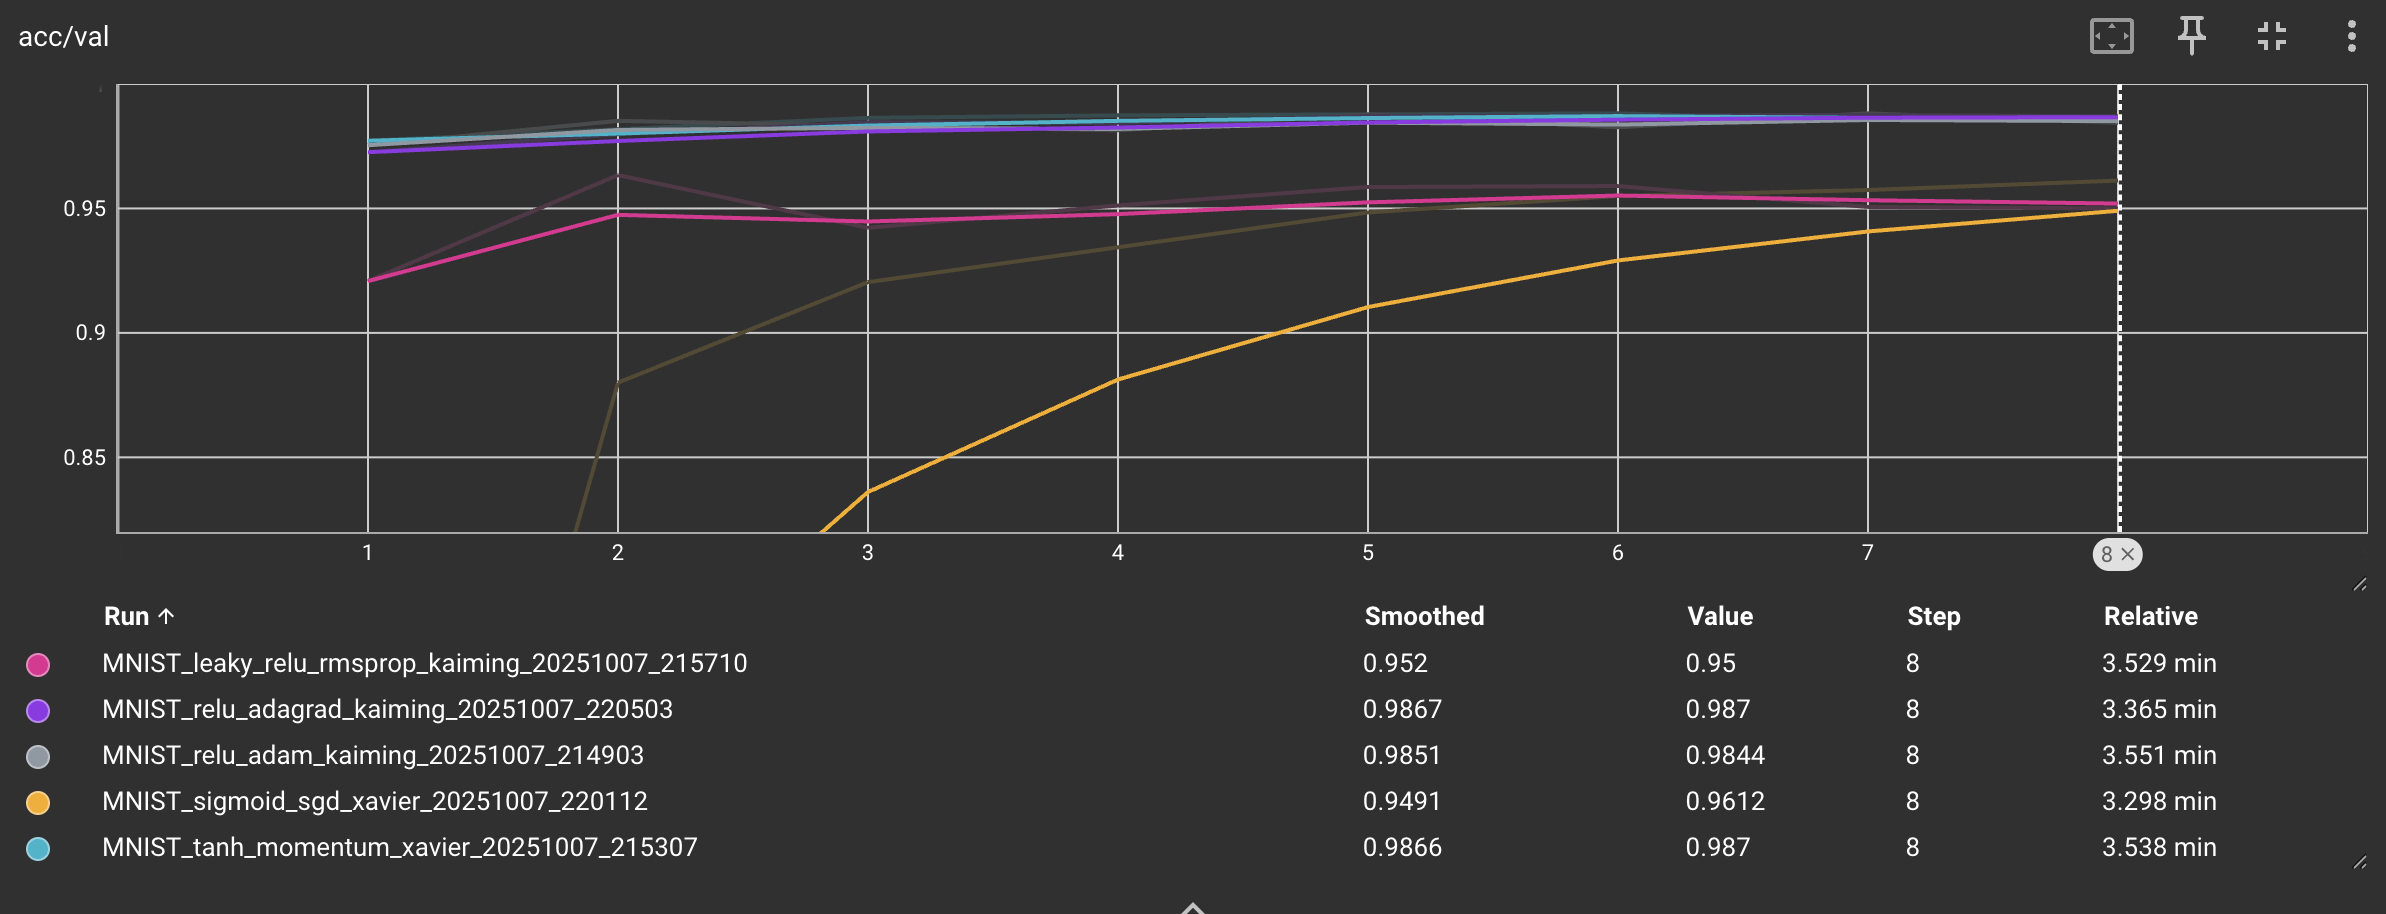
\includegraphics[width=.45\linewidth]{figs/tb_valacc.png}}\\
Test accuracy & Validation accuracy
\end{tabular}

\begin{tabular}{ccc}
\fbox{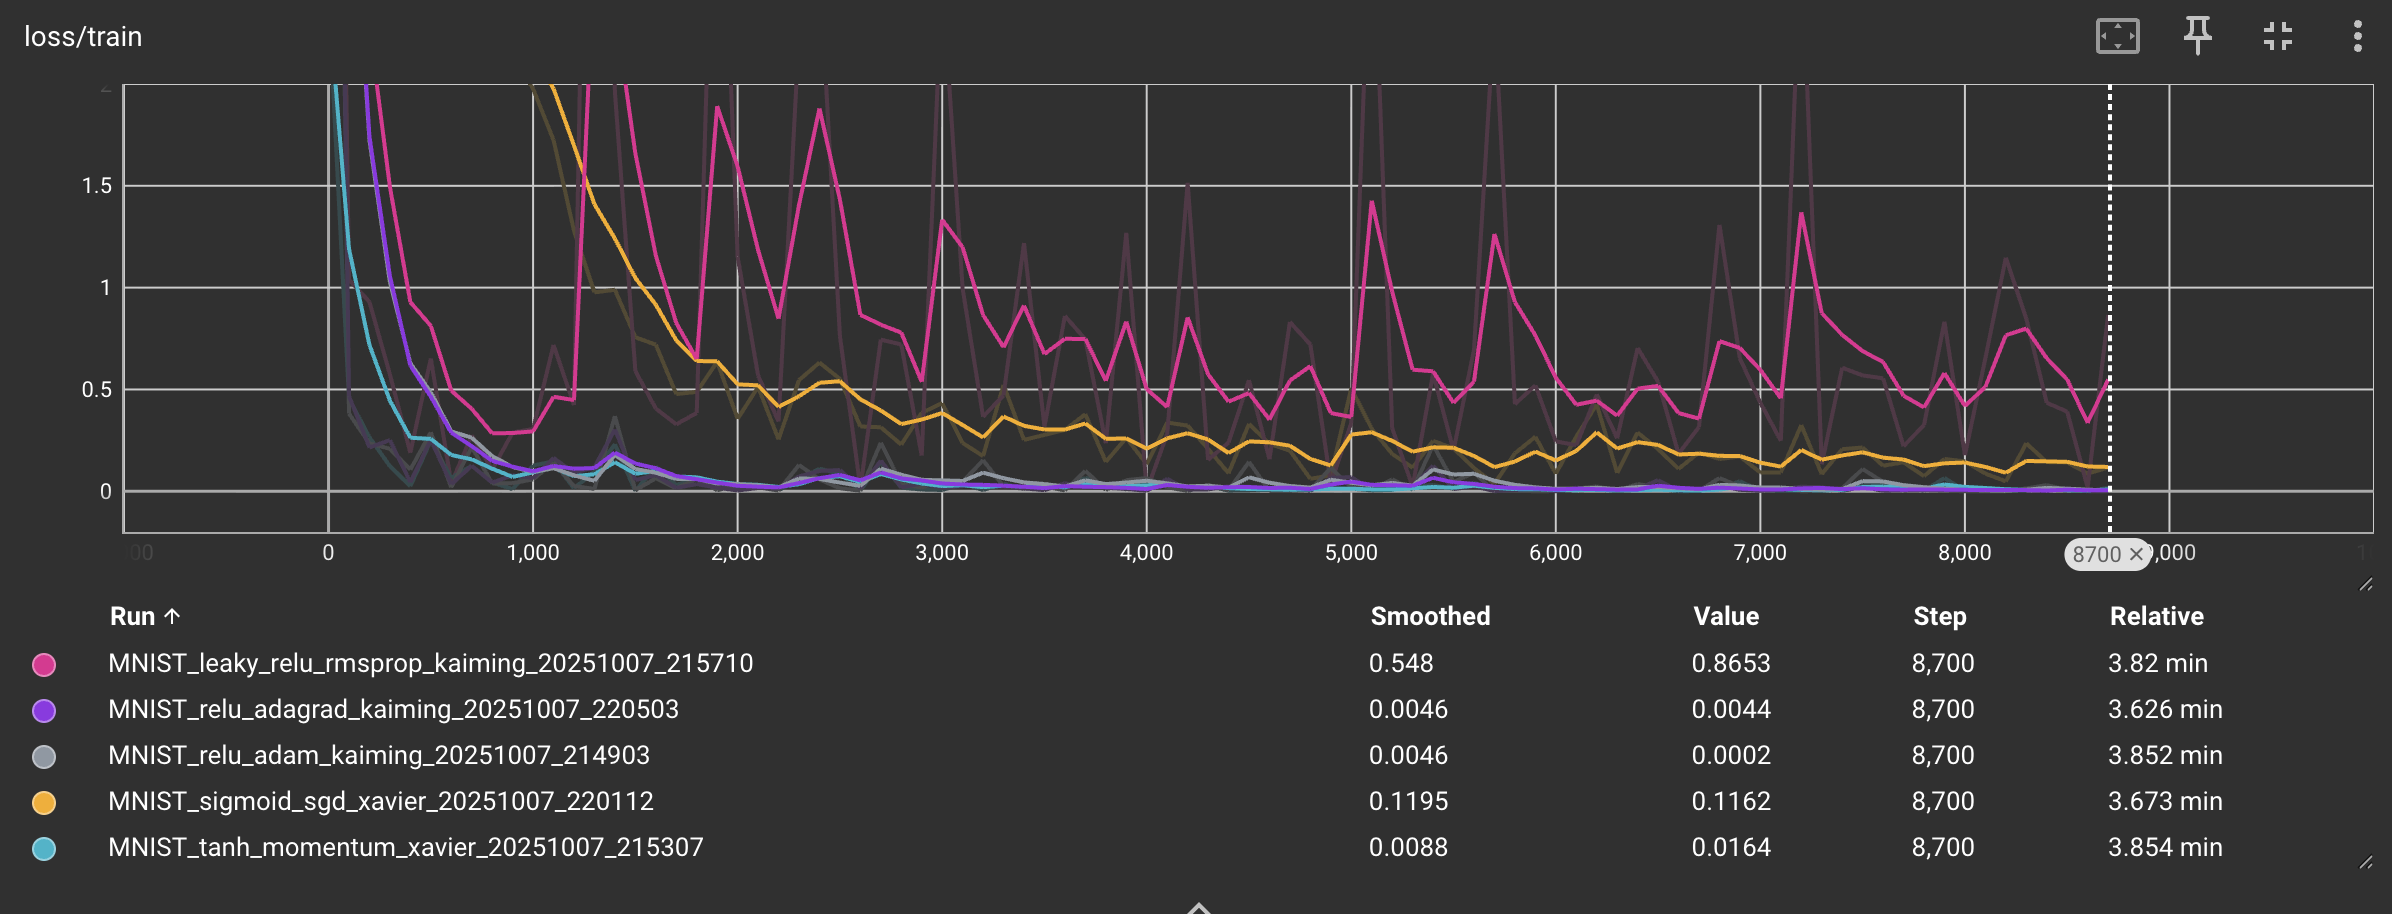
\includegraphics[width=.29\linewidth]{figs/tb_loss.png}} &
\fbox{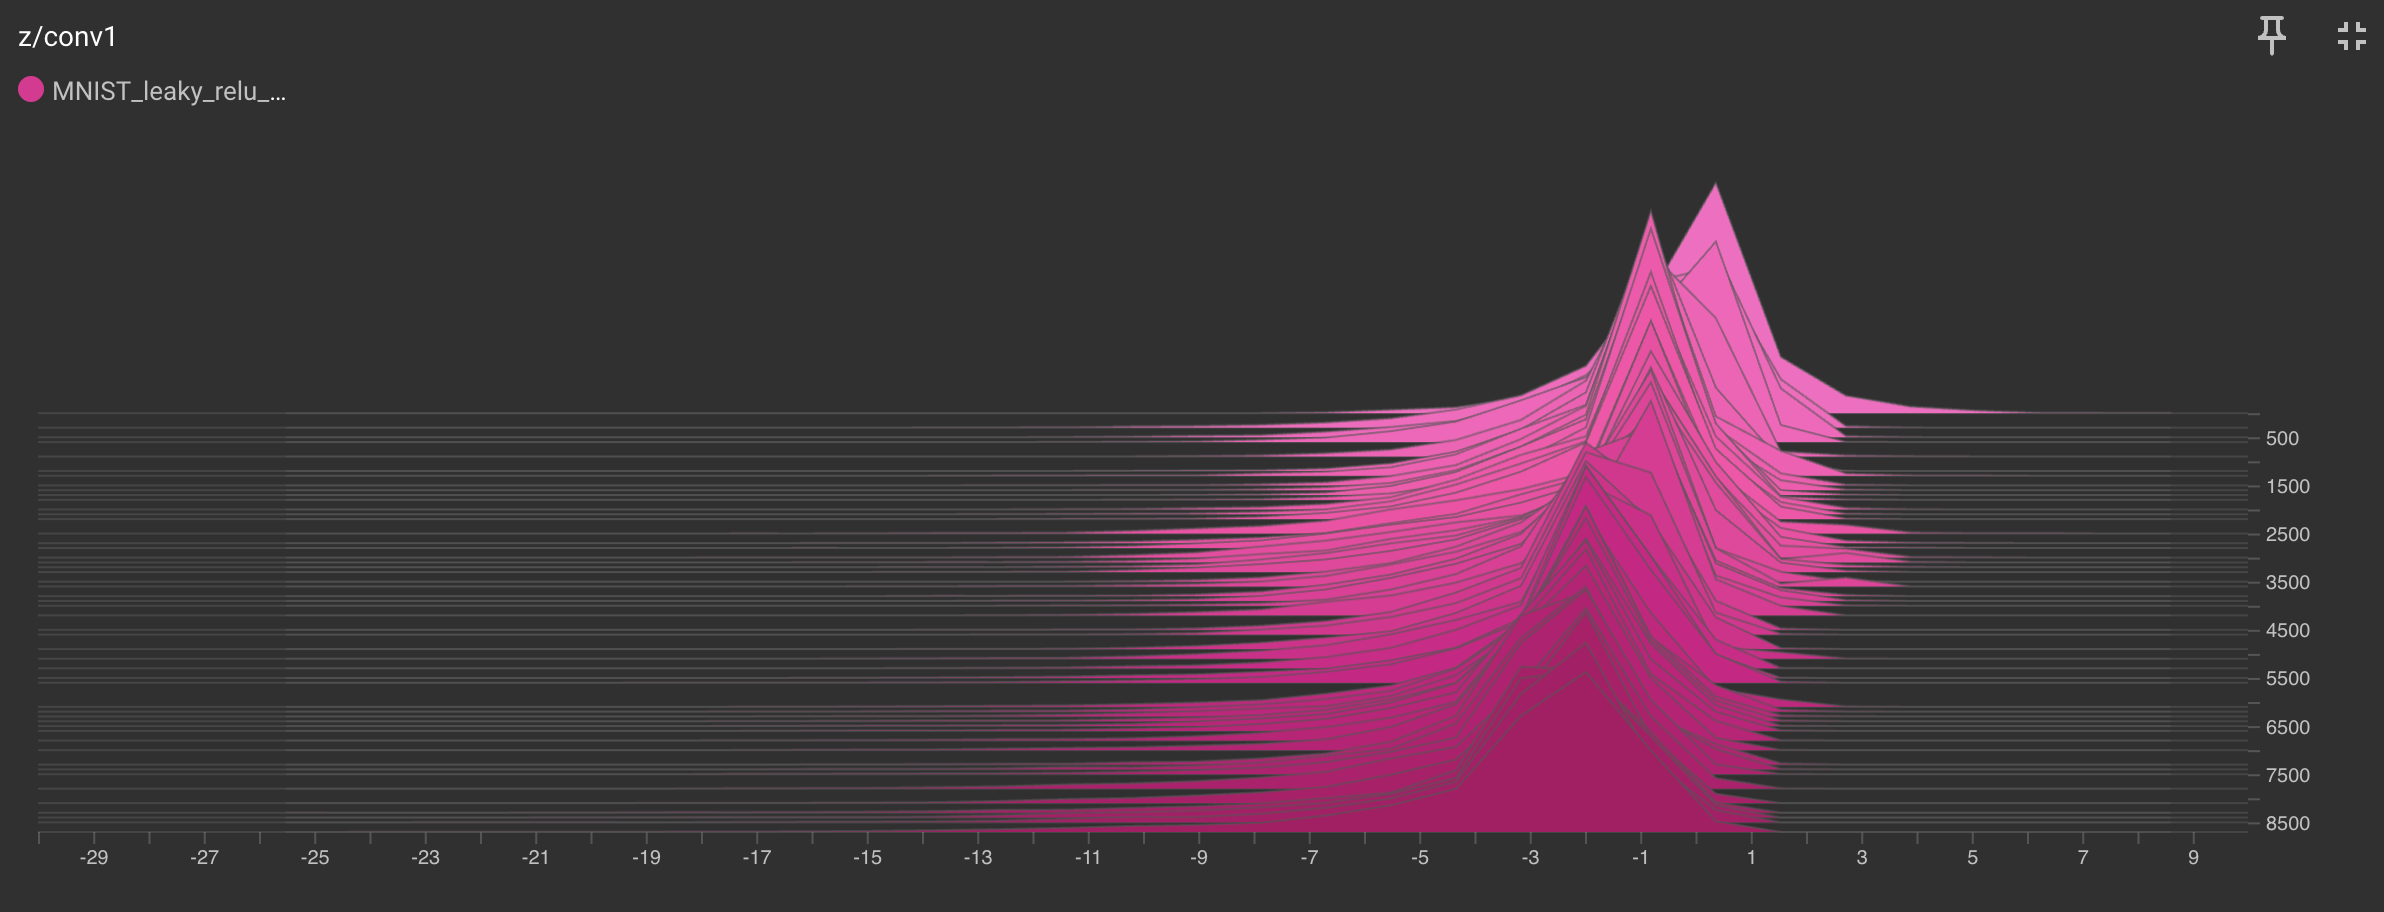
\includegraphics[width=.29\linewidth]{figs/tb_z_conv1_hist.png}} &
\fbox{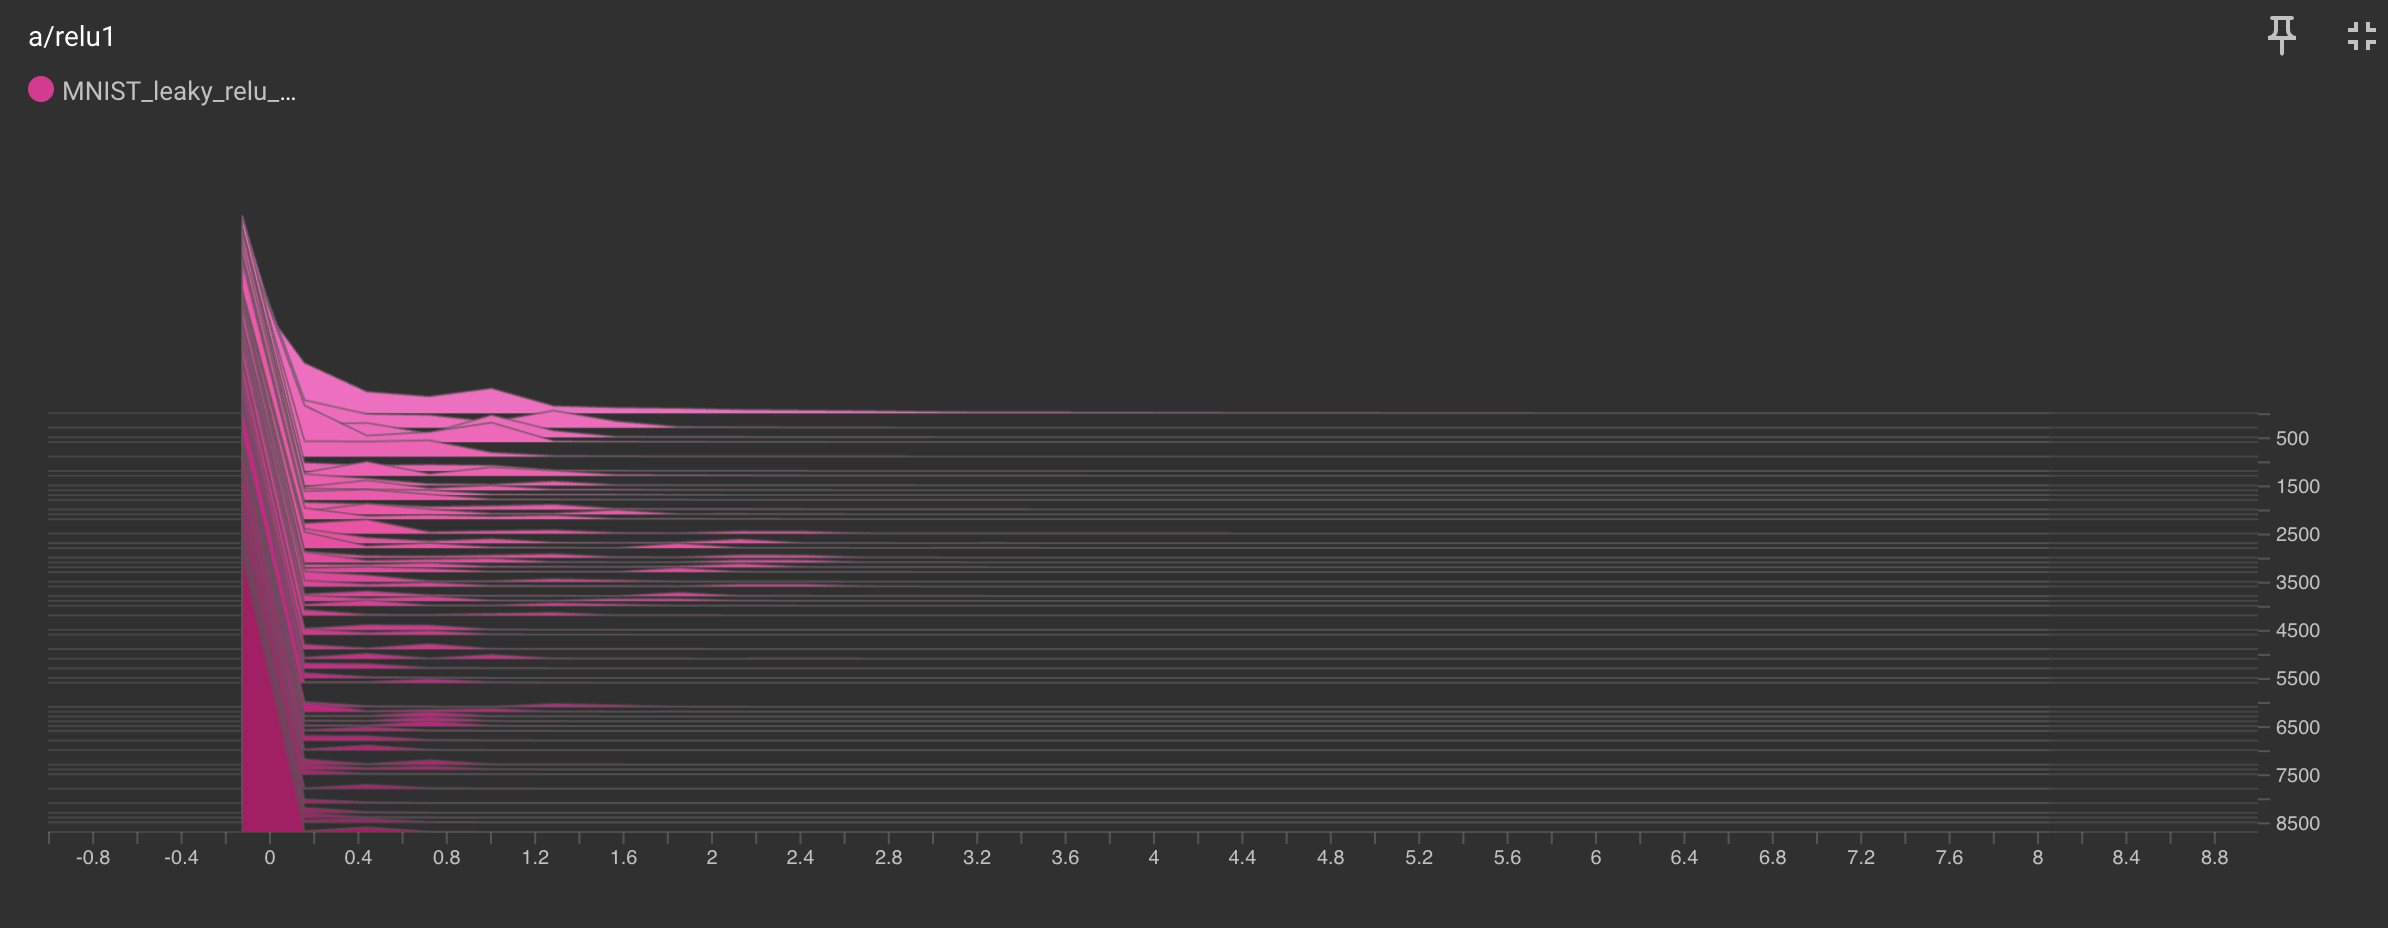
\includegraphics[width=.29\linewidth]{figs/tb_a_relu1_hist.png}}\\
Training loss & Preactivations $z$ (conv1) & Activations (ReLU1)
\end{tabular}

\begin{tabular}{cc}
\fbox{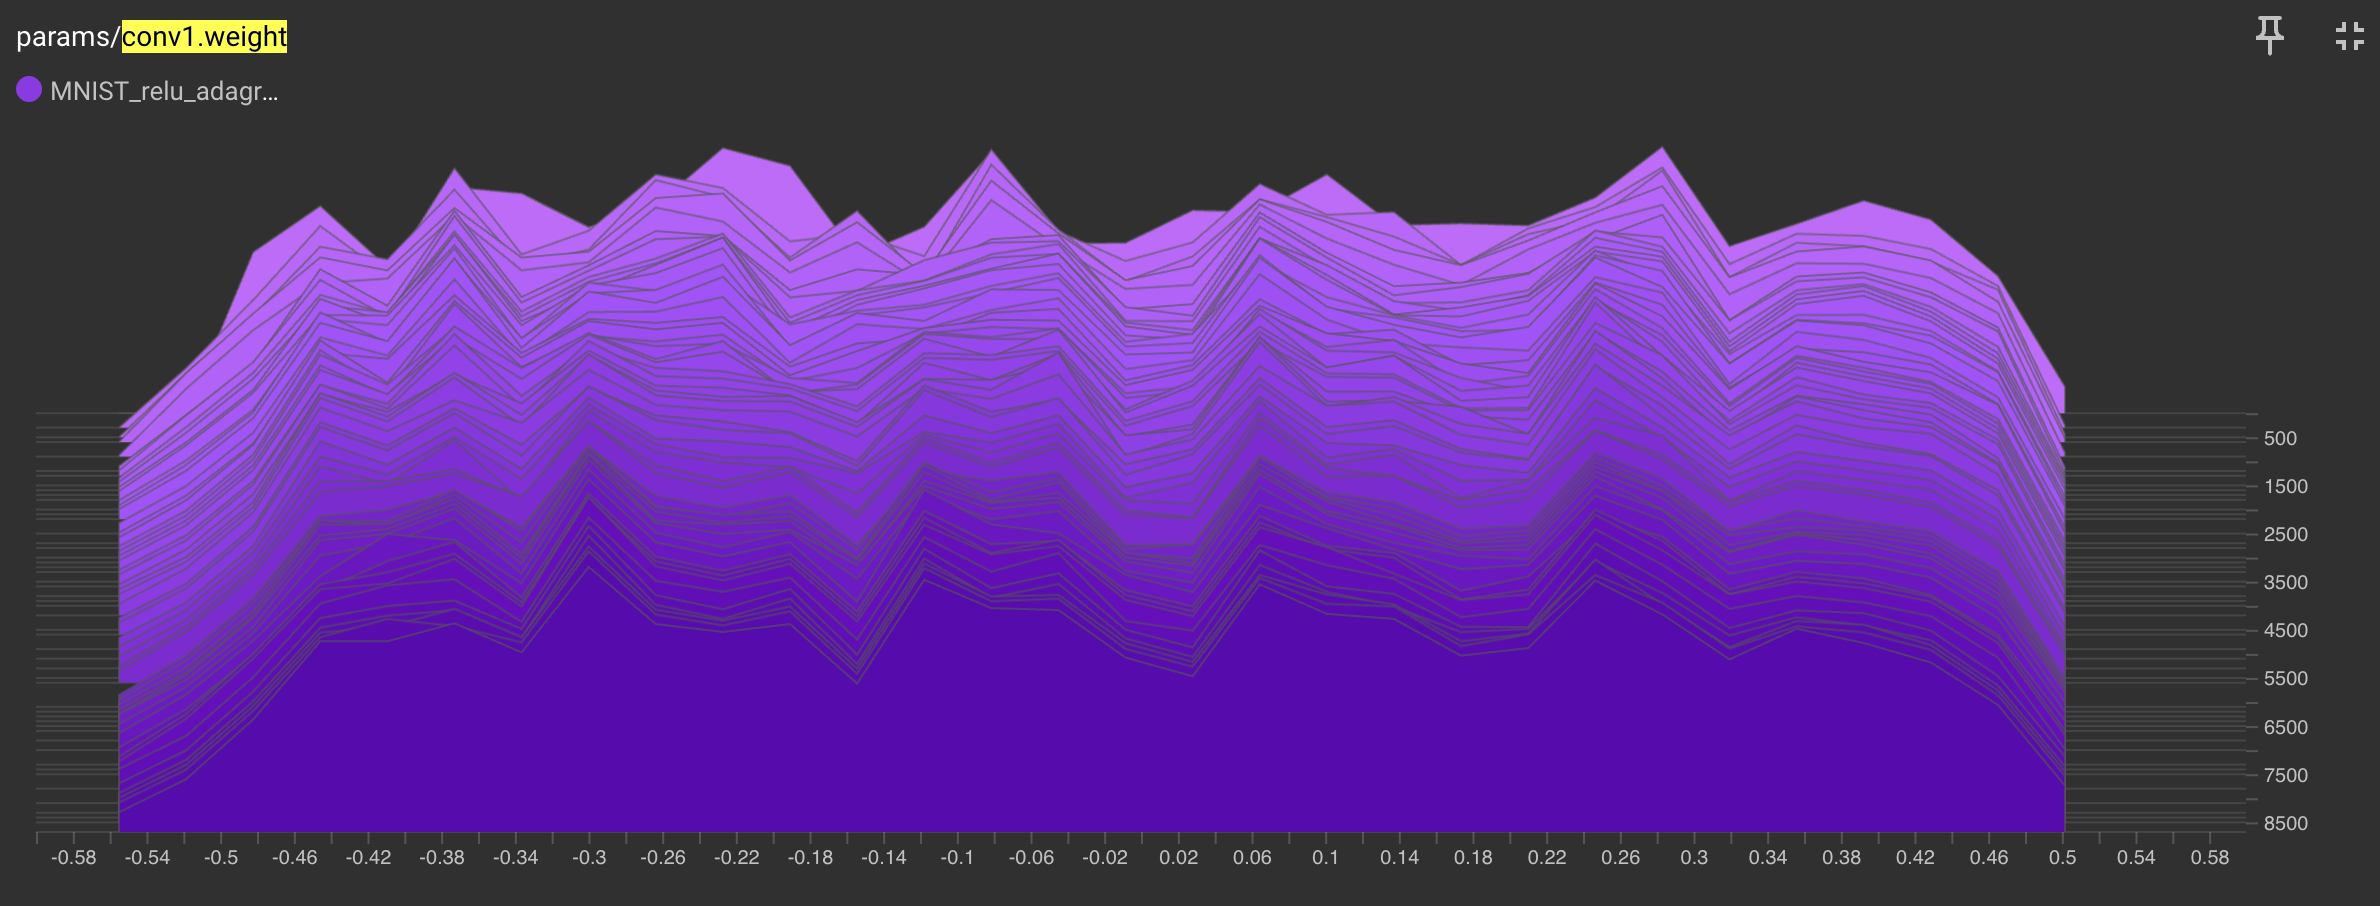
\includegraphics[width=.29\linewidth]{figs/tb_params_conv1_weight_hist.png}} &
\fbox{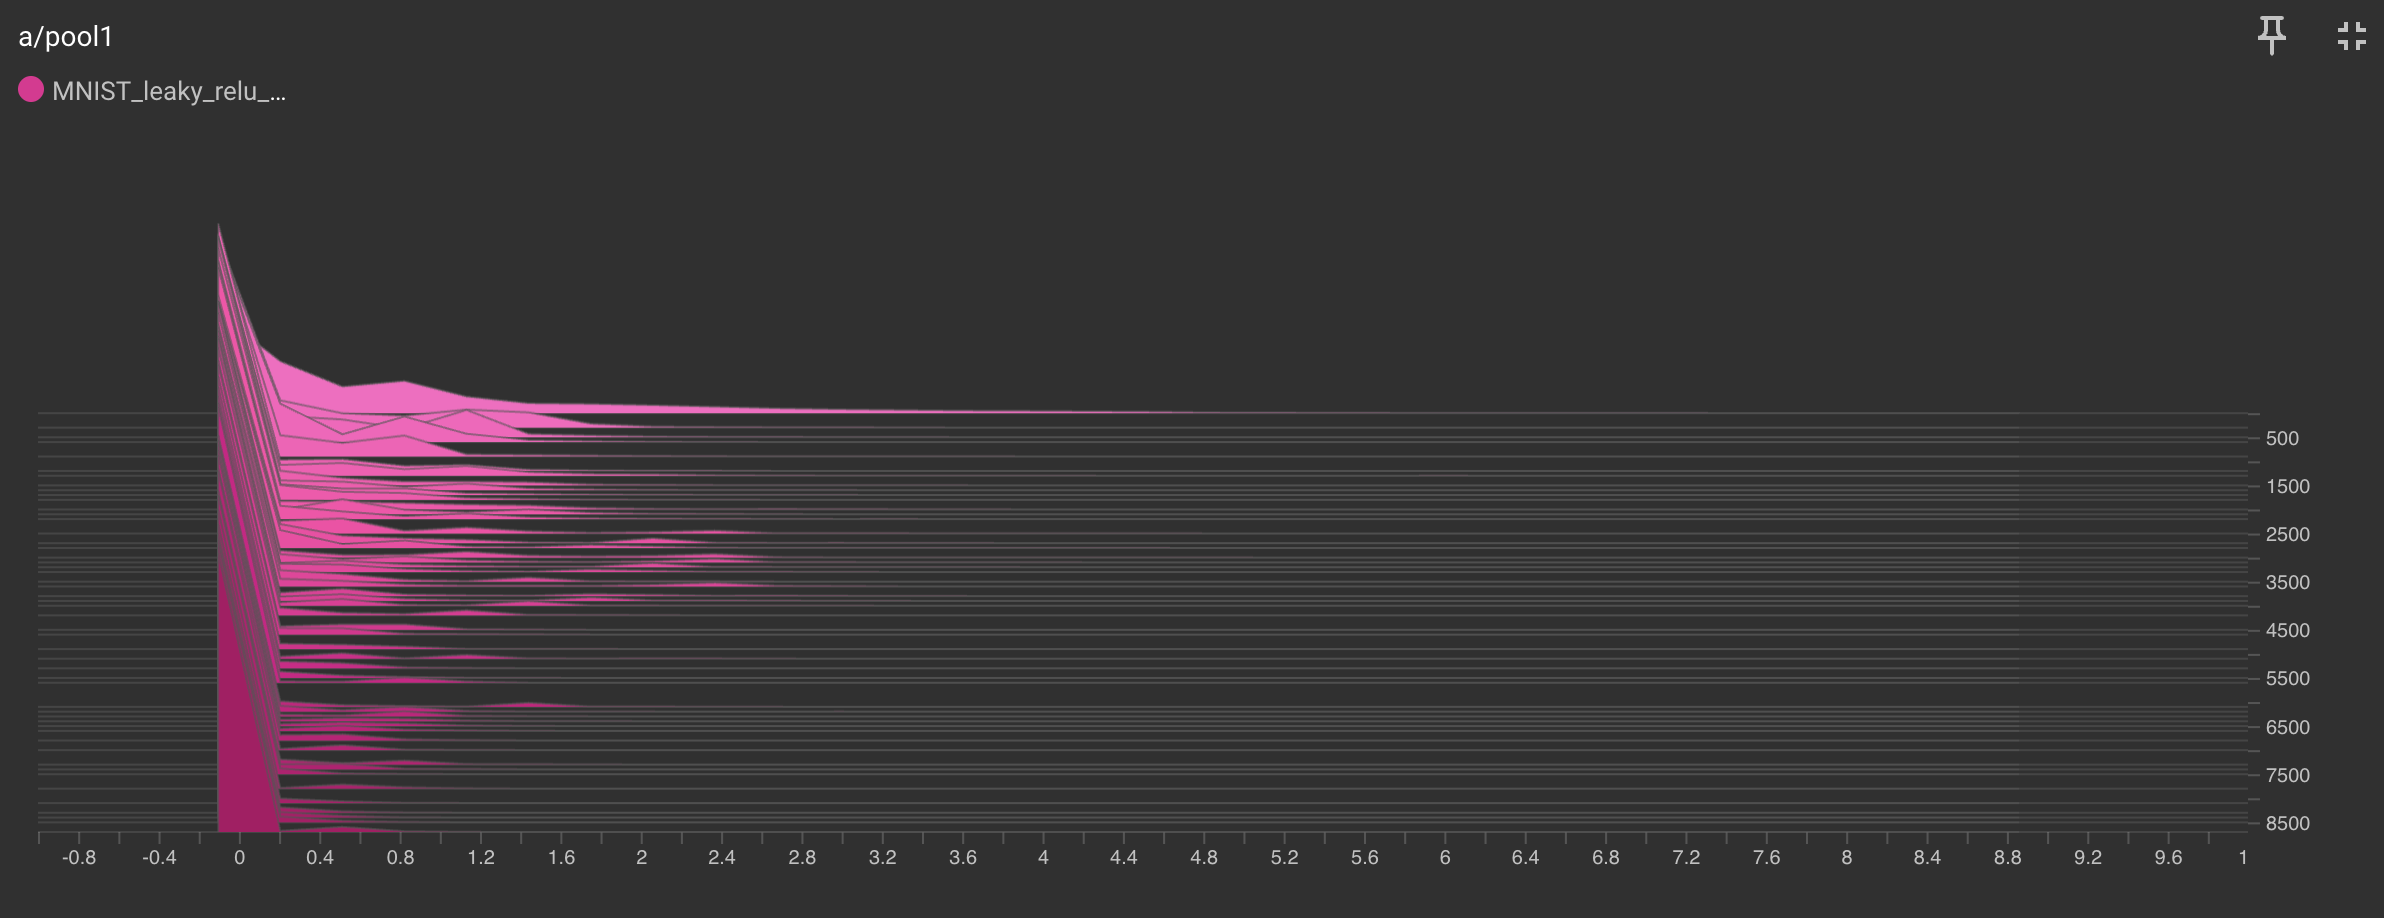
\includegraphics[width=.29\linewidth]{figs/tb_a_pool1_hist.png}}\\
Weights (conv1) & Post-MaxPool activations (pool1)
\end{tabular}
\caption{TensorBoard monitoring: loss/accuracy, parameter histograms, and layerwise (pre)activations.}
\end{figure}


\begin{figure}[H]
\centering

% Weights (conv1): min/max/mean/std
\begin{tabular}{cccc}
\fbox{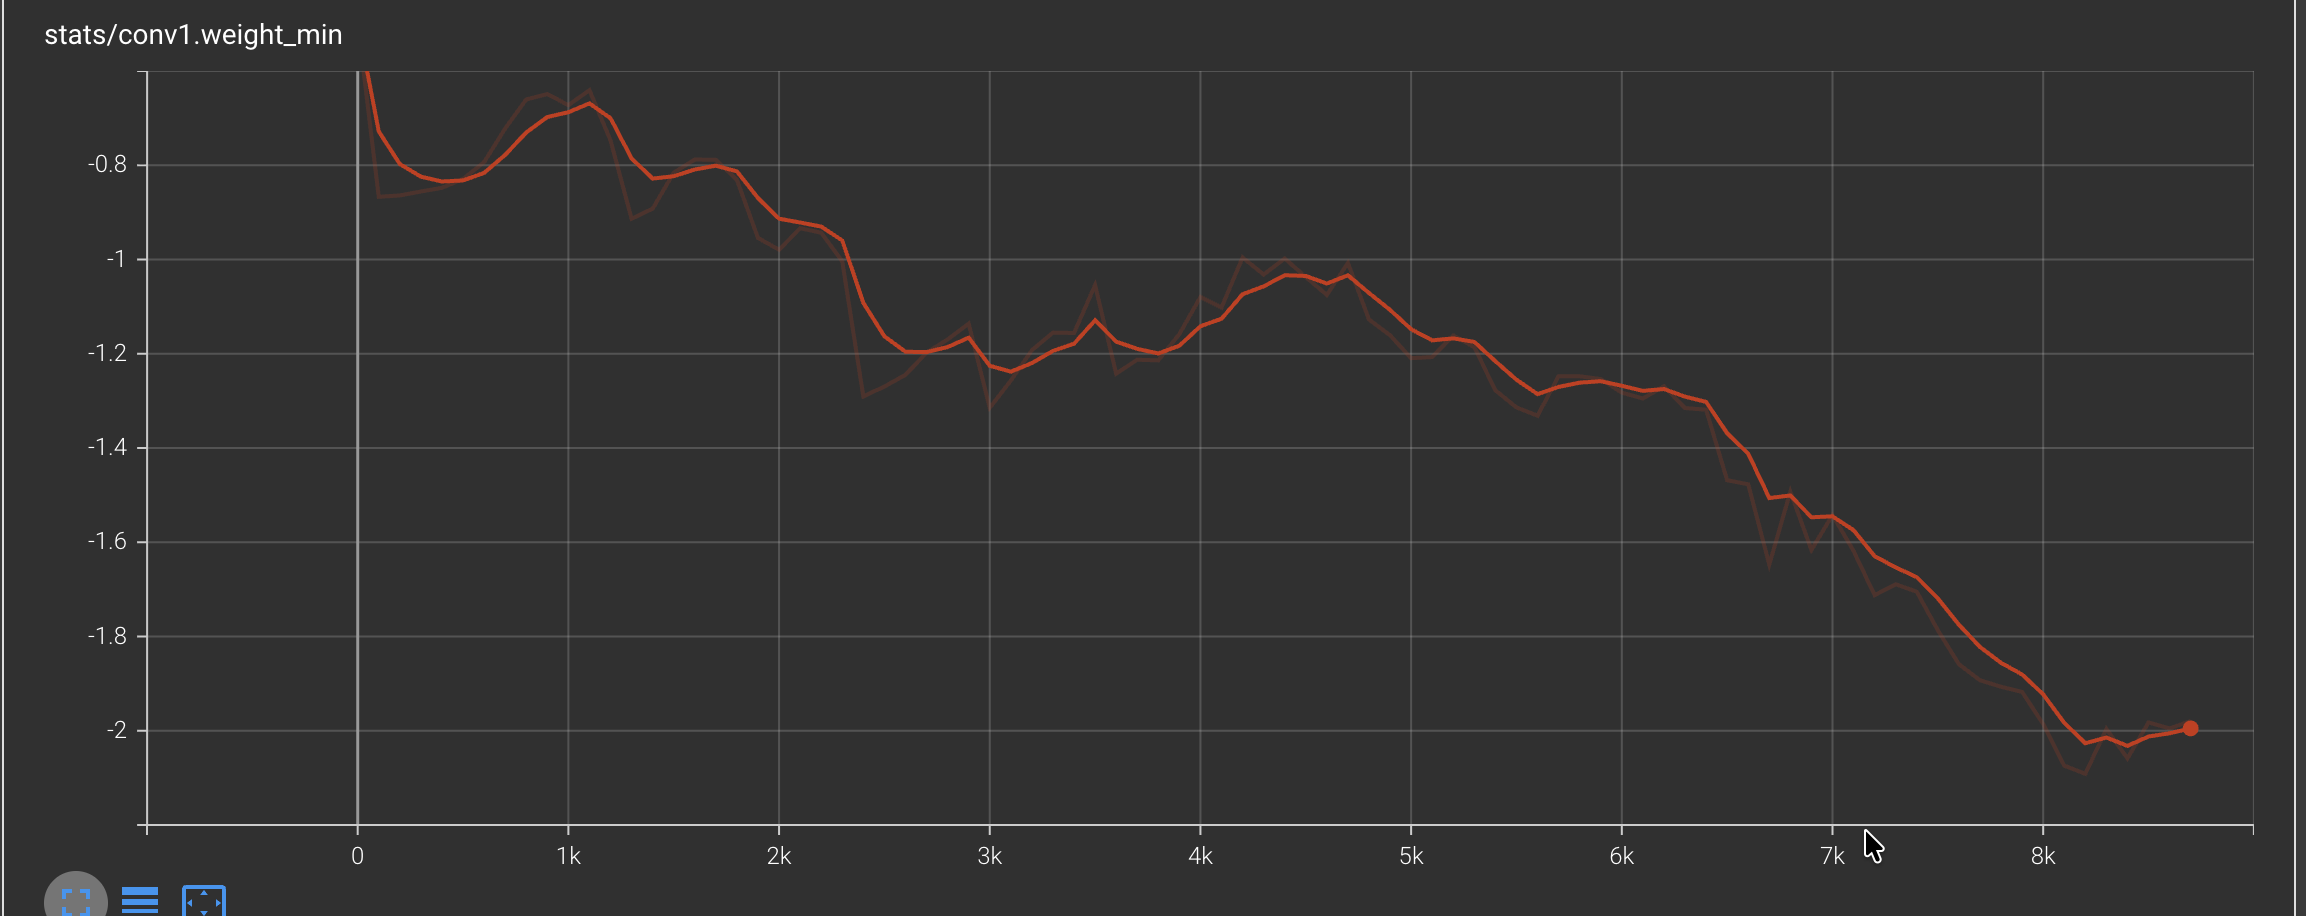
\includegraphics[width=.20\linewidth]{figs/tb_stats_params_conv1_weight_min.png}} &
\fbox{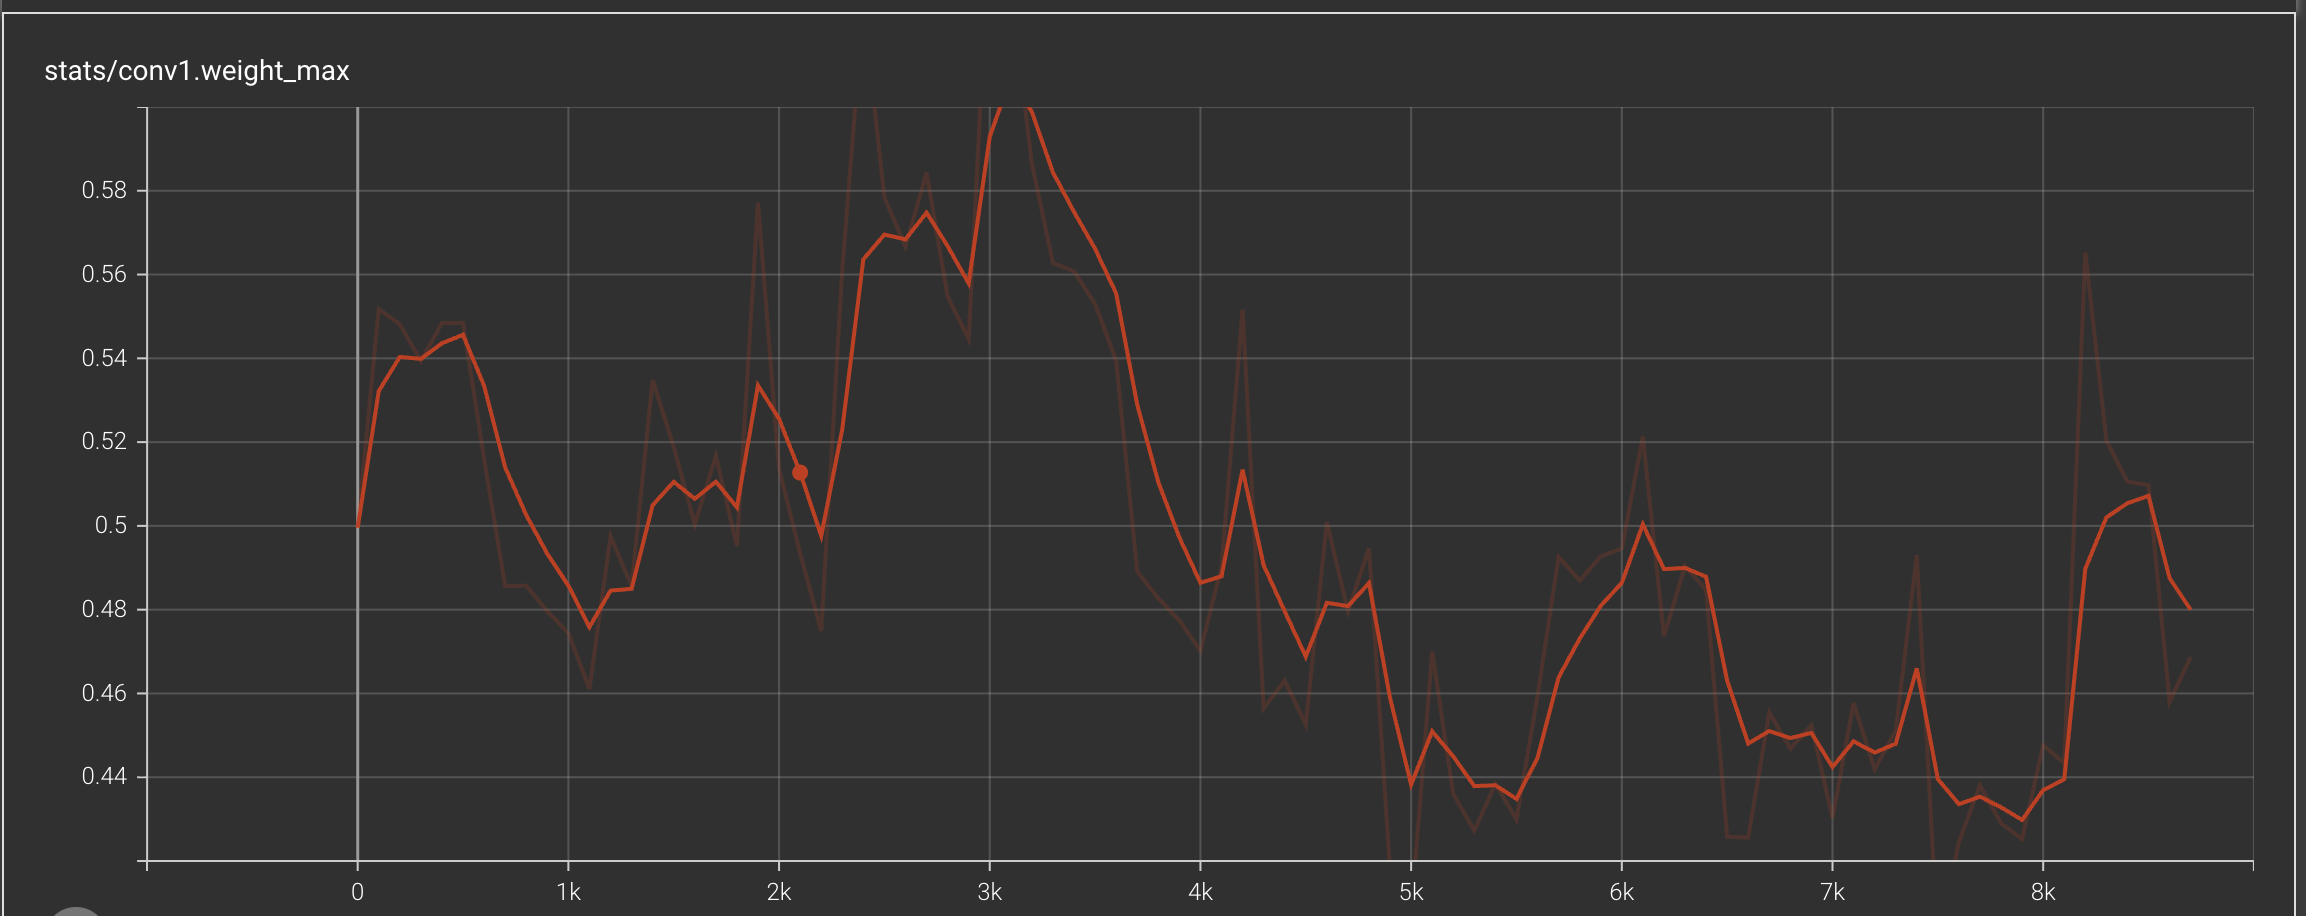
\includegraphics[width=.20\linewidth]{figs/tb_stats_params_conv1_weight_max.png}} &
\fbox{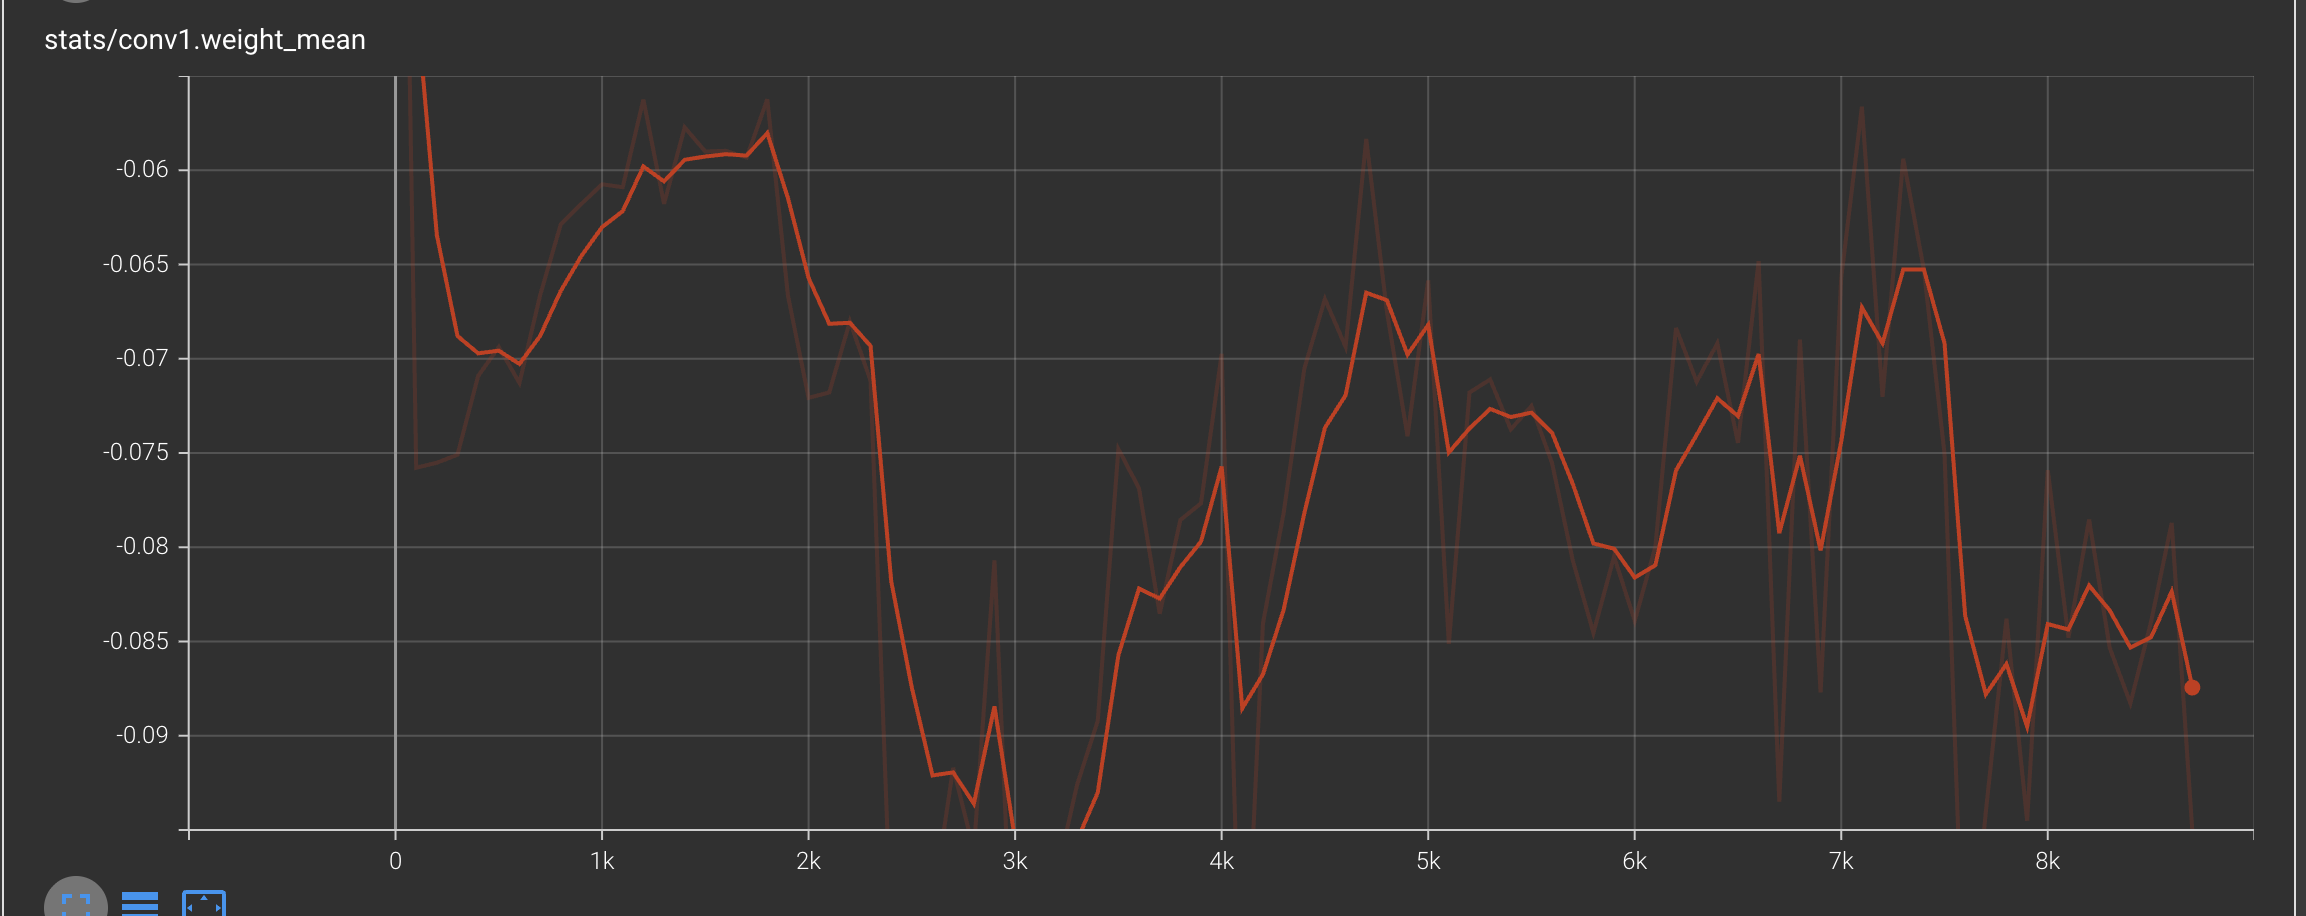
\includegraphics[width=.20\linewidth]{figs/tb_stats_params_conv1_weight_mean.png}} &
\fbox{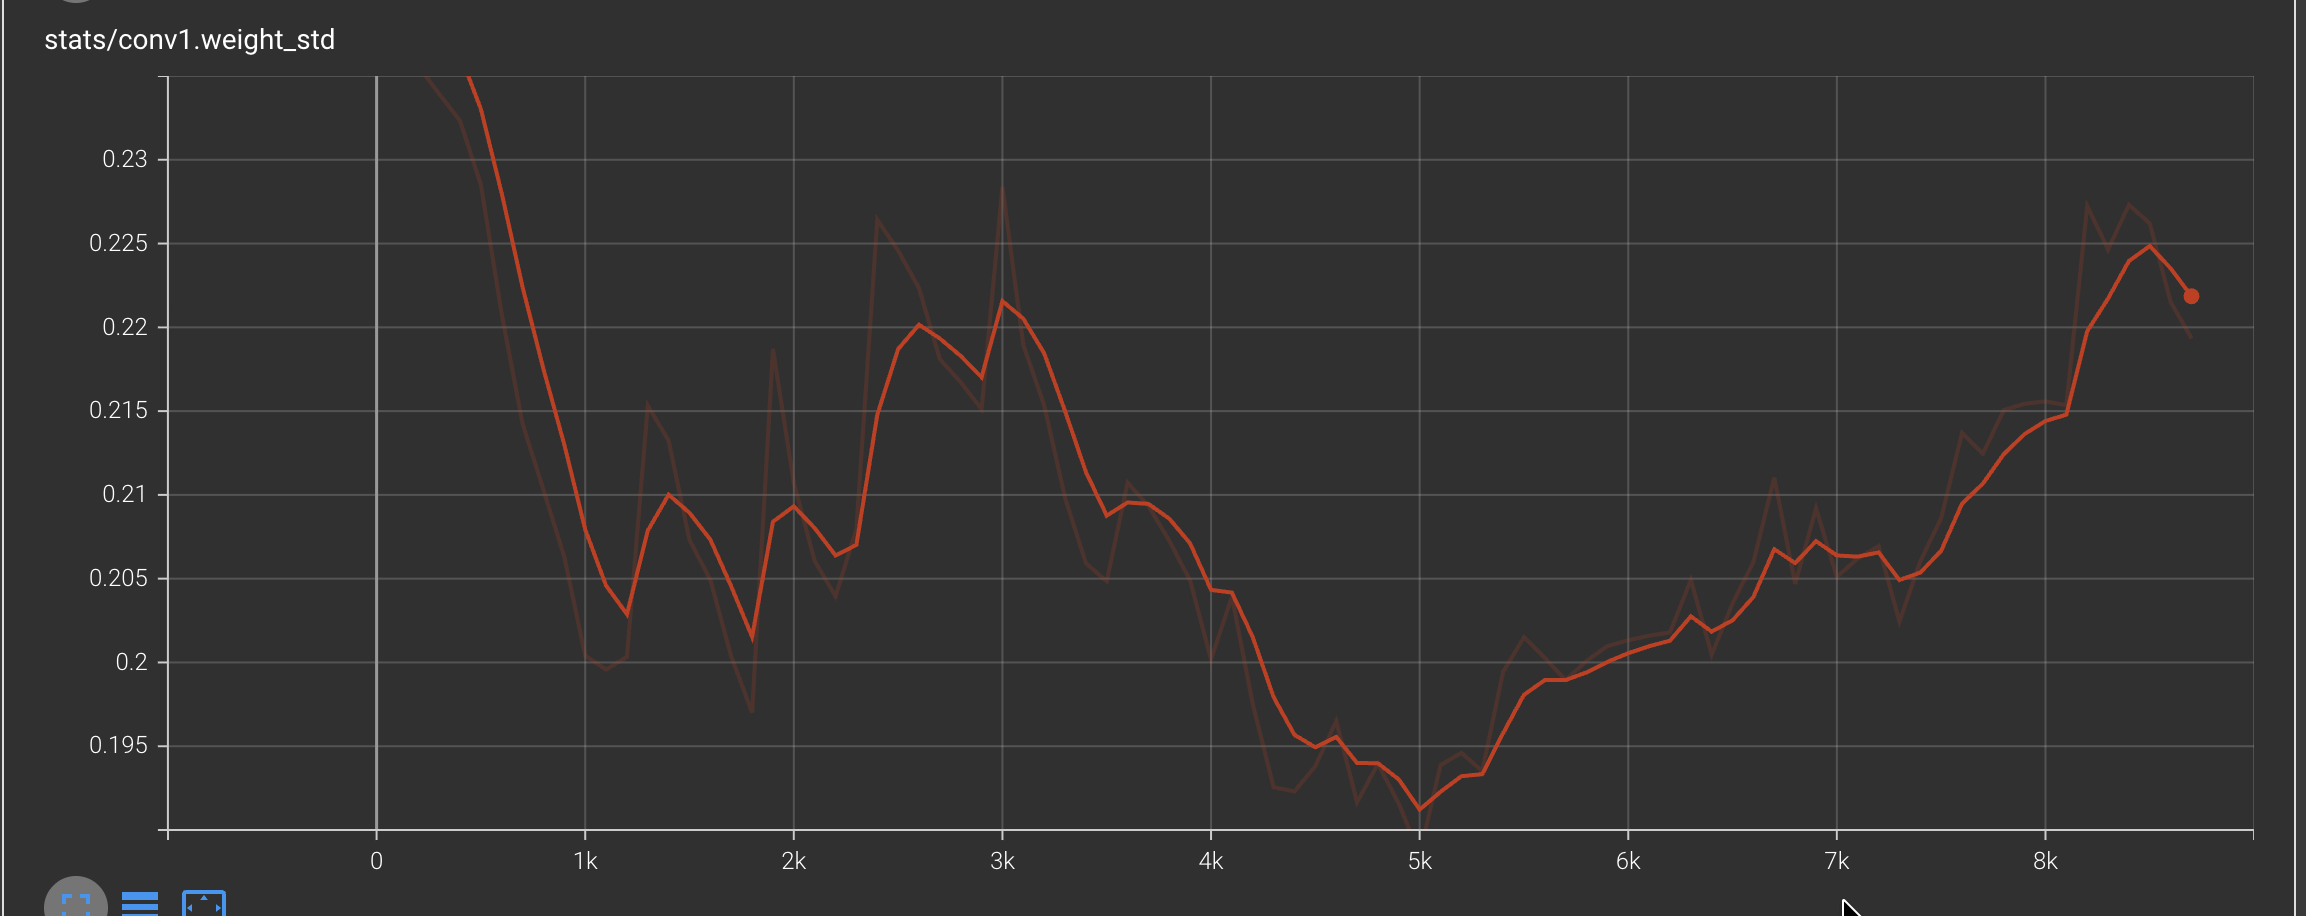
\includegraphics[width=.20\linewidth]{figs/tb_stats_params_conv1_weight_std.png}}\\
Weights min & Weights max & Weights mean & Weights std
\end{tabular}

\vspace{0.4em}

% Biases (conv1): min/max/mean/std
\begin{tabular}{cccc}
\fbox{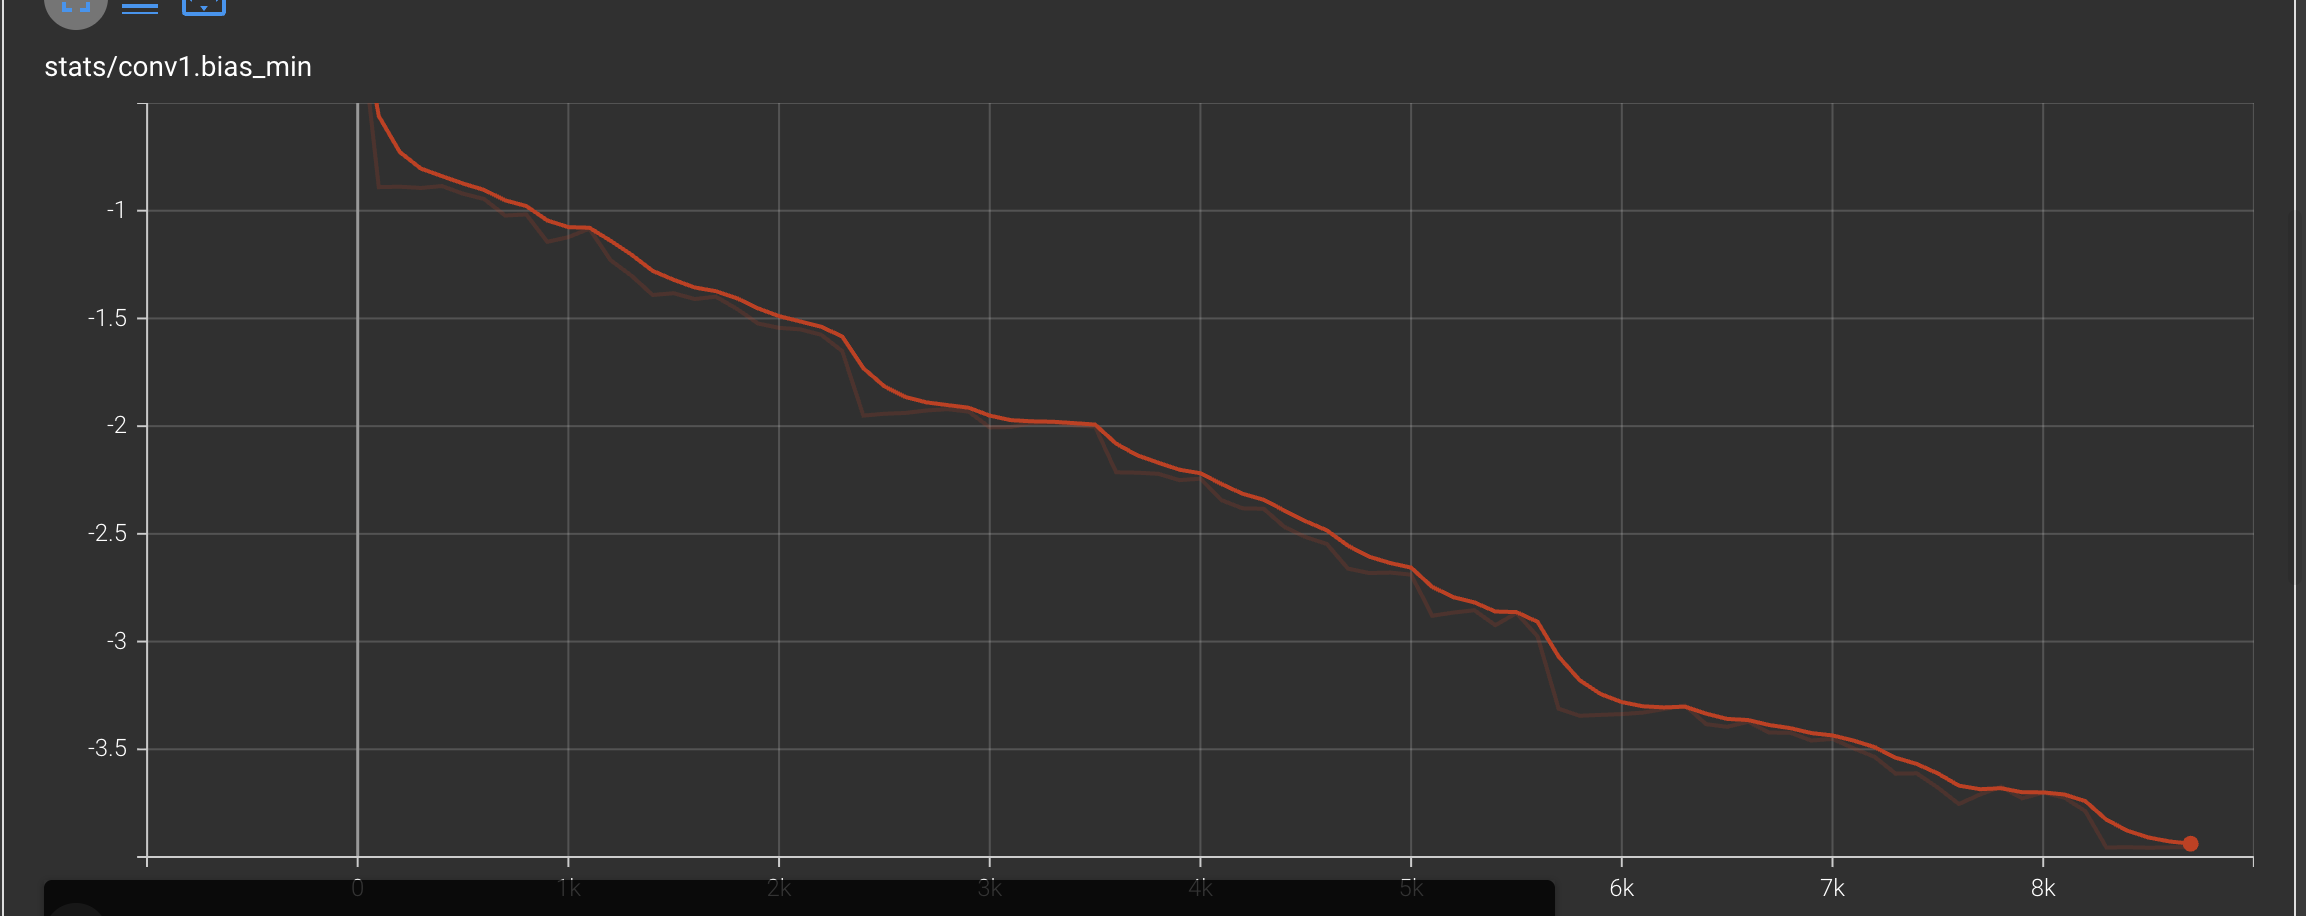
\includegraphics[width=.20\linewidth]{figs/tb_stats_params_conv1_bias_min.png}} &
\fbox{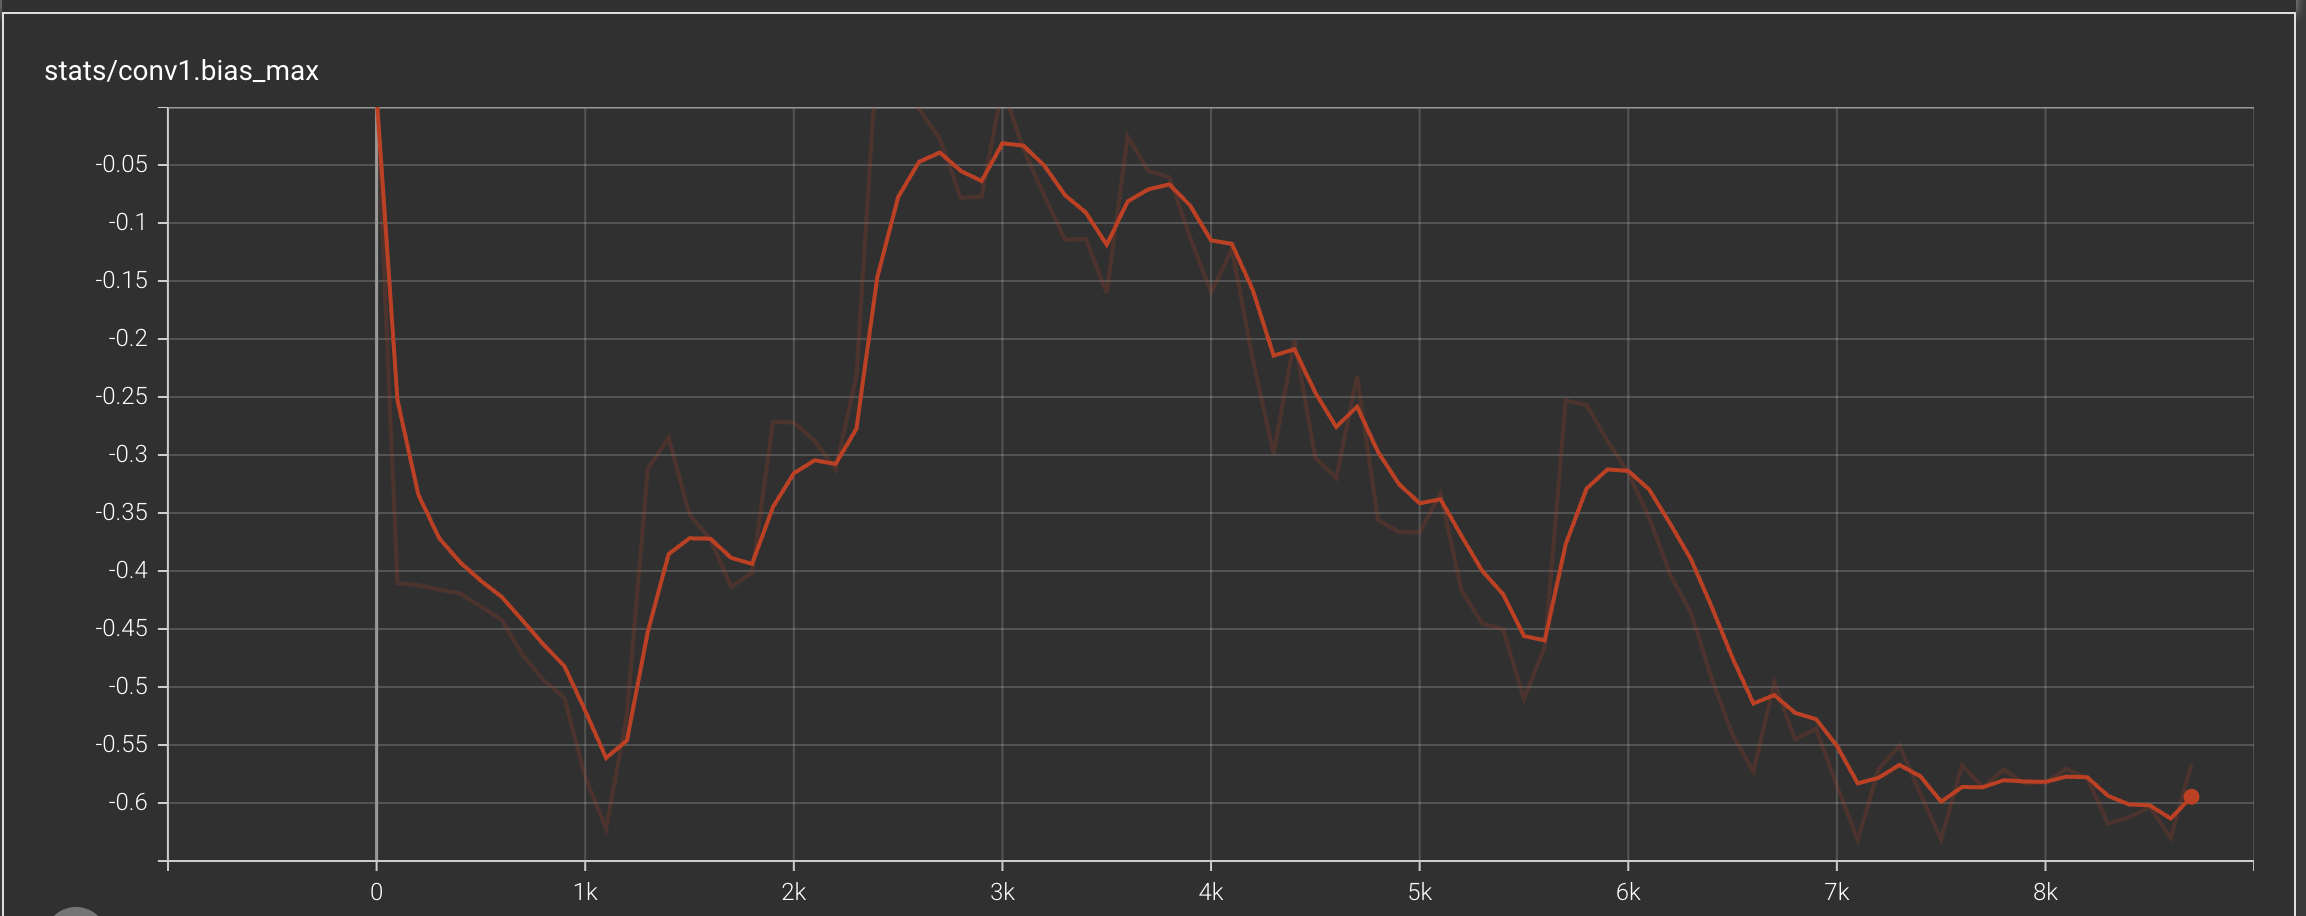
\includegraphics[width=.20\linewidth]{figs/tb_stats_params_conv1_bias_max.png}} &
\fbox{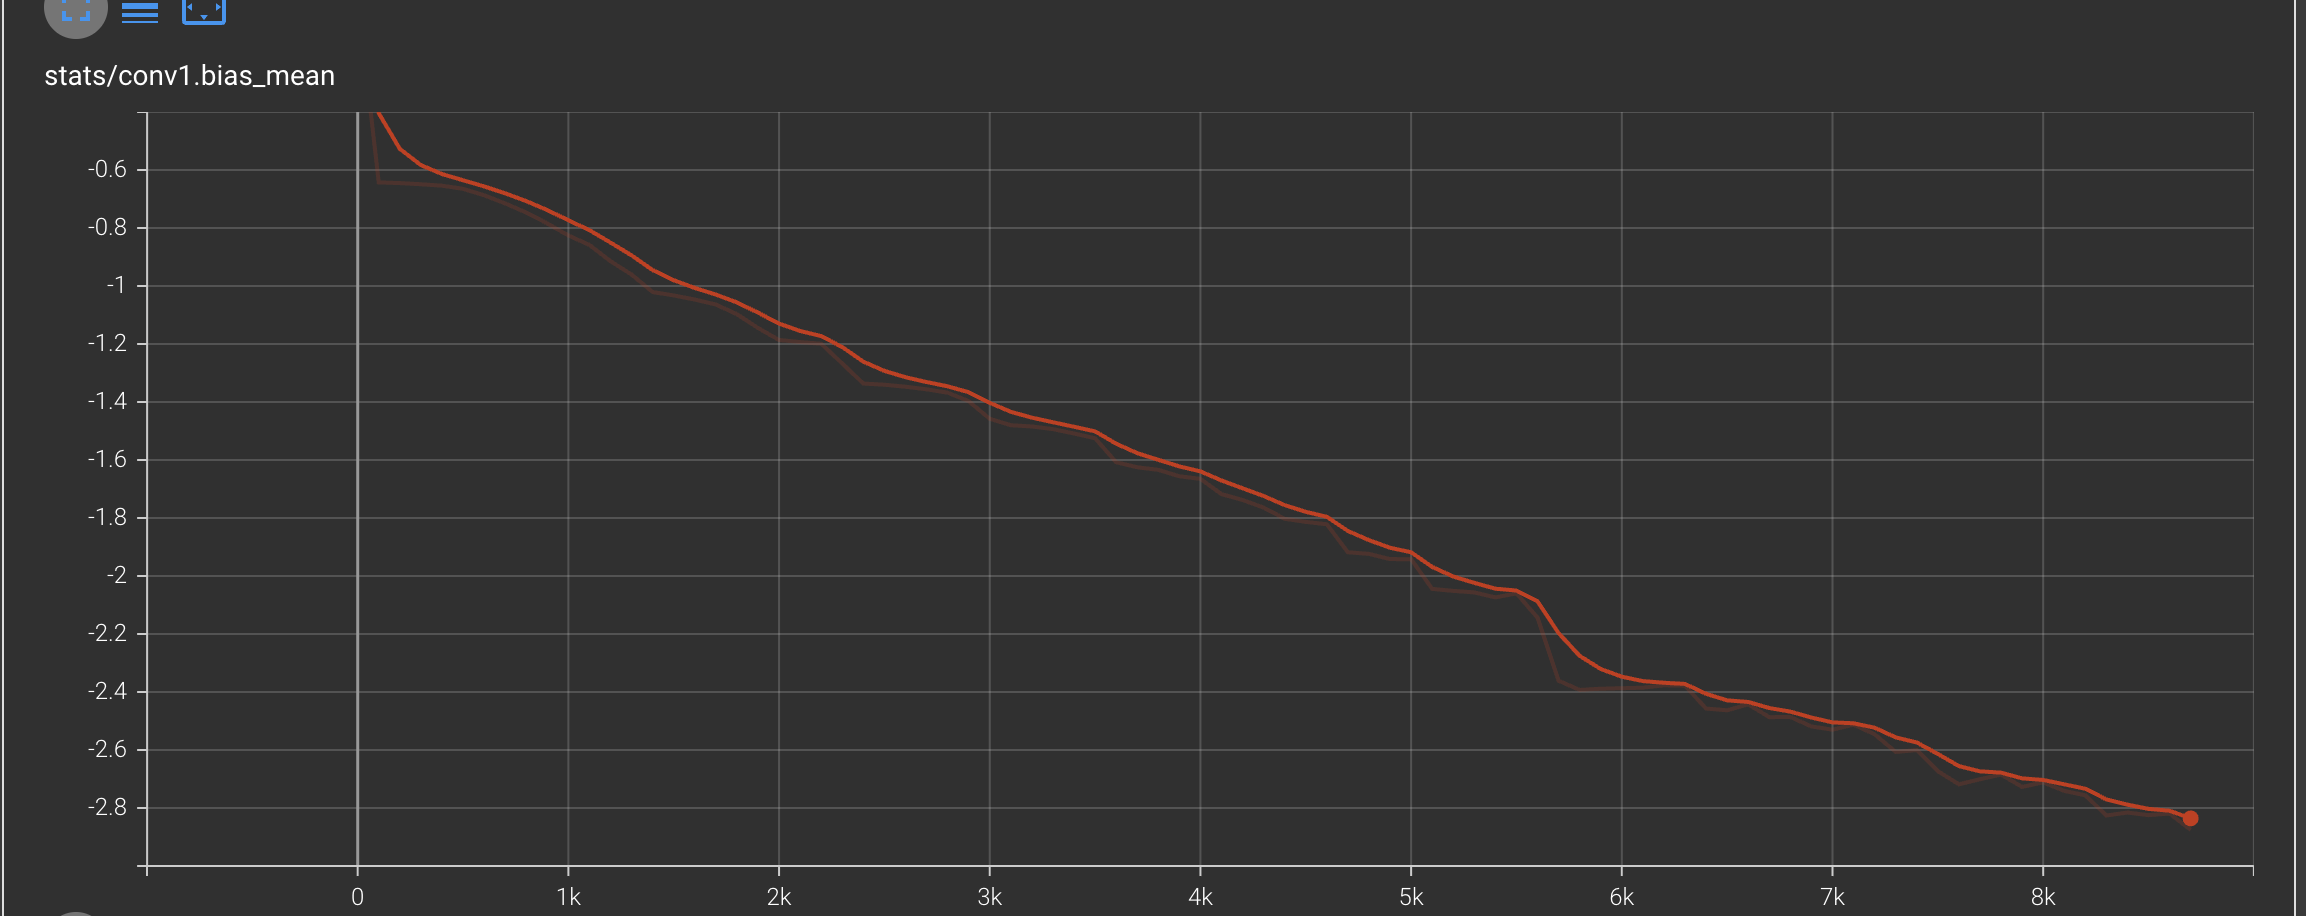
\includegraphics[width=.20\linewidth]{figs/tb_stats_params_conv1_bias_mean.png}} &
\fbox{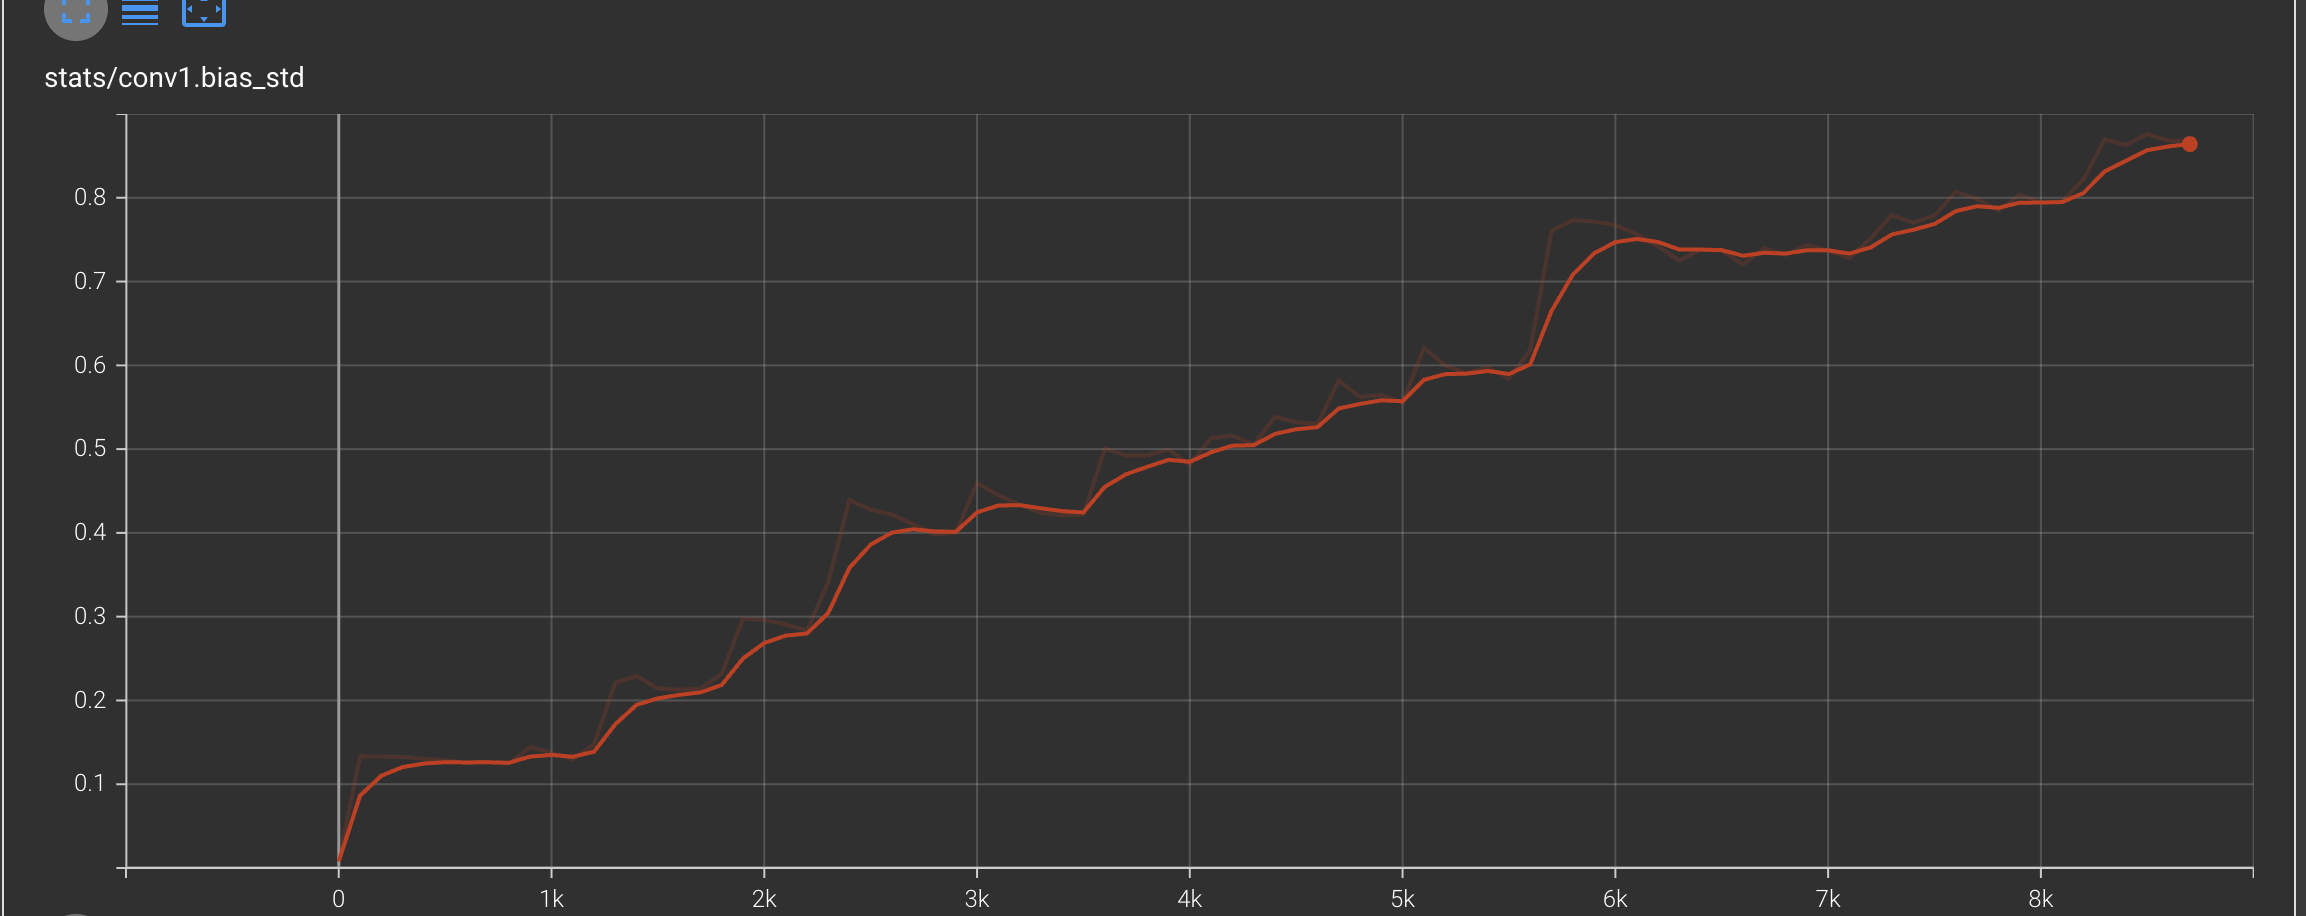
\includegraphics[width=.20\linewidth]{figs/tb_stats_params_conv1_bias_std.png}}\\
Biases min & Biases max & Biases mean & Biases std
\end{tabular}

\vspace{0.4em}

% Net inputs z (conv1): min/max/mean/std
\begin{tabular}{cccc}
\fbox{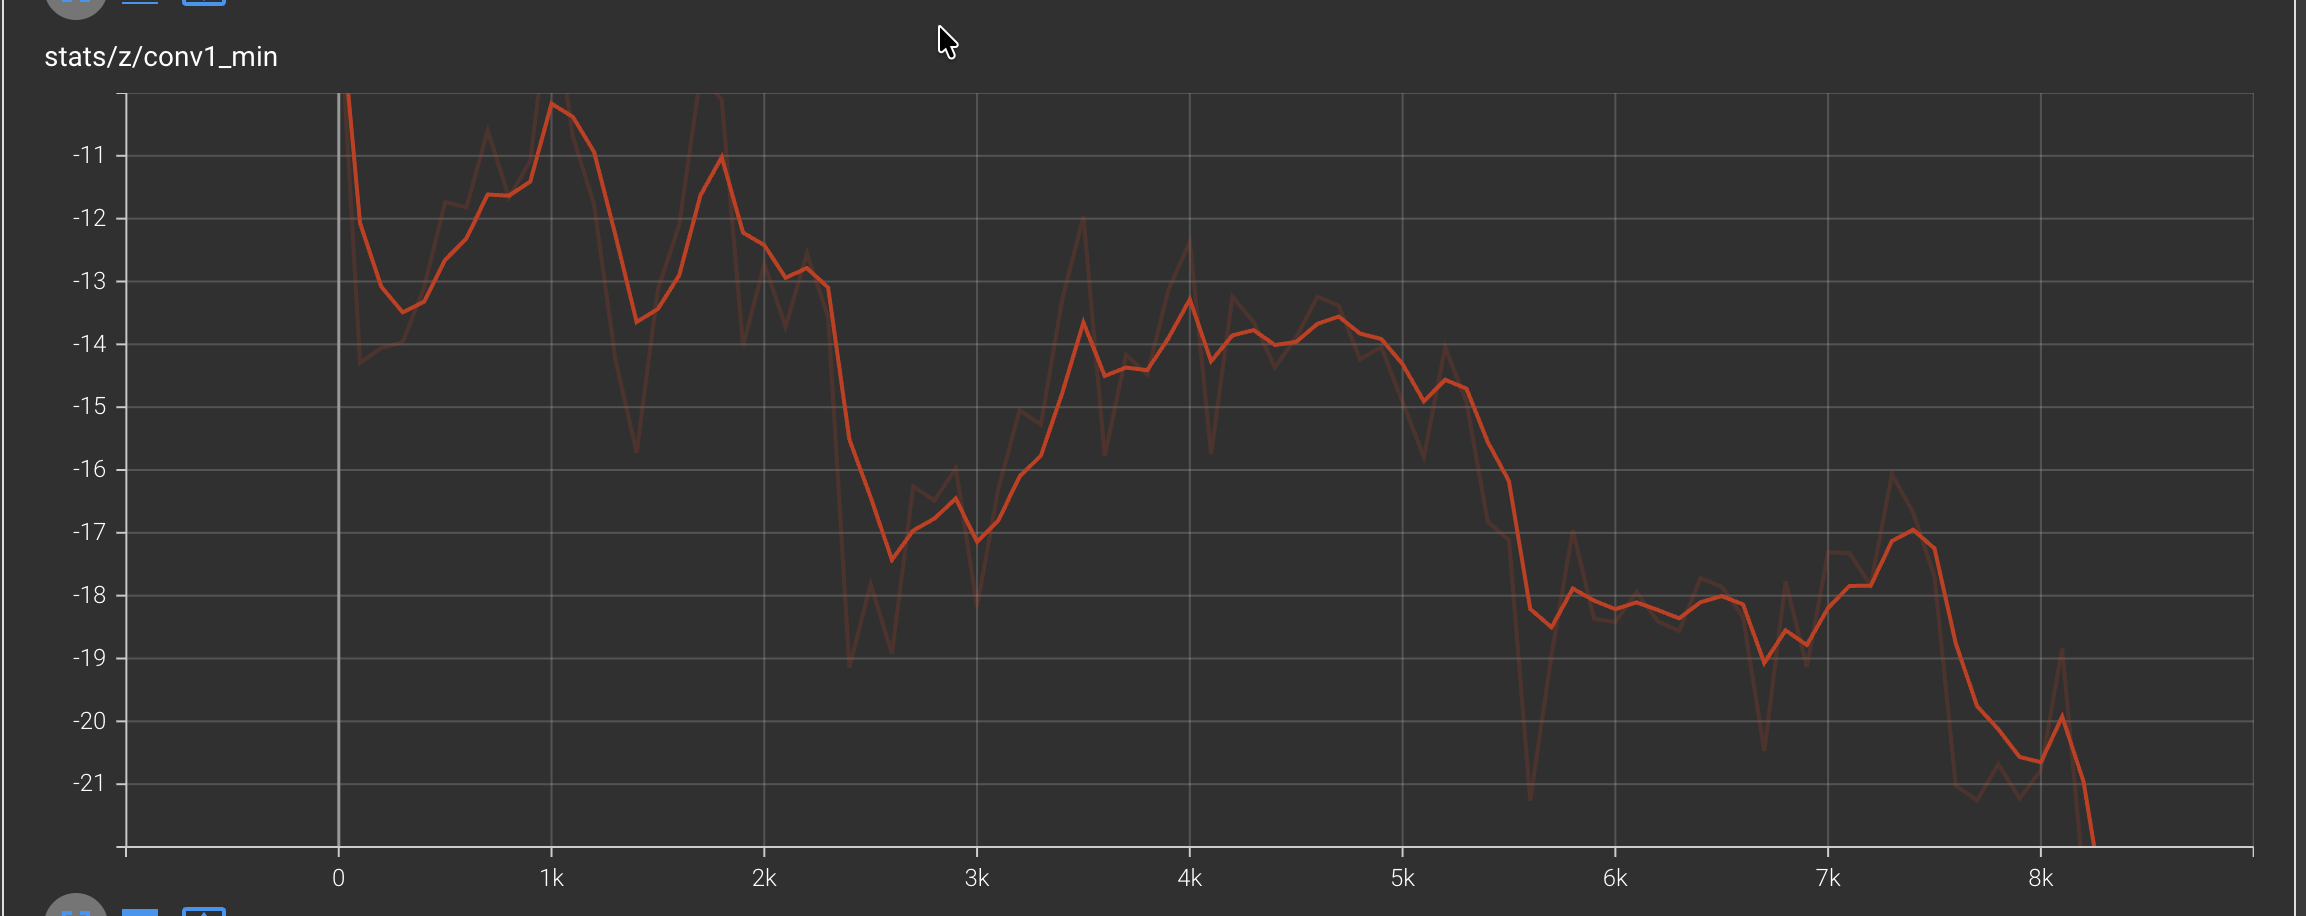
\includegraphics[width=.20\linewidth]{figs/tb_stats_z_conv1_min.png}} &
\fbox{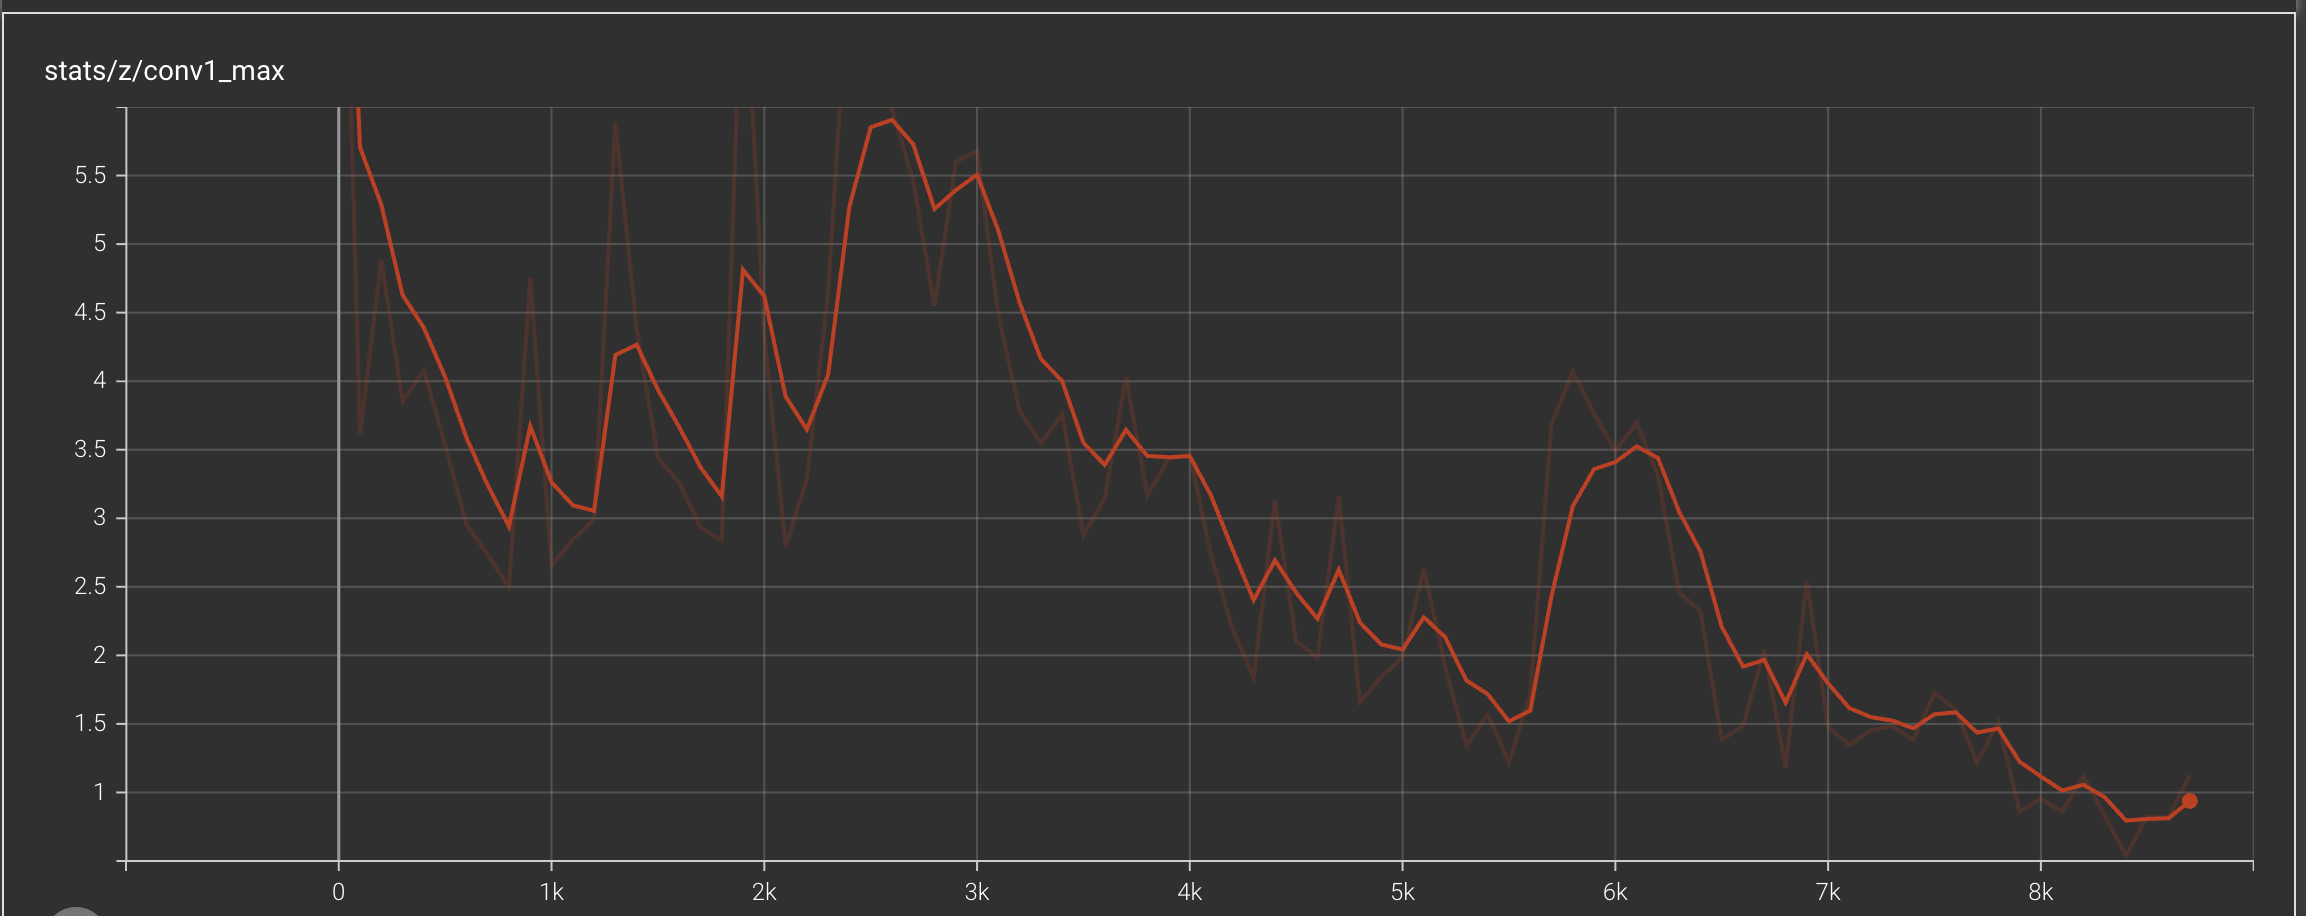
\includegraphics[width=.20\linewidth]{figs/tb_stats_z_conv1_max.png}} &
\fbox{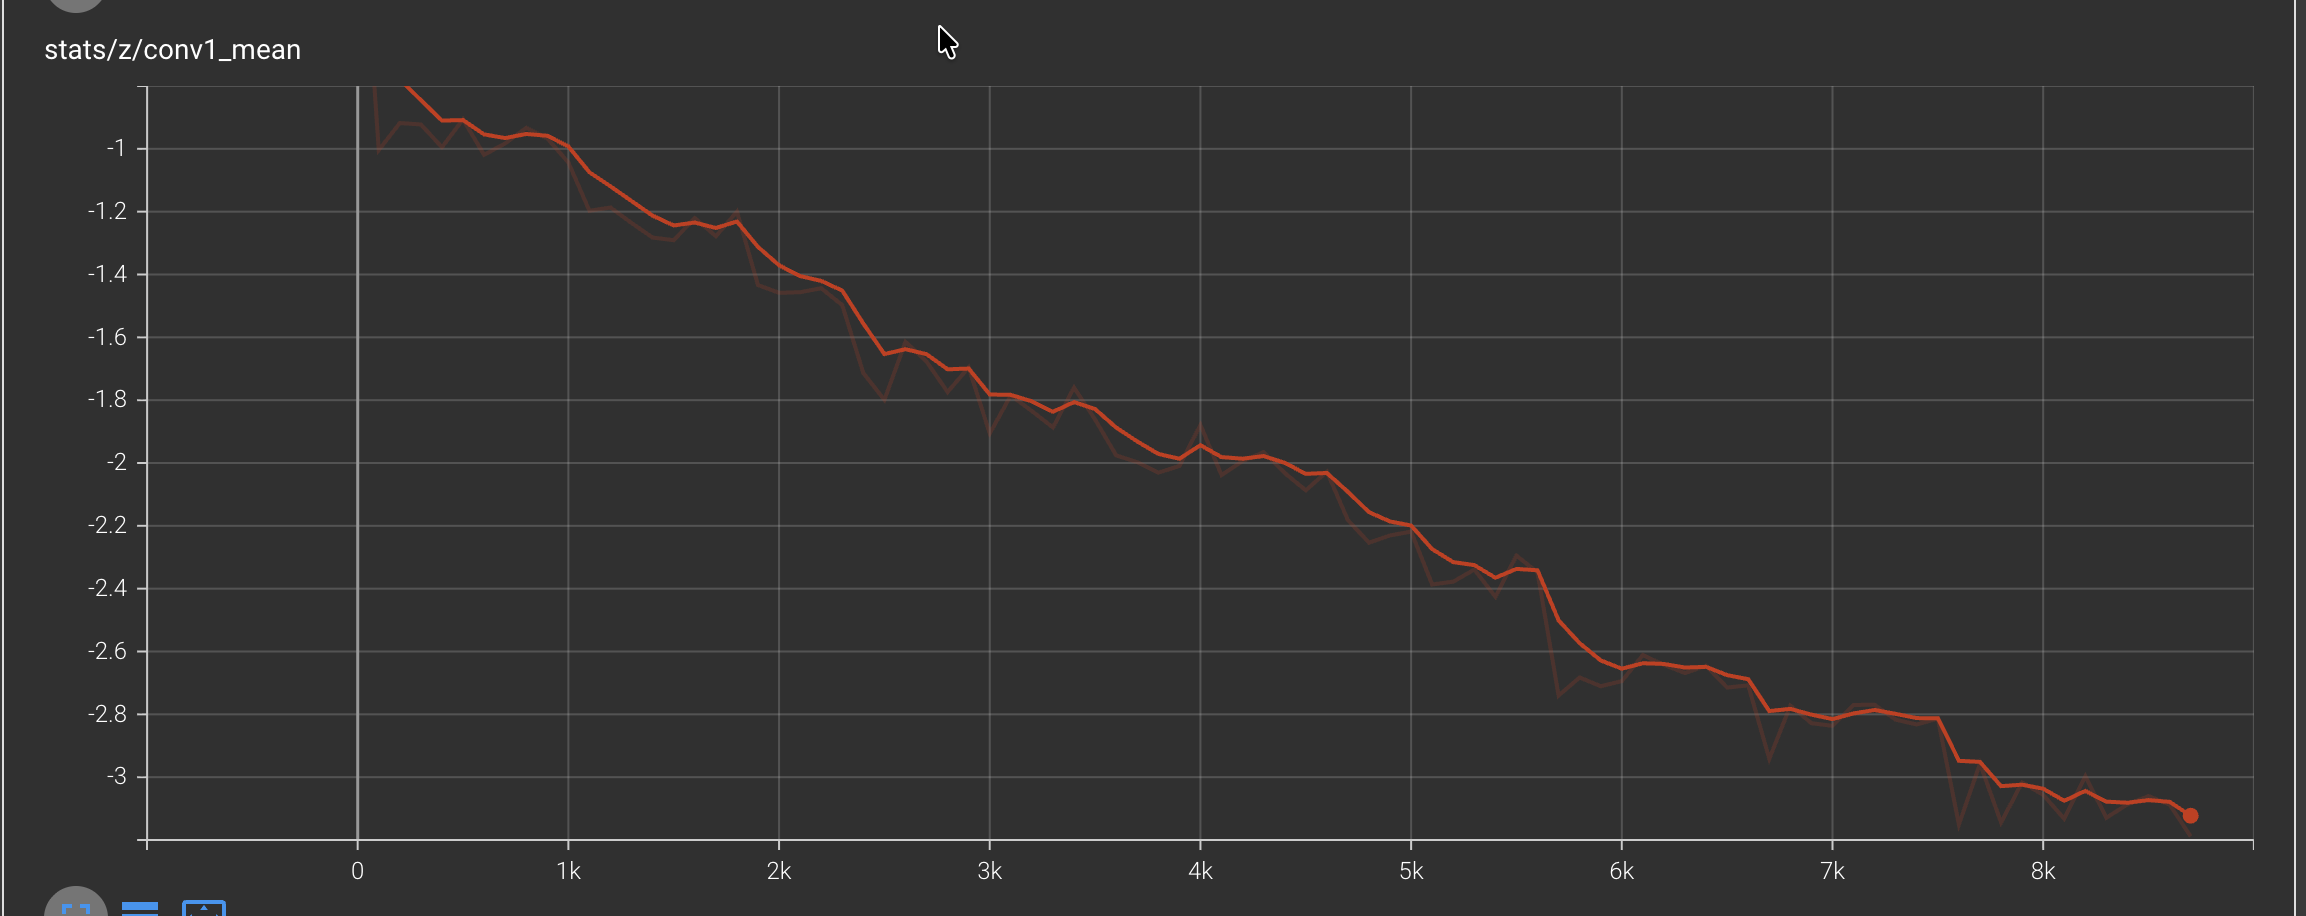
\includegraphics[width=.20\linewidth]{figs/tb_stats_z_conv1_mean.png}} &
\fbox{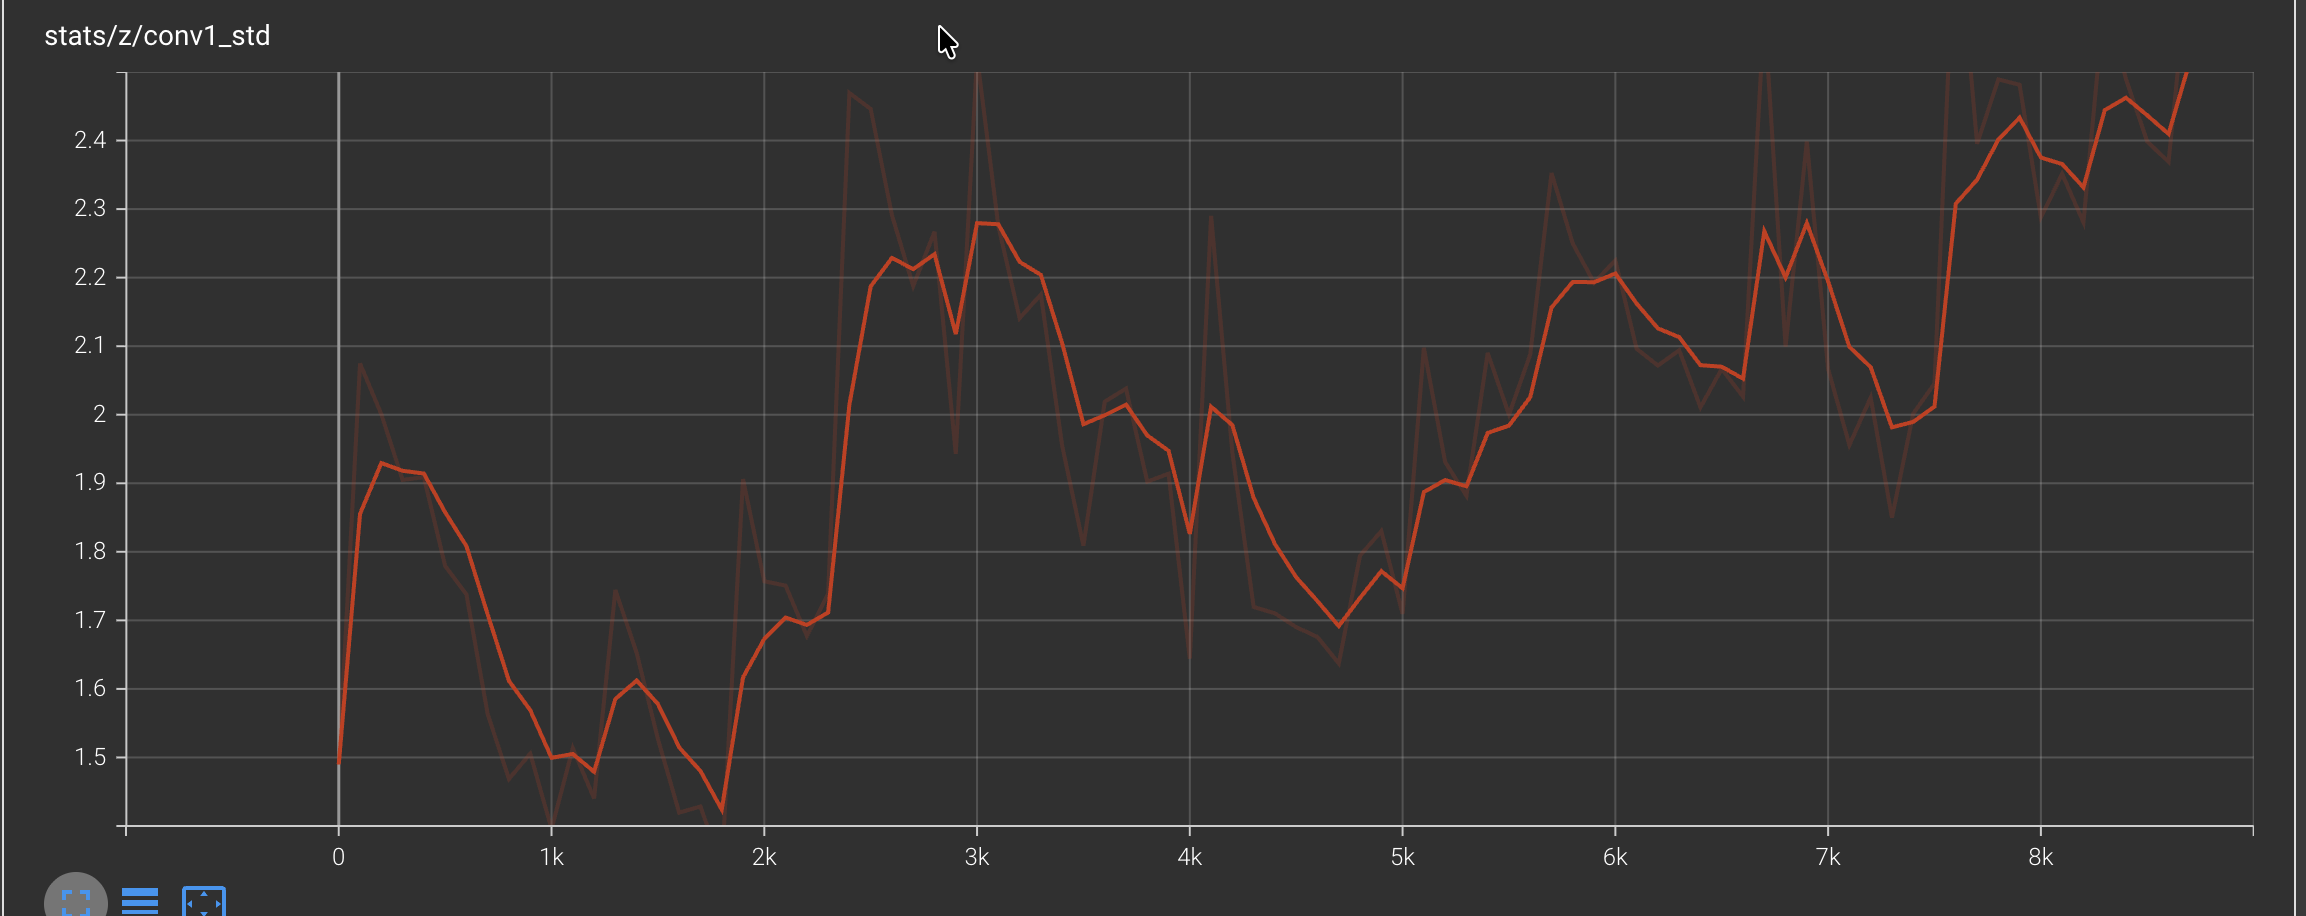
\includegraphics[width=.20\linewidth]{figs/tb_stats_z_conv1_std.png}}\\
Net input $z$ min & Net input $z$ max & Net input $z$ mean & Net input $z$ std
\end{tabular}

\vspace{0.4em}

% Post-ReLU (layer 1): min/max/mean/std
\begin{tabular}{cccc}
\fbox{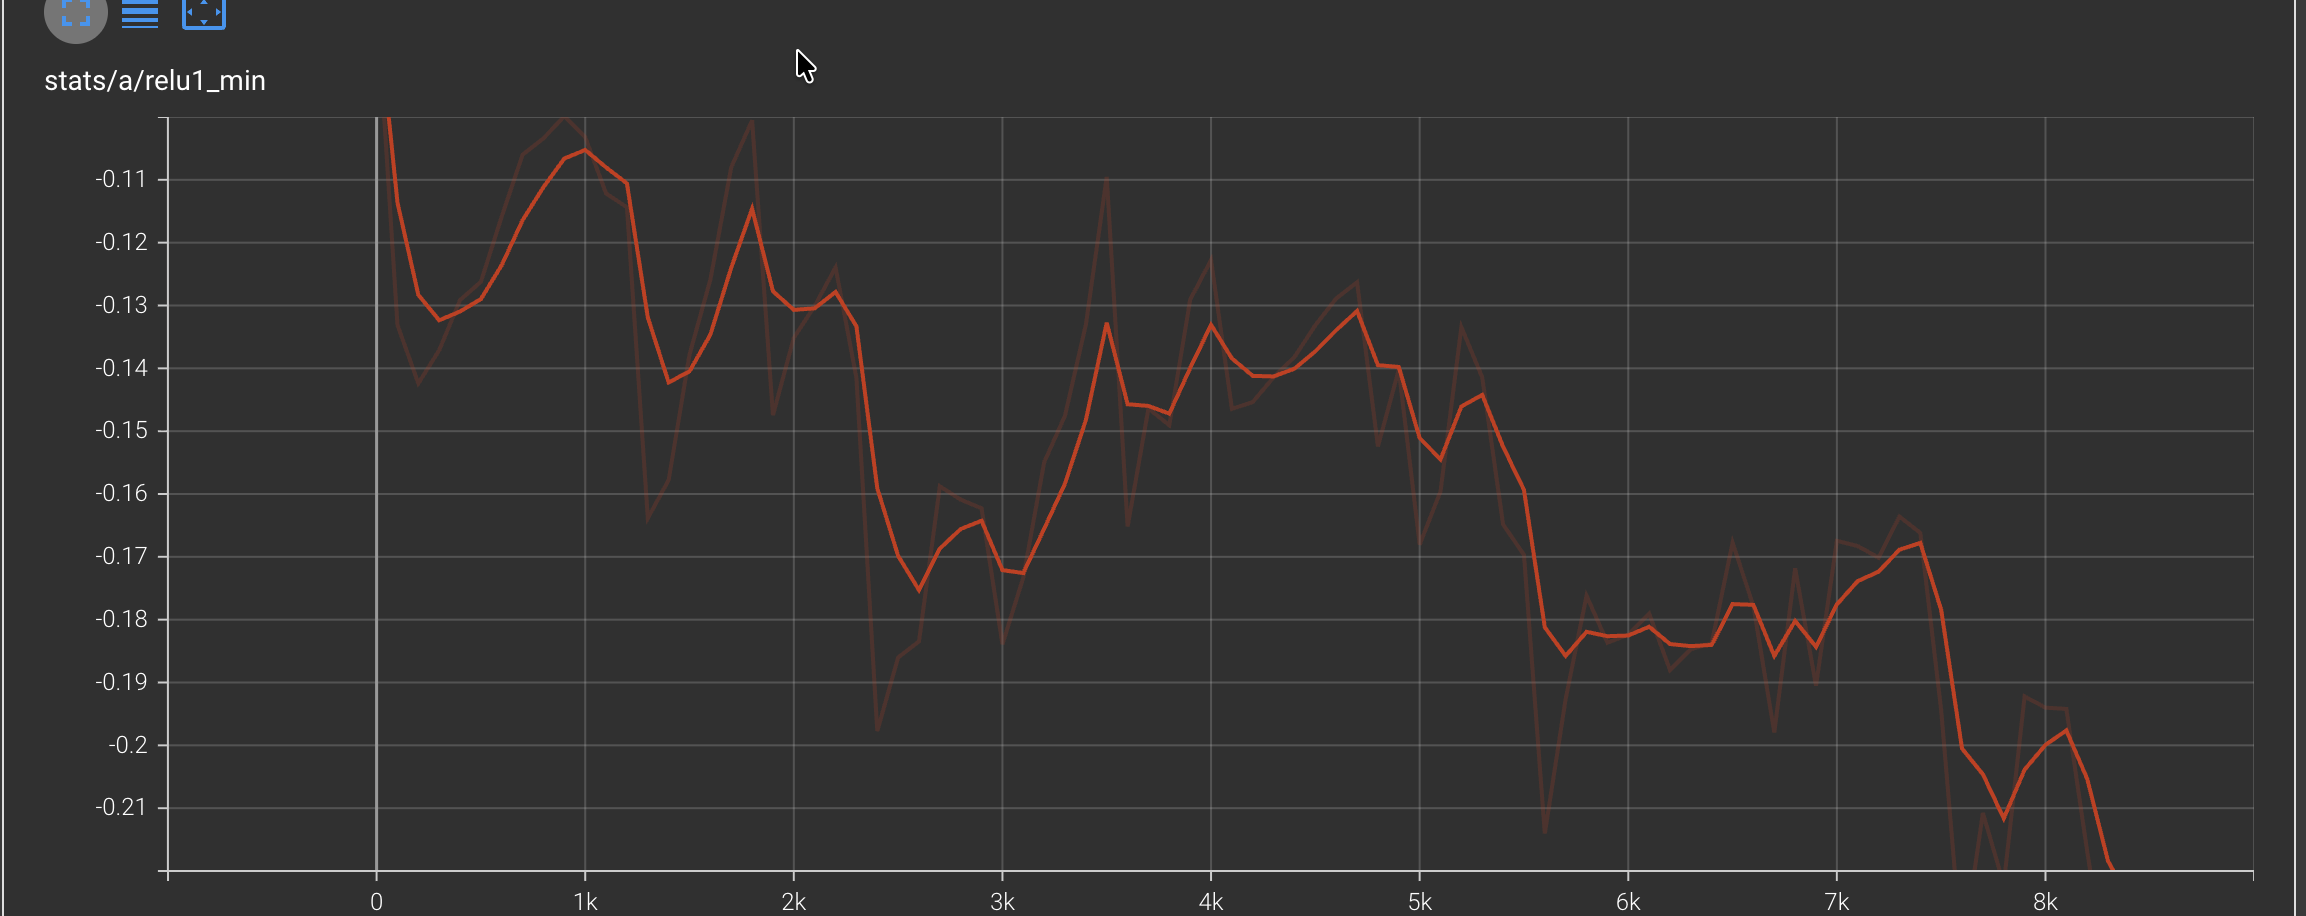
\includegraphics[width=.20\linewidth]{figs/tb_stats_a_relu1_min.png}} &
\fbox{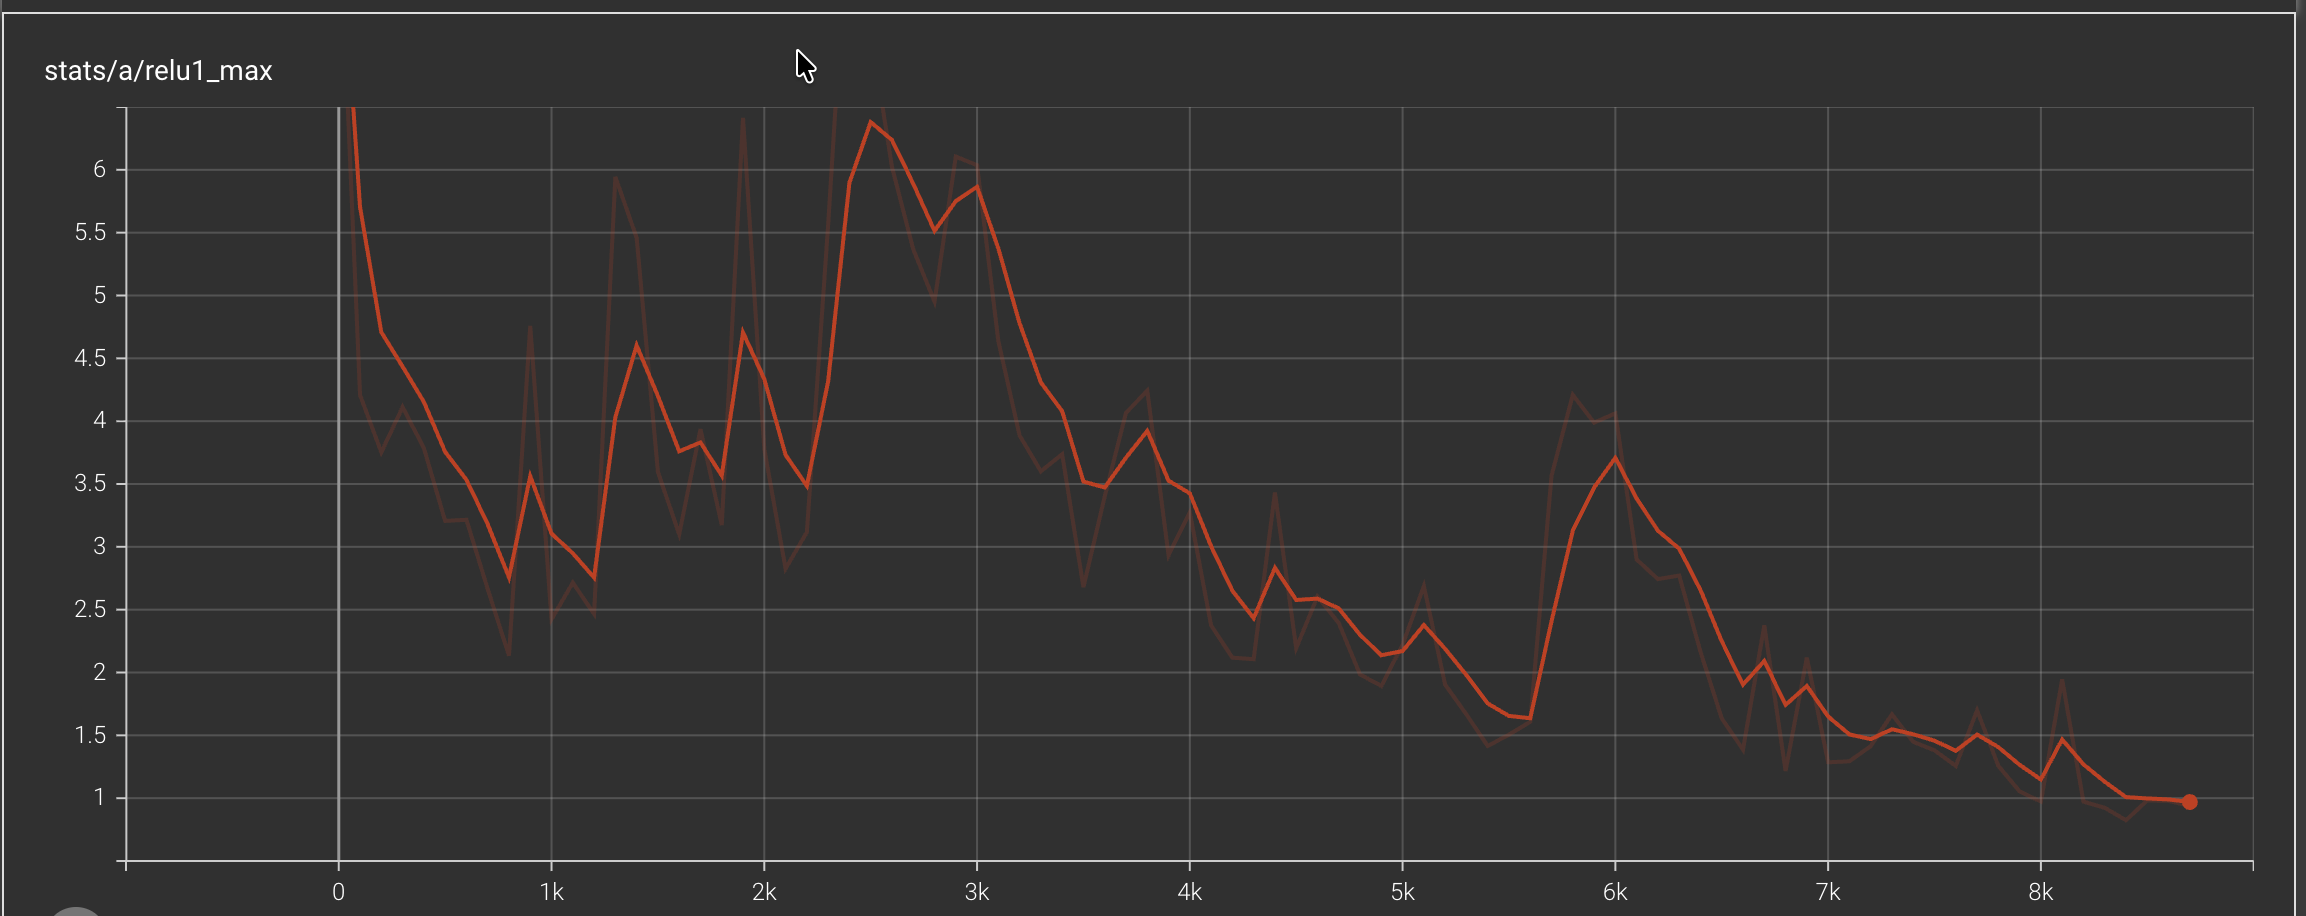
\includegraphics[width=.20\linewidth]{figs/tb_stats_a_relu1_max.png}} &
\fbox{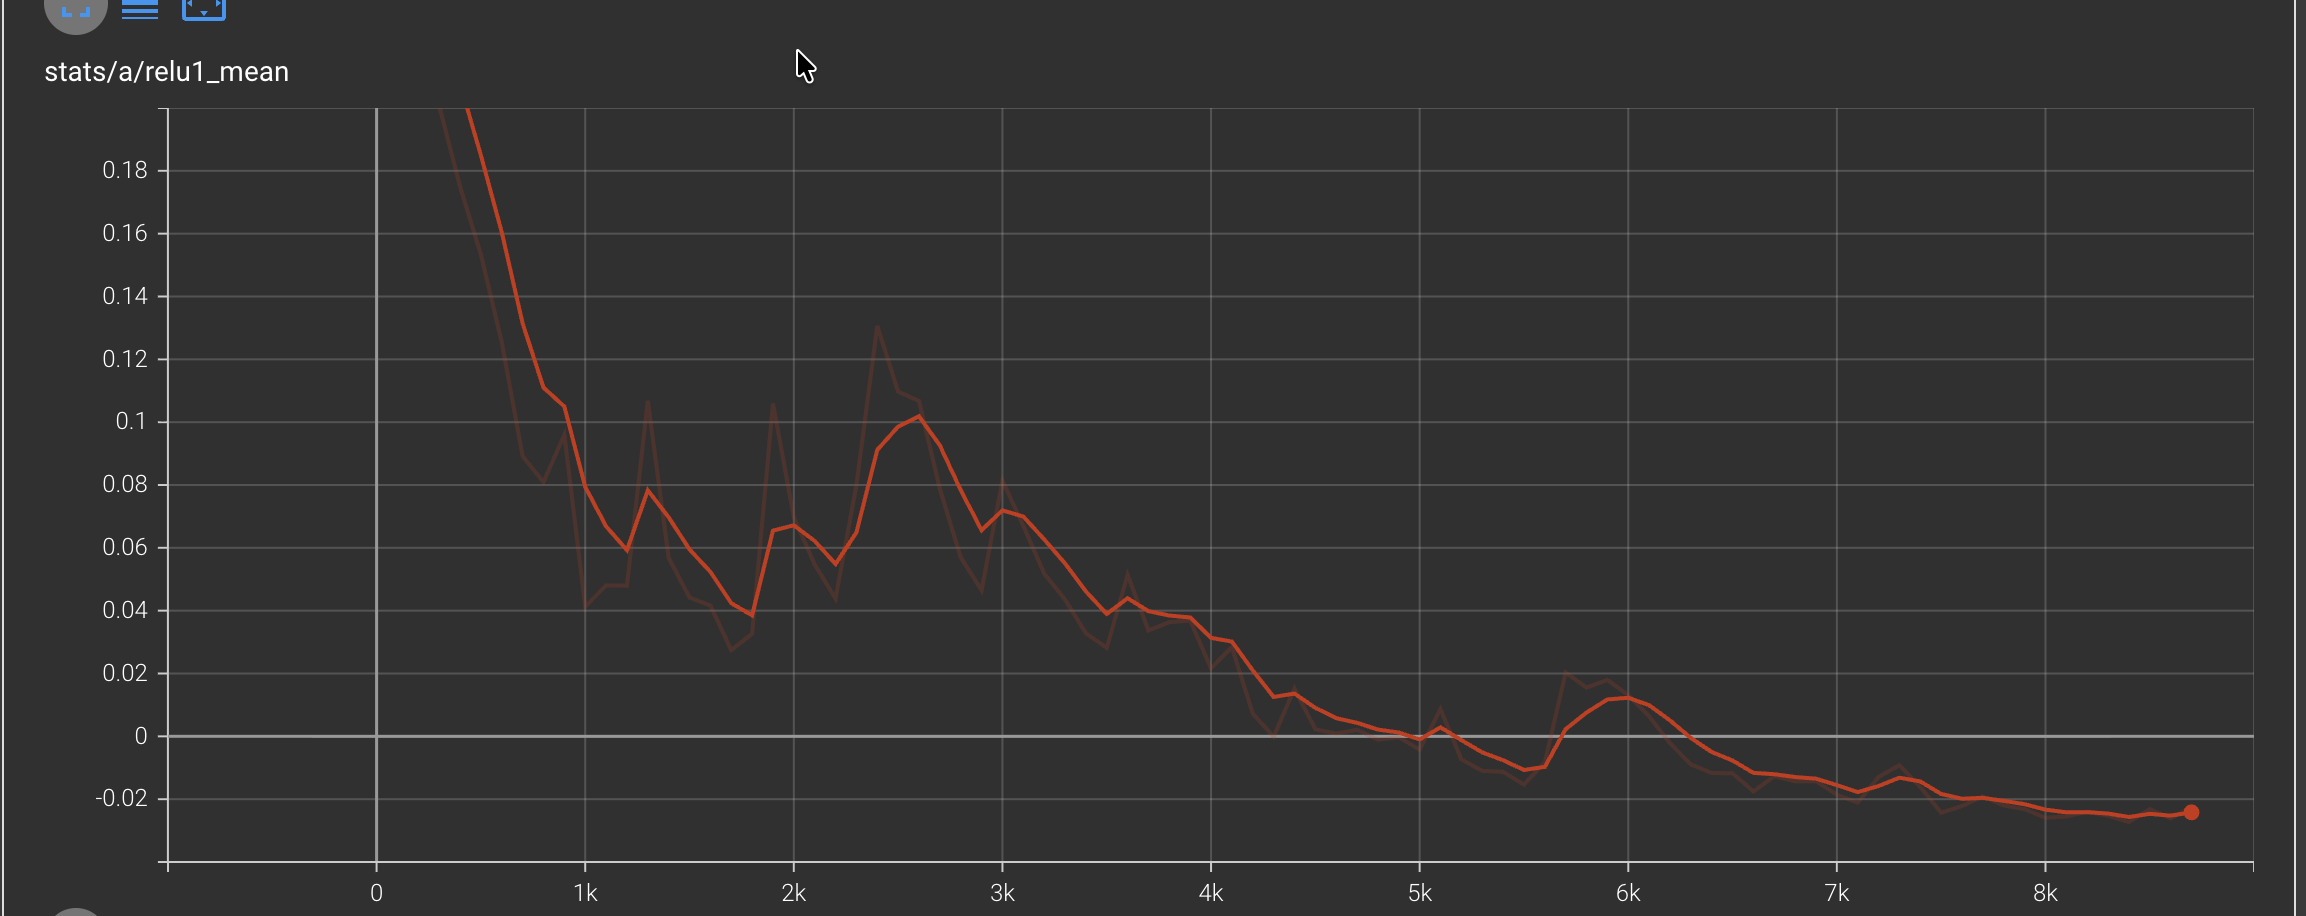
\includegraphics[width=.20\linewidth]{figs/tb_stats_a_relu1_mean.png}} &
\fbox{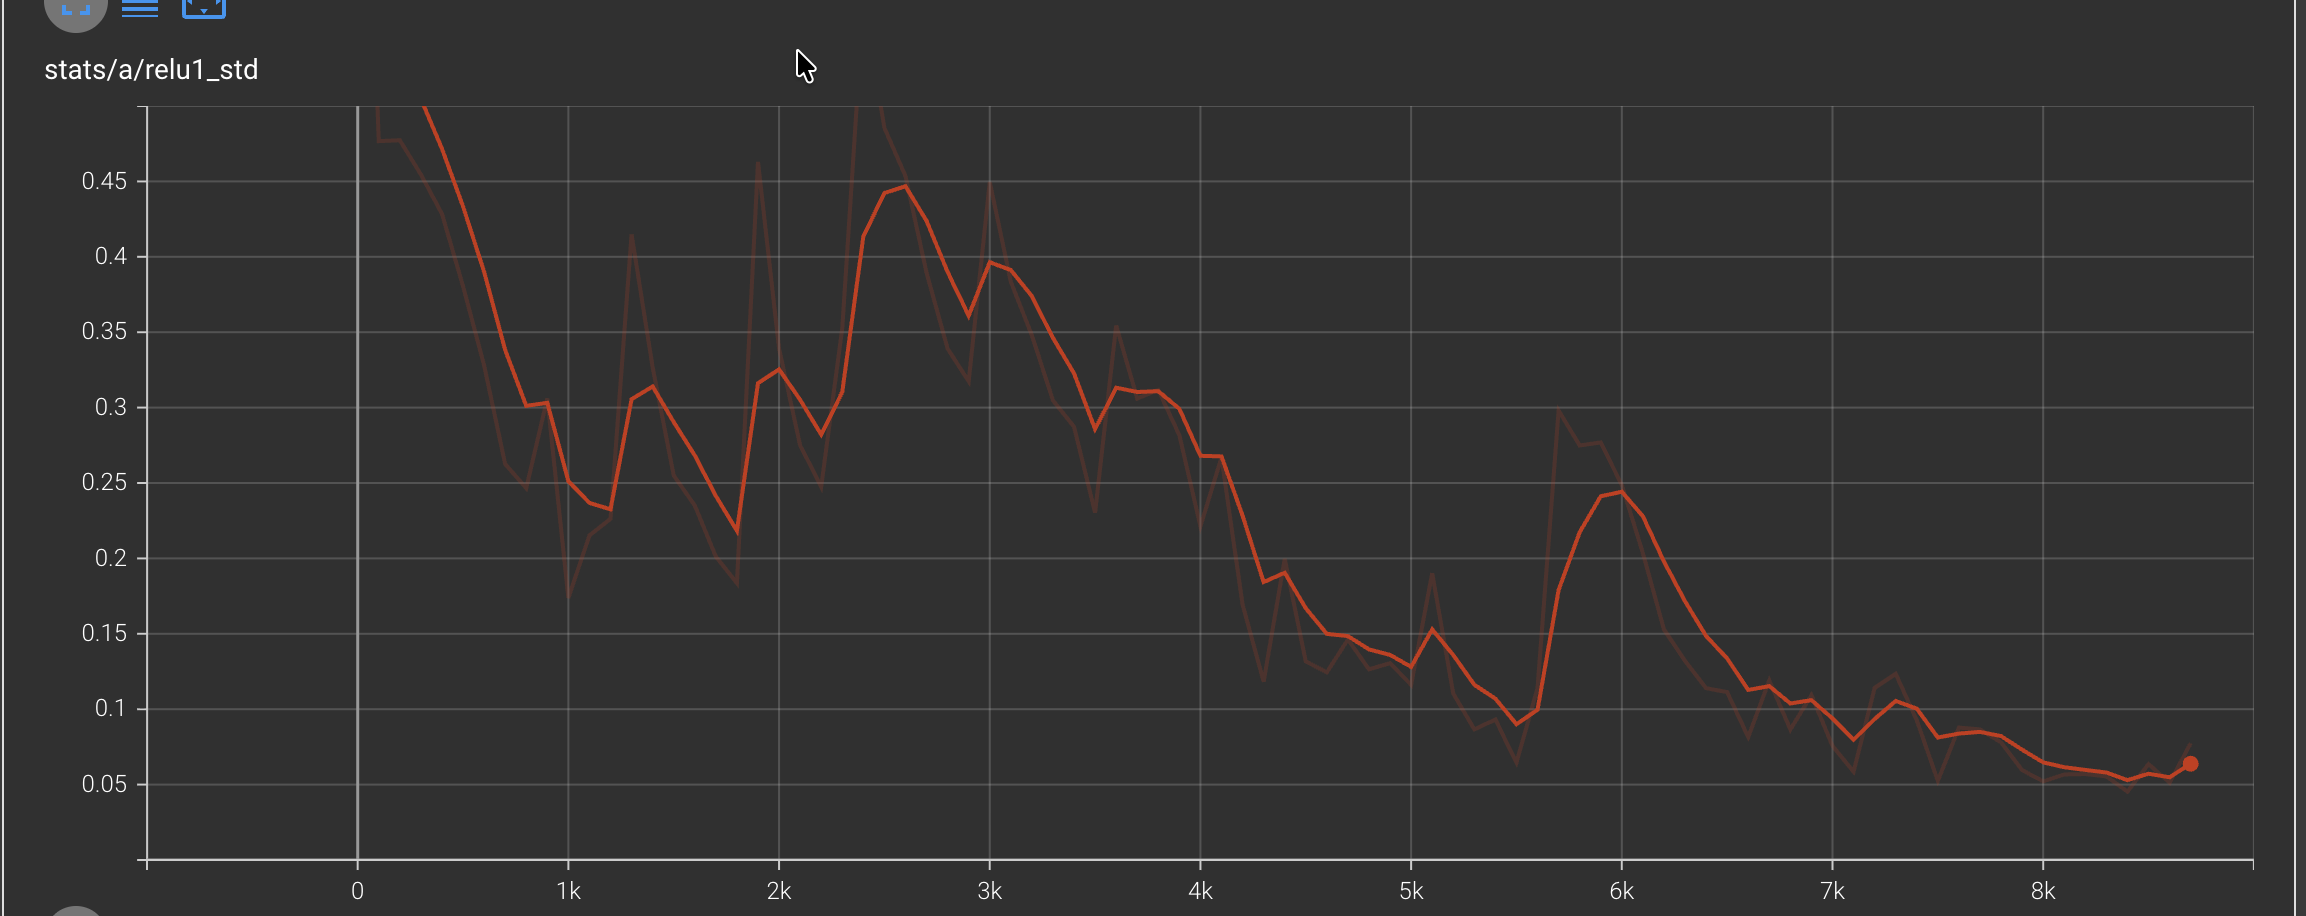
\includegraphics[width=.20\linewidth]{figs/tb_stats_a_relu1_std.png}}\\
Post-ReLU min & Post-ReLU max & Post-ReLU mean & Post-ReLU std
\end{tabular}

\vspace{0.4em}

% Post-MaxPool (pool1): min/max/mean/std
\begin{tabular}{cccc}
\fbox{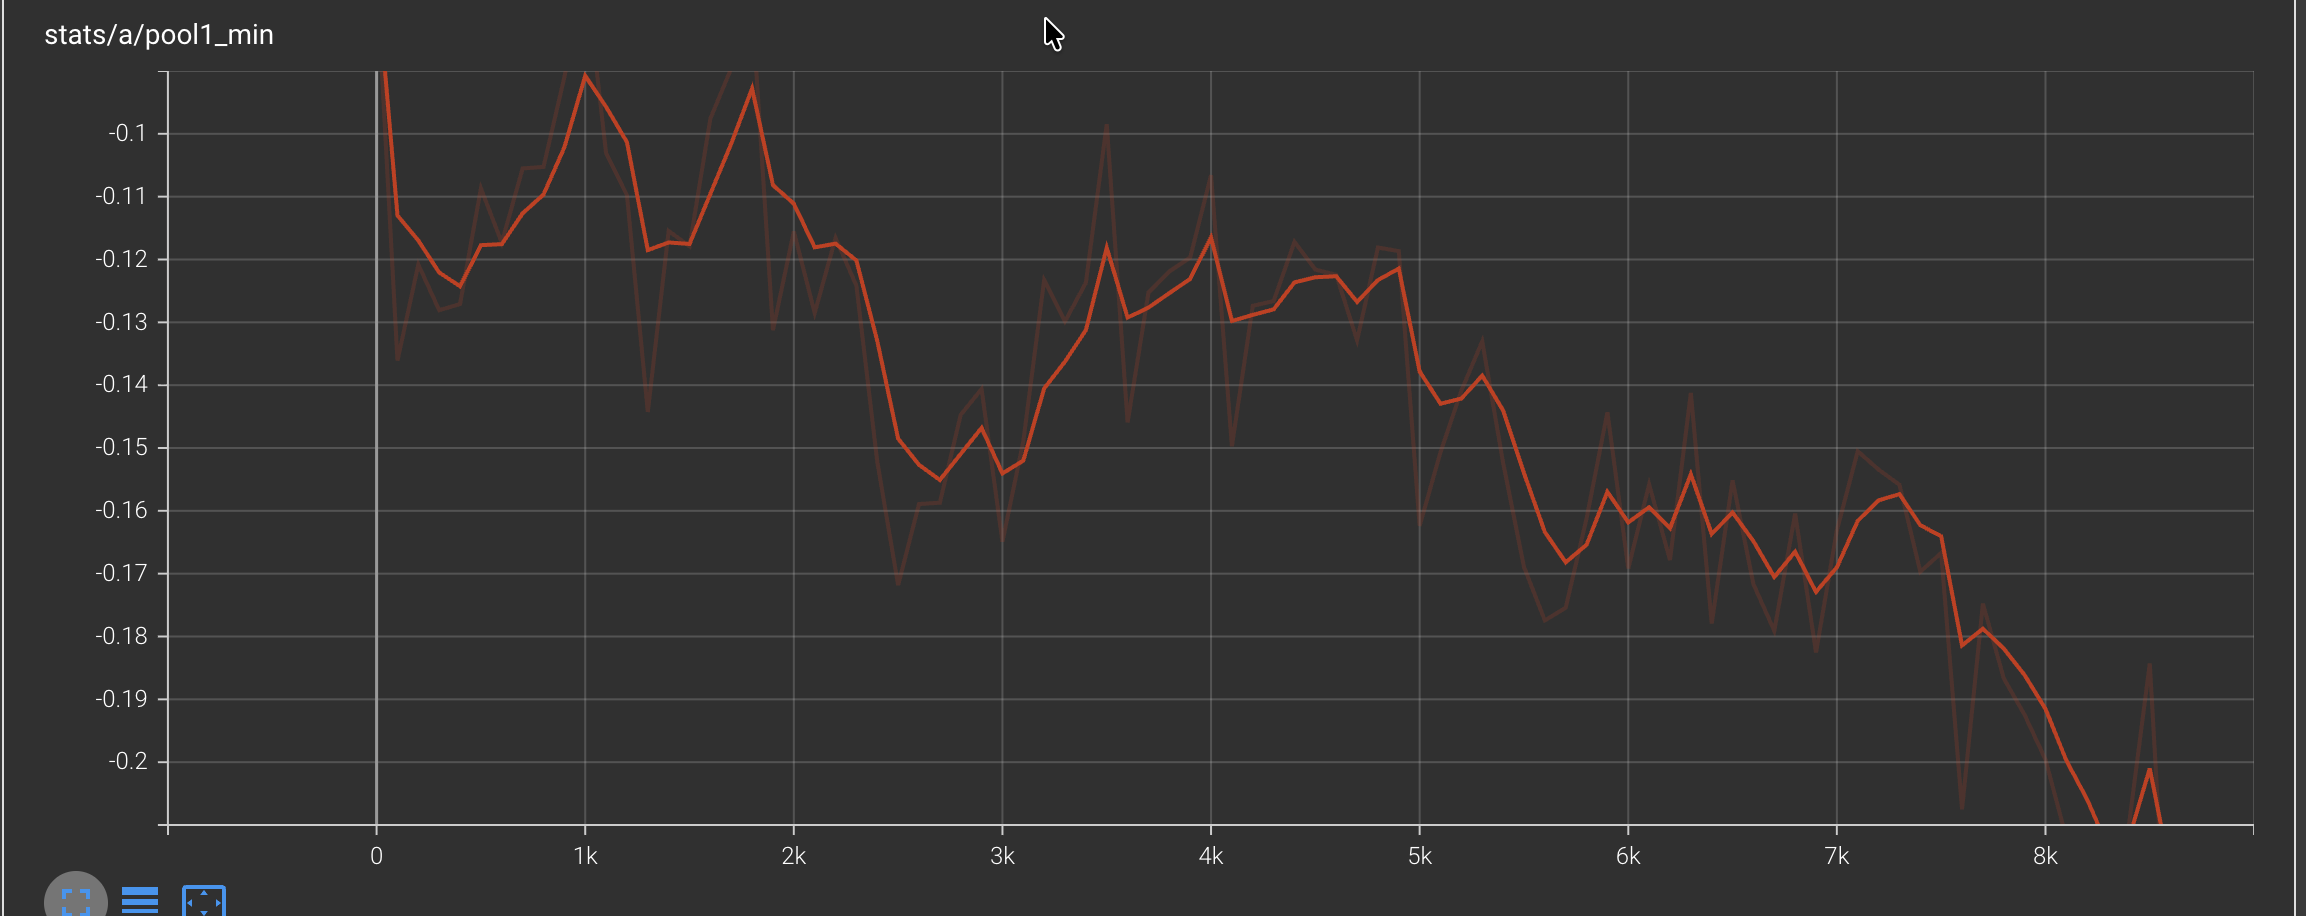
\includegraphics[width=.20\linewidth]{figs/tb_stats_a_pool1_min.png}} &
\fbox{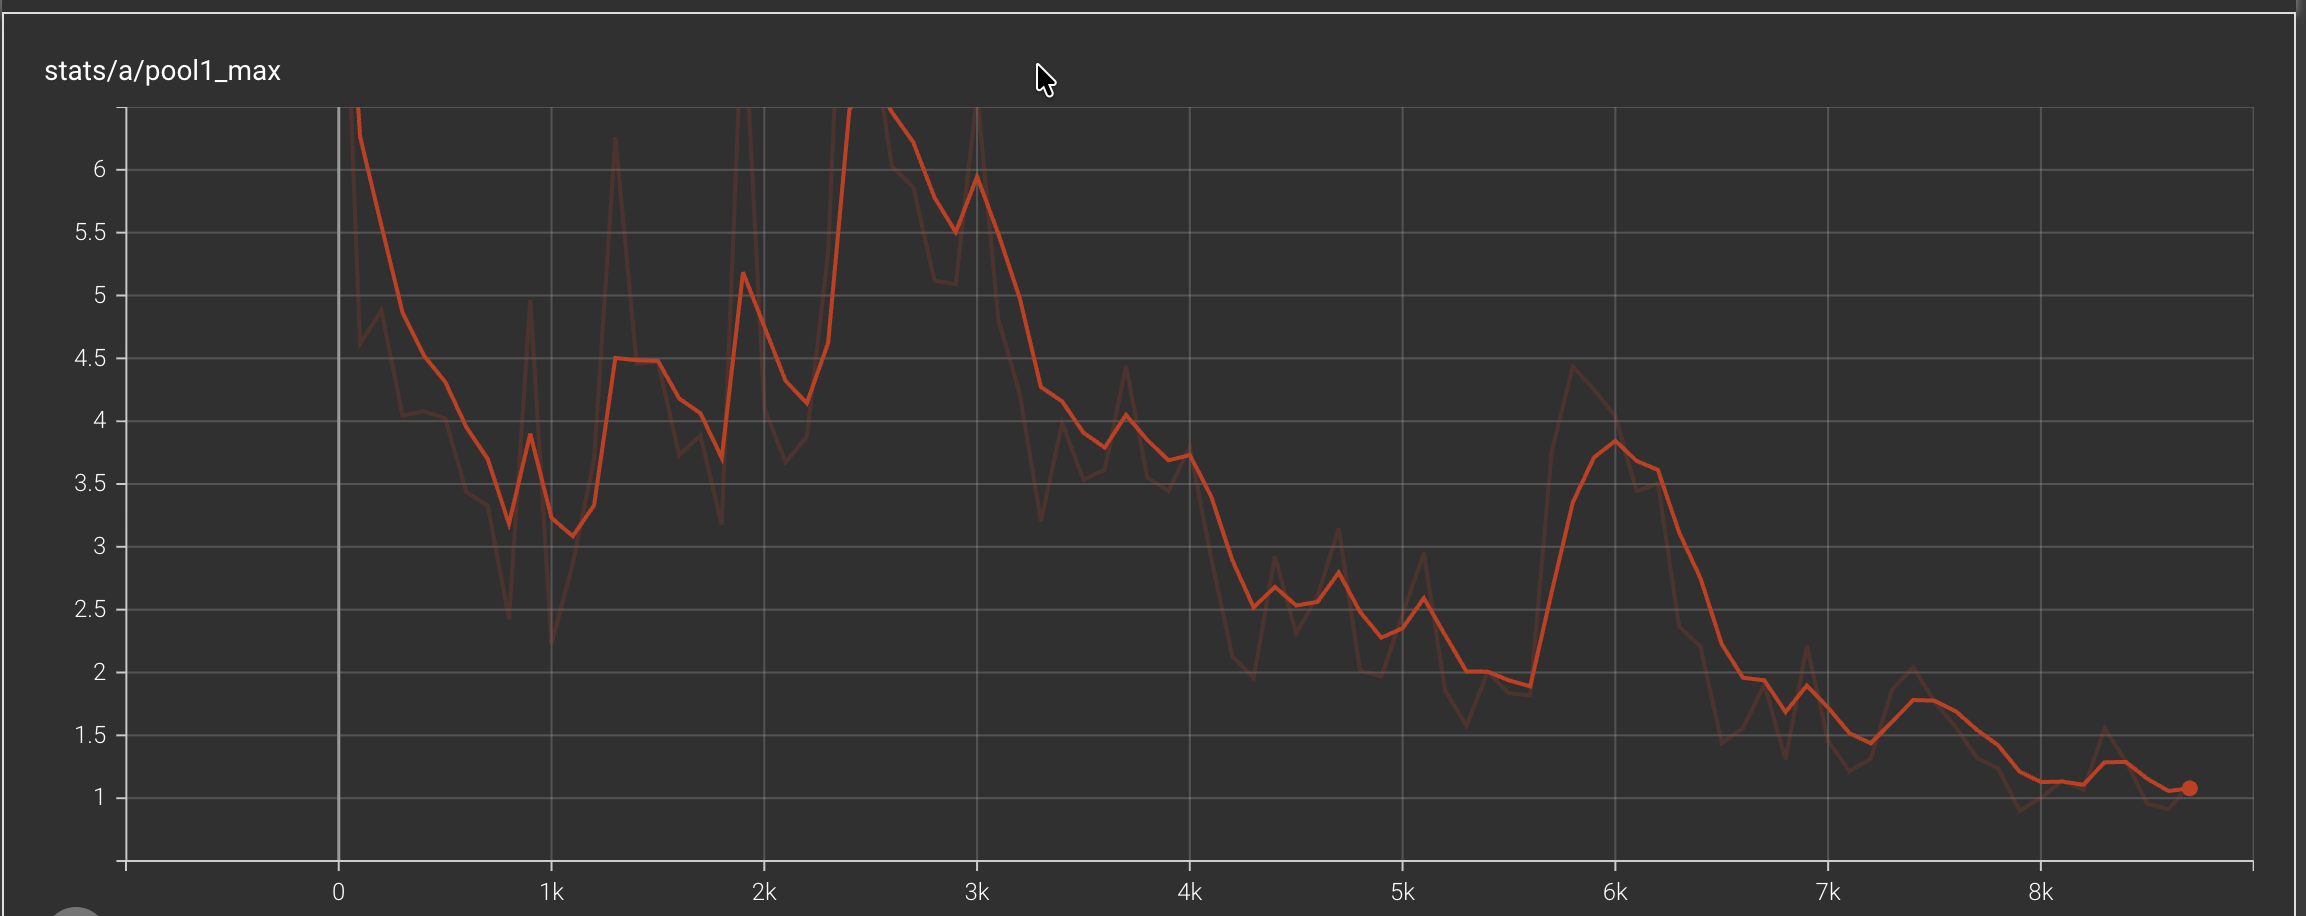
\includegraphics[width=.20\linewidth]{figs/tb_stats_a_pool1_max.png}} &
\fbox{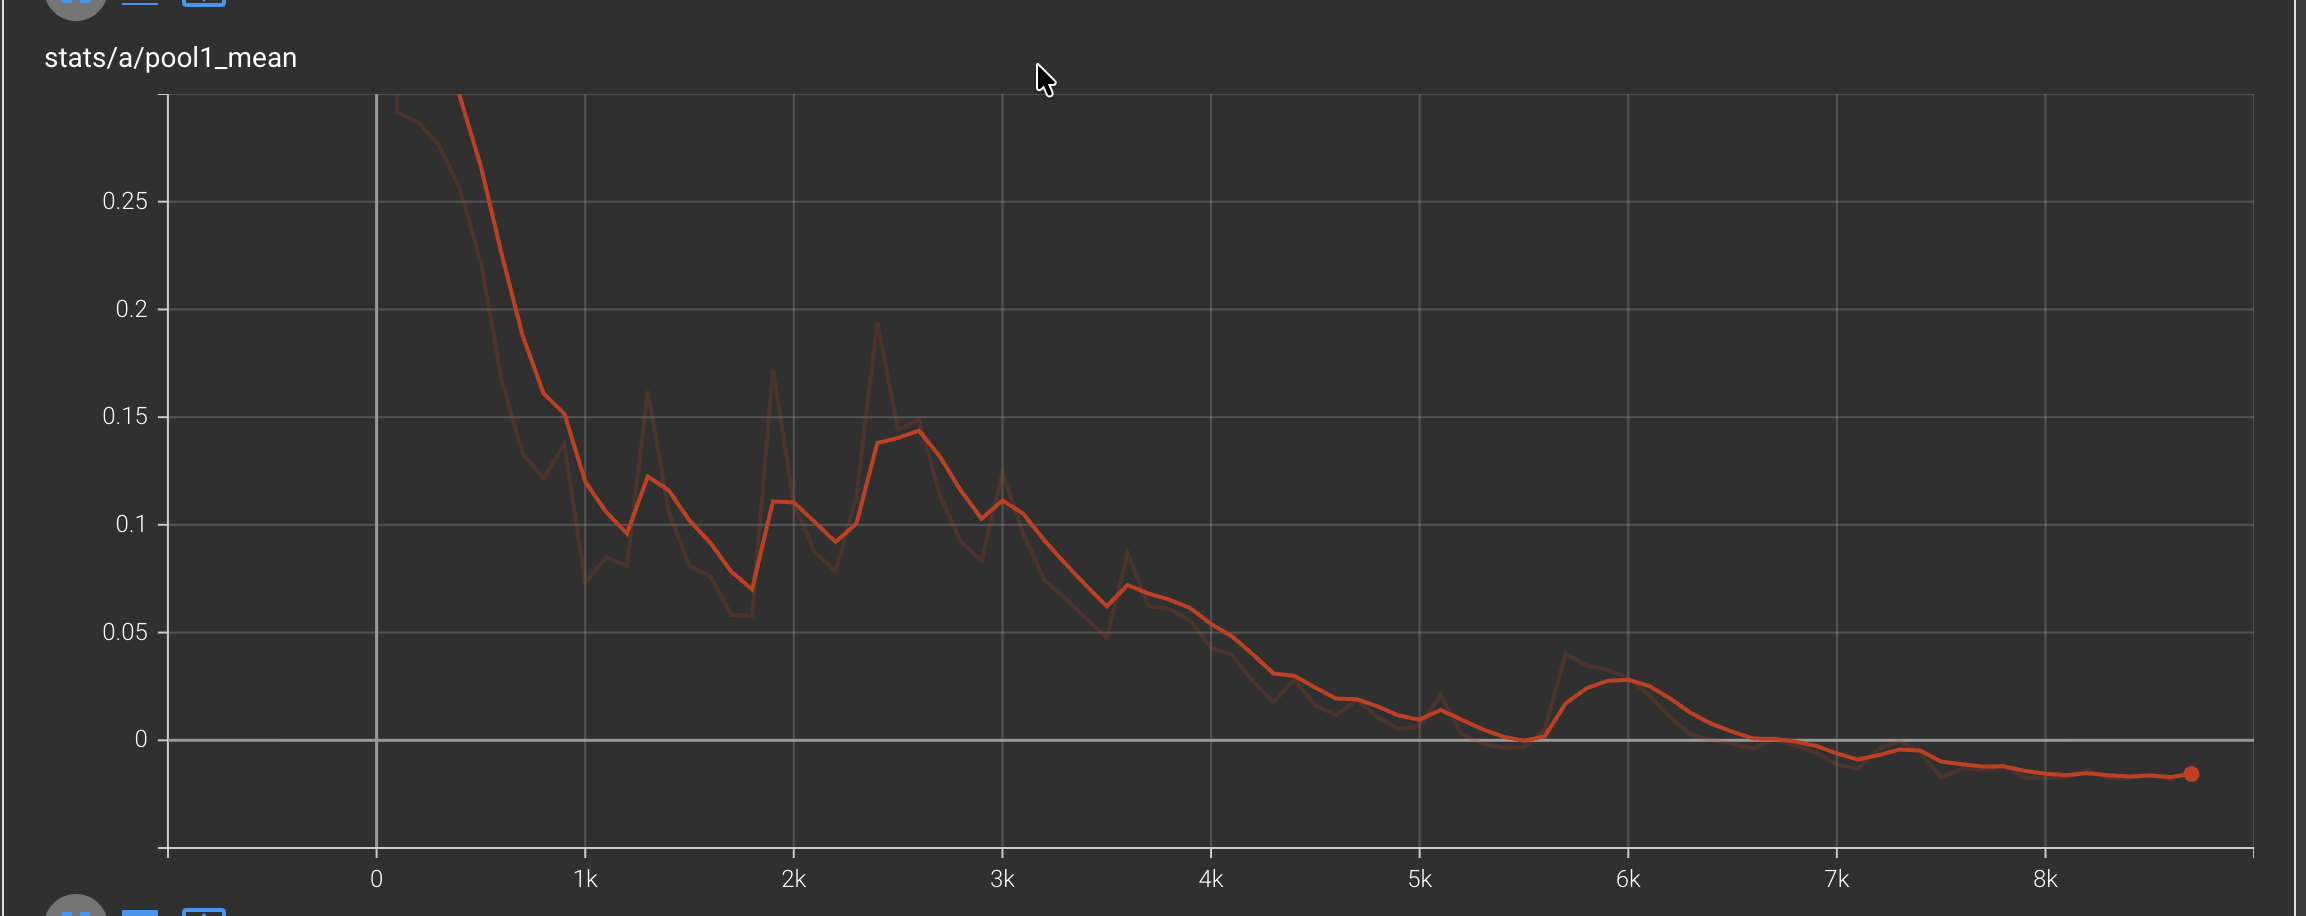
\includegraphics[width=.20\linewidth]{figs/tb_stats_a_pool1_mean.png}} &
\fbox{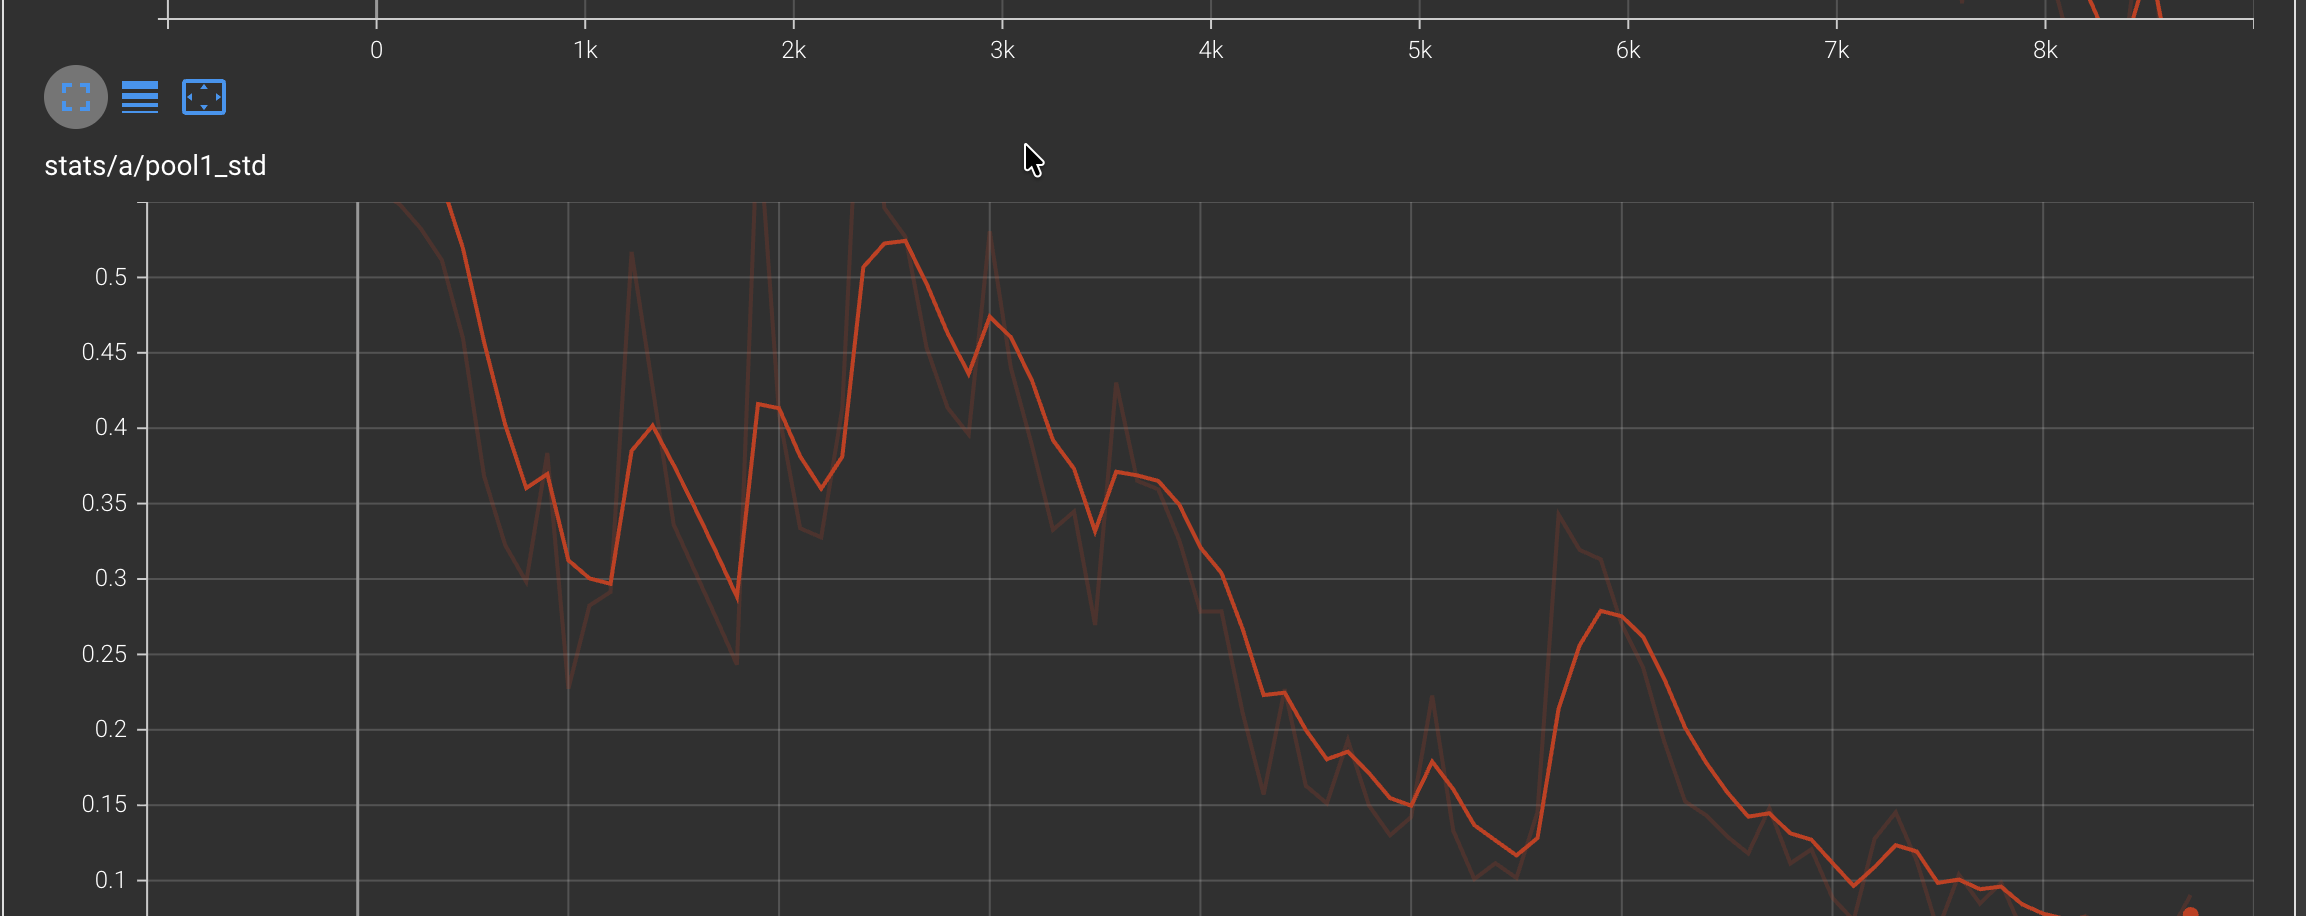
\includegraphics[width=.20\linewidth]{figs/tb_stats_a_pool1_std.png}}\\
Post-MaxPool min & Post-MaxPool max & Post-MaxPool mean & Post-MaxPool std
\end{tabular}

\caption{TensorBoard \emph{time-series} (Scalars) for weights, biases, net inputs, post-ReLU, and post-MaxPool (Run A), showing min/max/mean/std across training.}
\end{figure}


\subsection{(c) More Experiments: Activations, Initializations, and Optimizers}
To study the effect of nonlinearity, initialization, and optimizer, I trained the same DCN
(\S2(a)) under five contrasting configurations. All runs used the same data split (55k/5k/10k).
Unless noted, logging was performed every 100 iterations (histograms + min/max/mean/std)
and validation/test accuracy were logged once per epoch ($\approx$1100 iters at batch size 50).

\begin{table}[H]
\centering
\begin{tabular}{@{}lllll@{}}
\toprule
\textbf{Run} & \textbf{Activation} & \textbf{Init} & \textbf{Optimizer (LR)} & \textbf{Batch}\\
\midrule
A & ReLU & Kaiming/He & Adam (1e-3) & 50 \\
B & Tanh & Xavier/Glorot & SGD + Momentum (0.01, $m{=}0.9$) & 50 \\
C & LeakyReLU & Kaiming/He & RMSProp (1e-3, $m{=}0.9$) & 50 \\
D & Sigmoid & Xavier/Glorot & SGD (0.05) & 50 \\
E & ReLU & Kaiming/He & Adagrad (1e-2) & 50 \\
\bottomrule
\end{tabular}
\caption{Five DCN training runs (\S2(c)).}
\end{table}

\paragraph{How to read the figures.}
For each run below I show: (1) the training loss \emph{for that run only} (so its curve shape is
clear without overlays), and (2) a representative histogram from TensorBoard depicting the
distribution of either preactivations ($z$) or activations ($a$) at an early convolutional layer.
Overlaid, cross-run comparisons (loss/val/test curves for all A--E) are shown in \S2(b).

\paragraph{Run A --- ReLU + Kaiming + Adam (baseline).}
Typically fastest and most stable convergence among the tested settings. ReLU promotes sparse
activations; Kaiming init keeps layerwise variances stable for ReLUs; Adam adapts per-parameter
step sizes and handles plateaus well.
\begin{figure}[H]
\centering
\begin{tabular}{cc}
\fbox{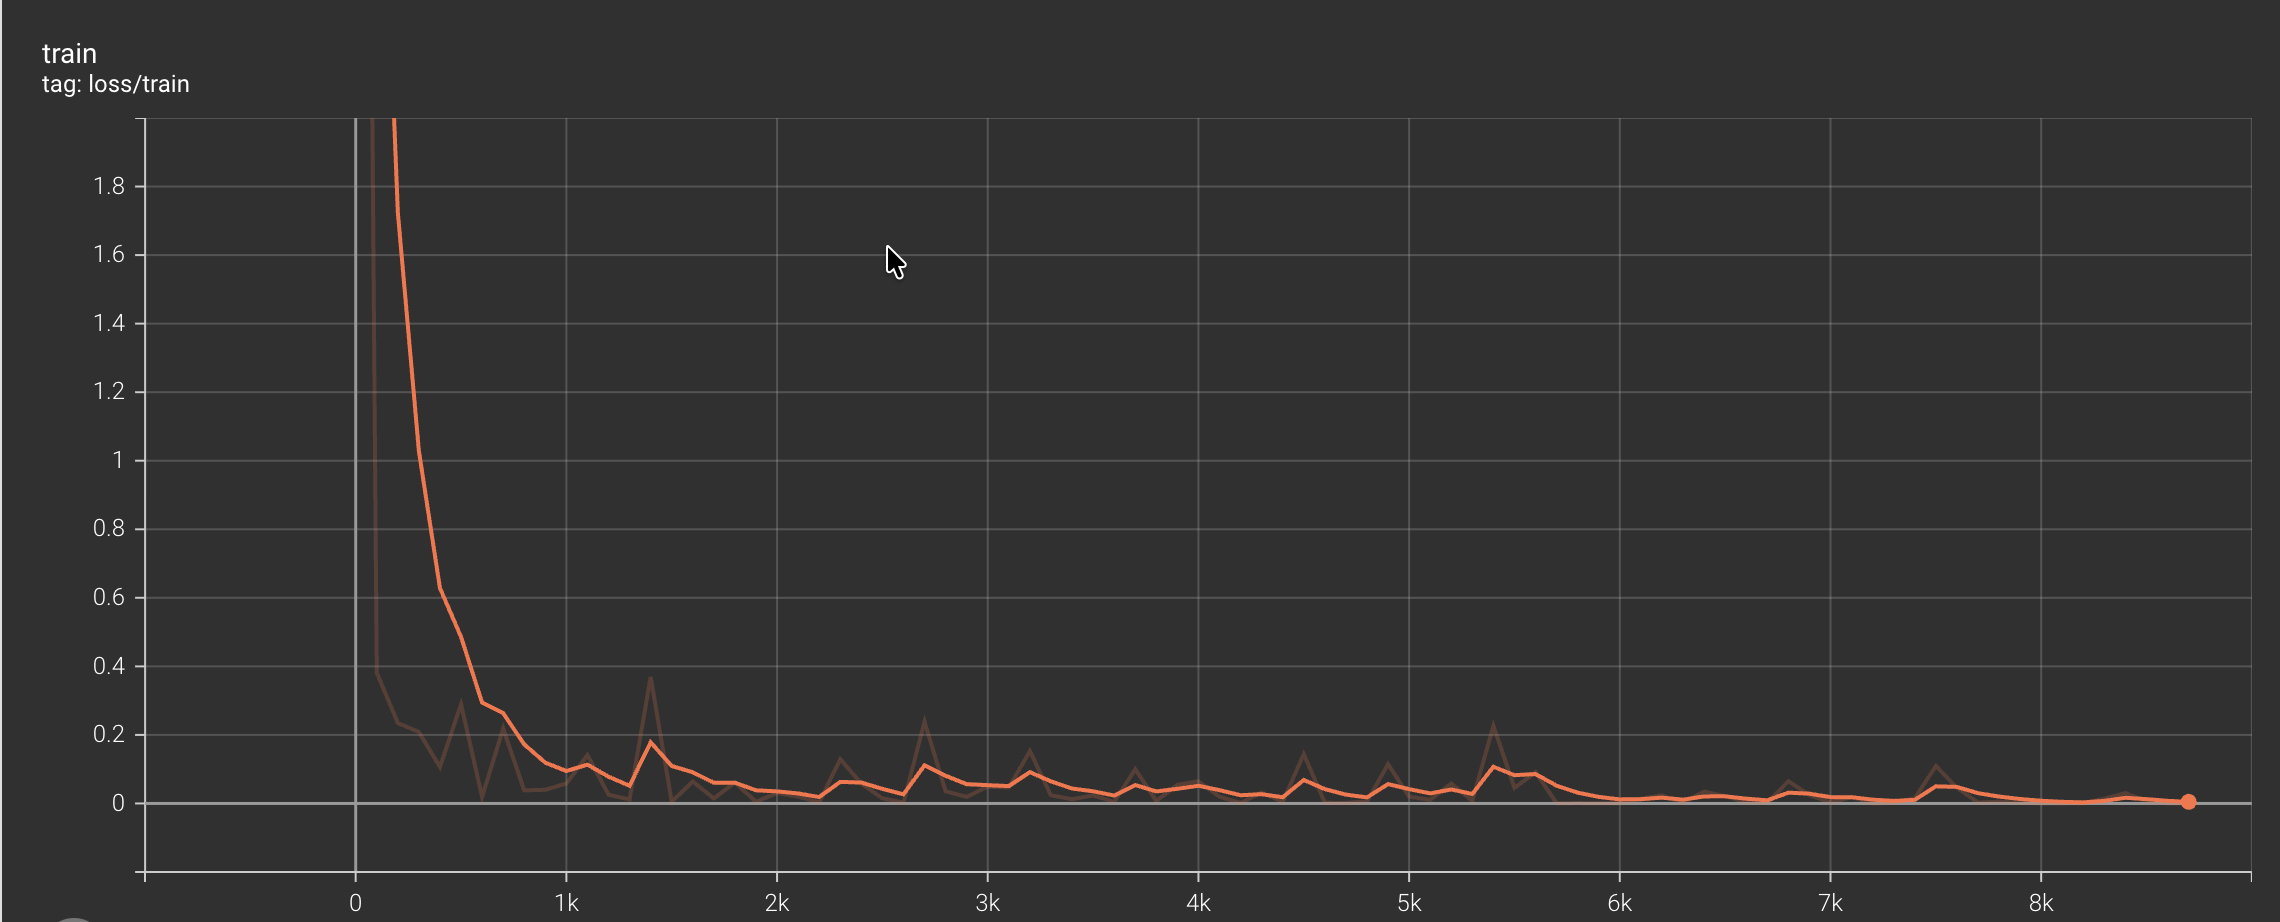
\includegraphics[width=.45\linewidth]{figs/tb_runA_loss.png}} &
\fbox{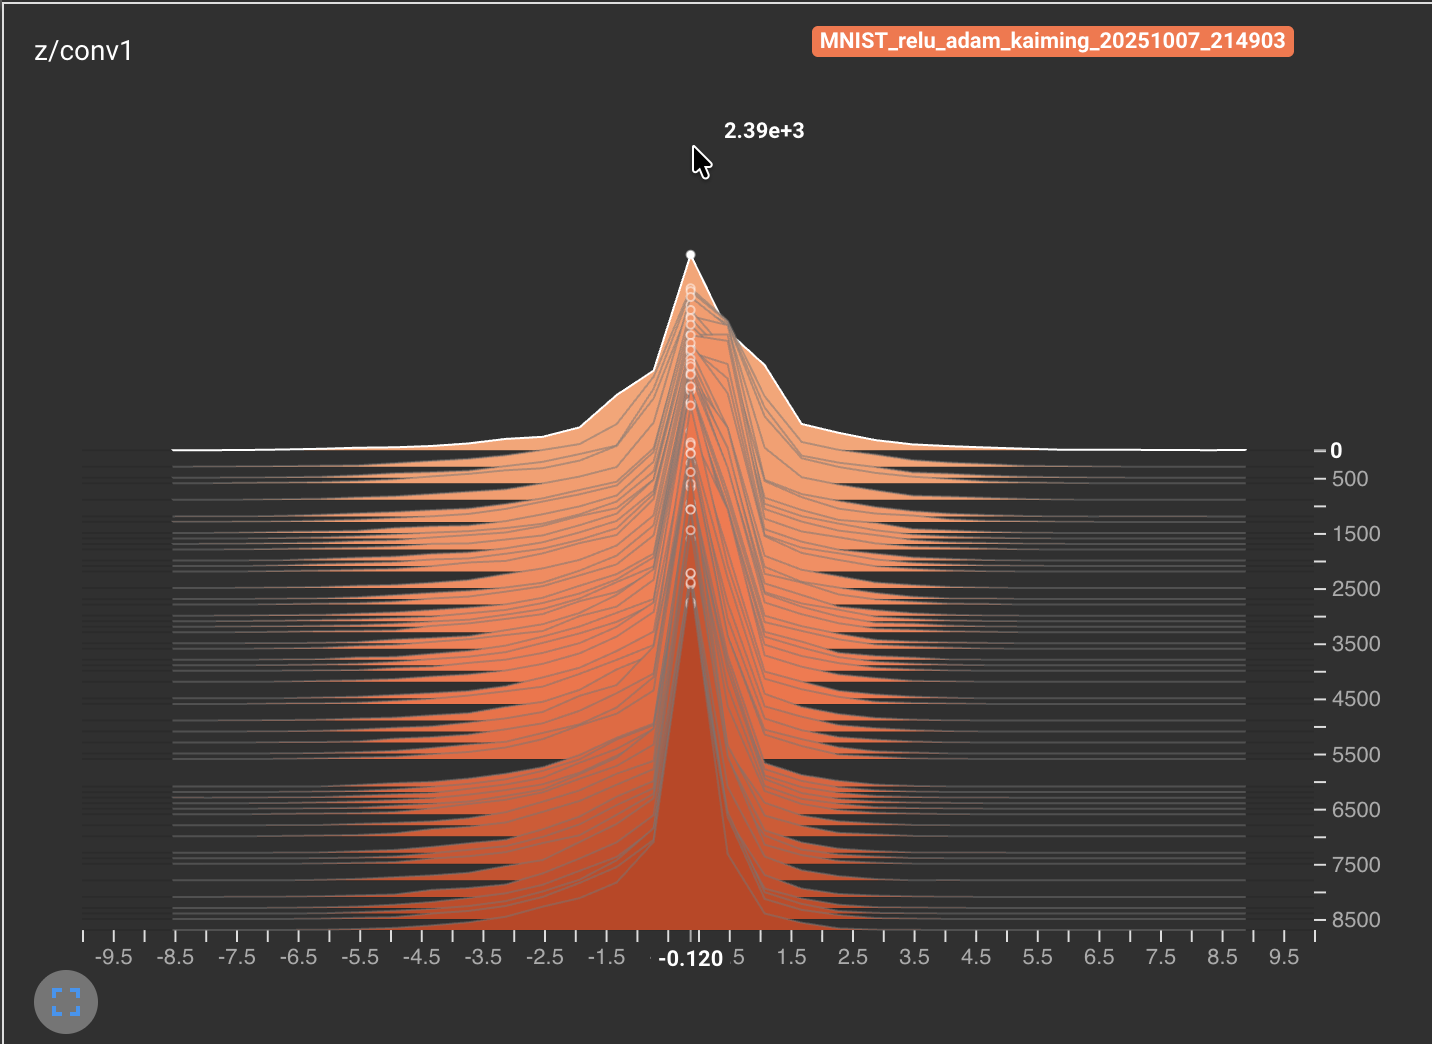
\includegraphics[width=.45\linewidth]{figs/tb_runA_z_conv1_hist.png}}\\
Loss (Run A only) & Preactivations $z$ (conv1) histogram (Run A)
\end{tabular}
\caption{Run A: convergence behavior and $z$-distribution.}
\end{figure}

\paragraph{Run B --- Tanh + Xavier + Momentum SGD.}
Tanh is smooth but can saturate; Xavier maintains variance across layers for symmetric activations.
Momentum helps SGD traverse ravines but may require a slightly higher LR to match Adam's pace.
\begin{figure}[H]
\centering
\begin{tabular}{cc}
\fbox{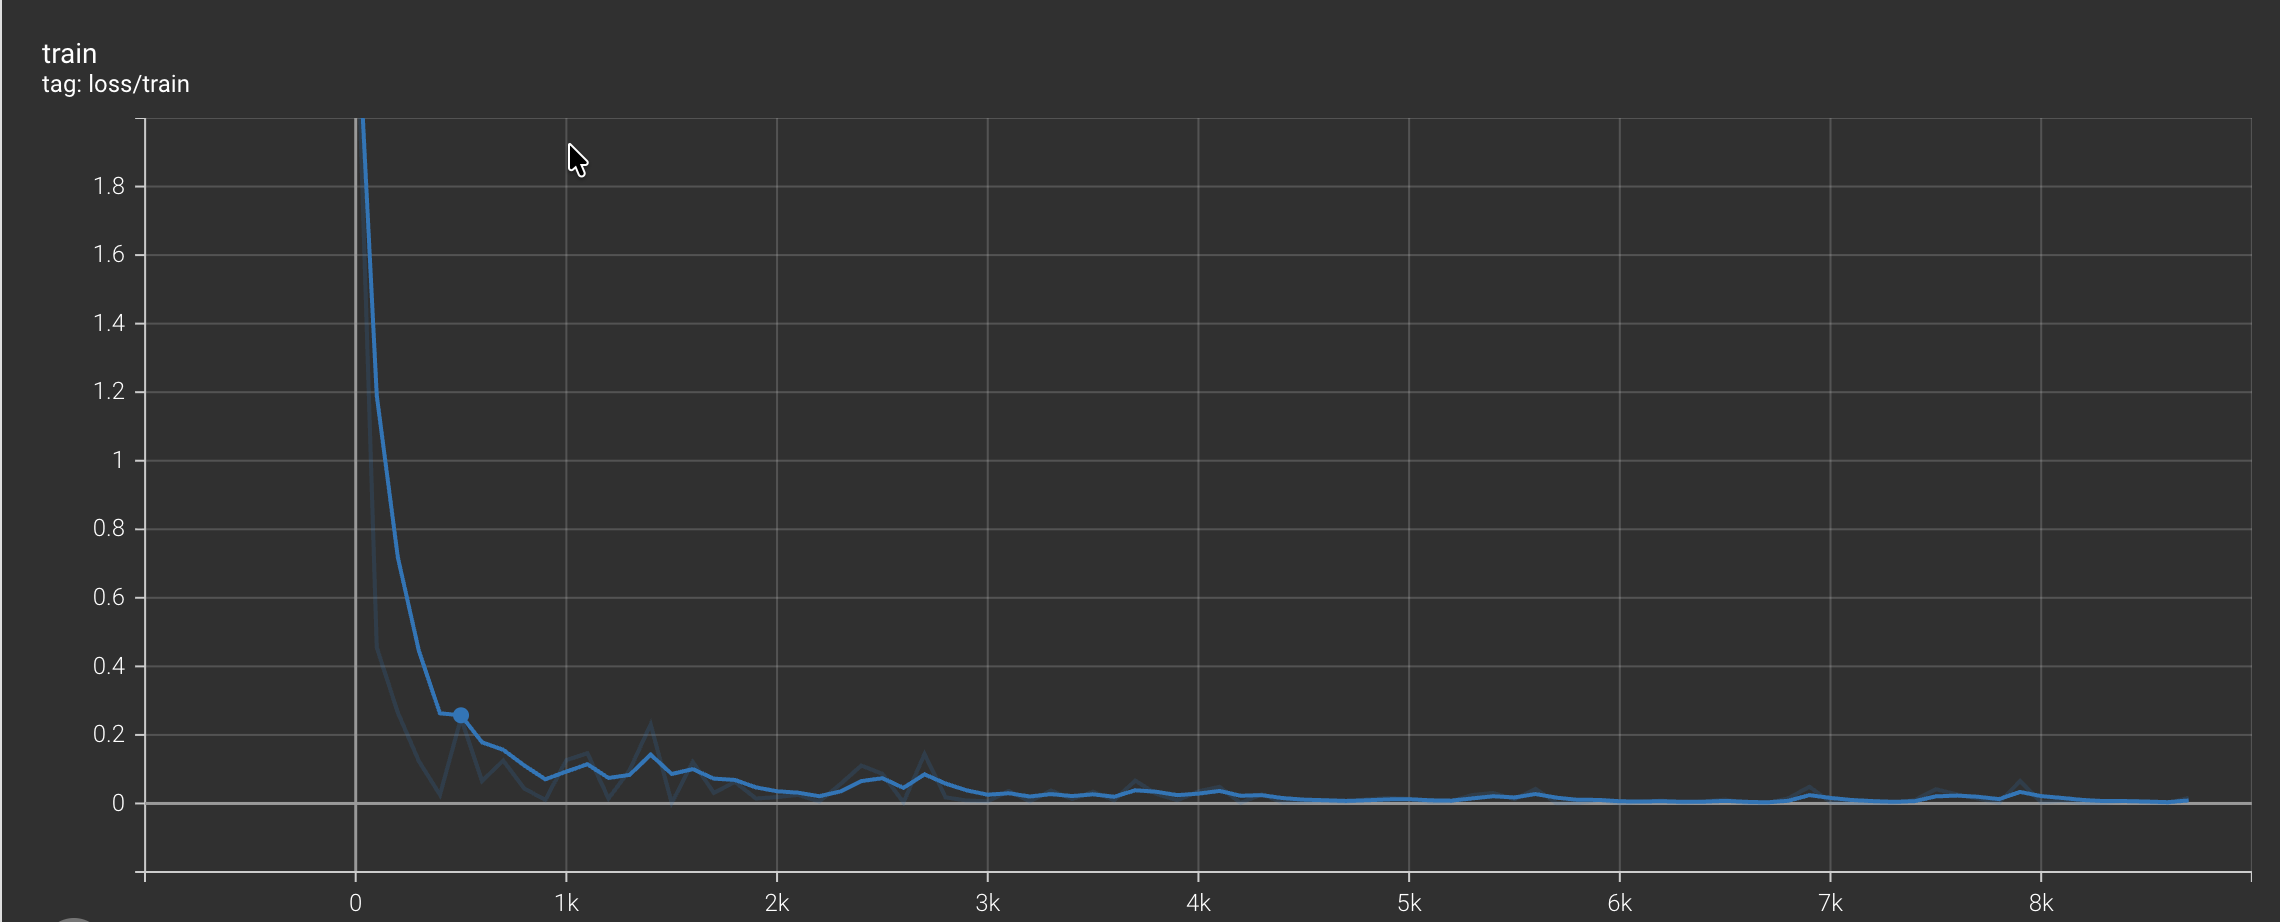
\includegraphics[width=.45\linewidth]{figs/tb_runB_loss.png}} &
\fbox{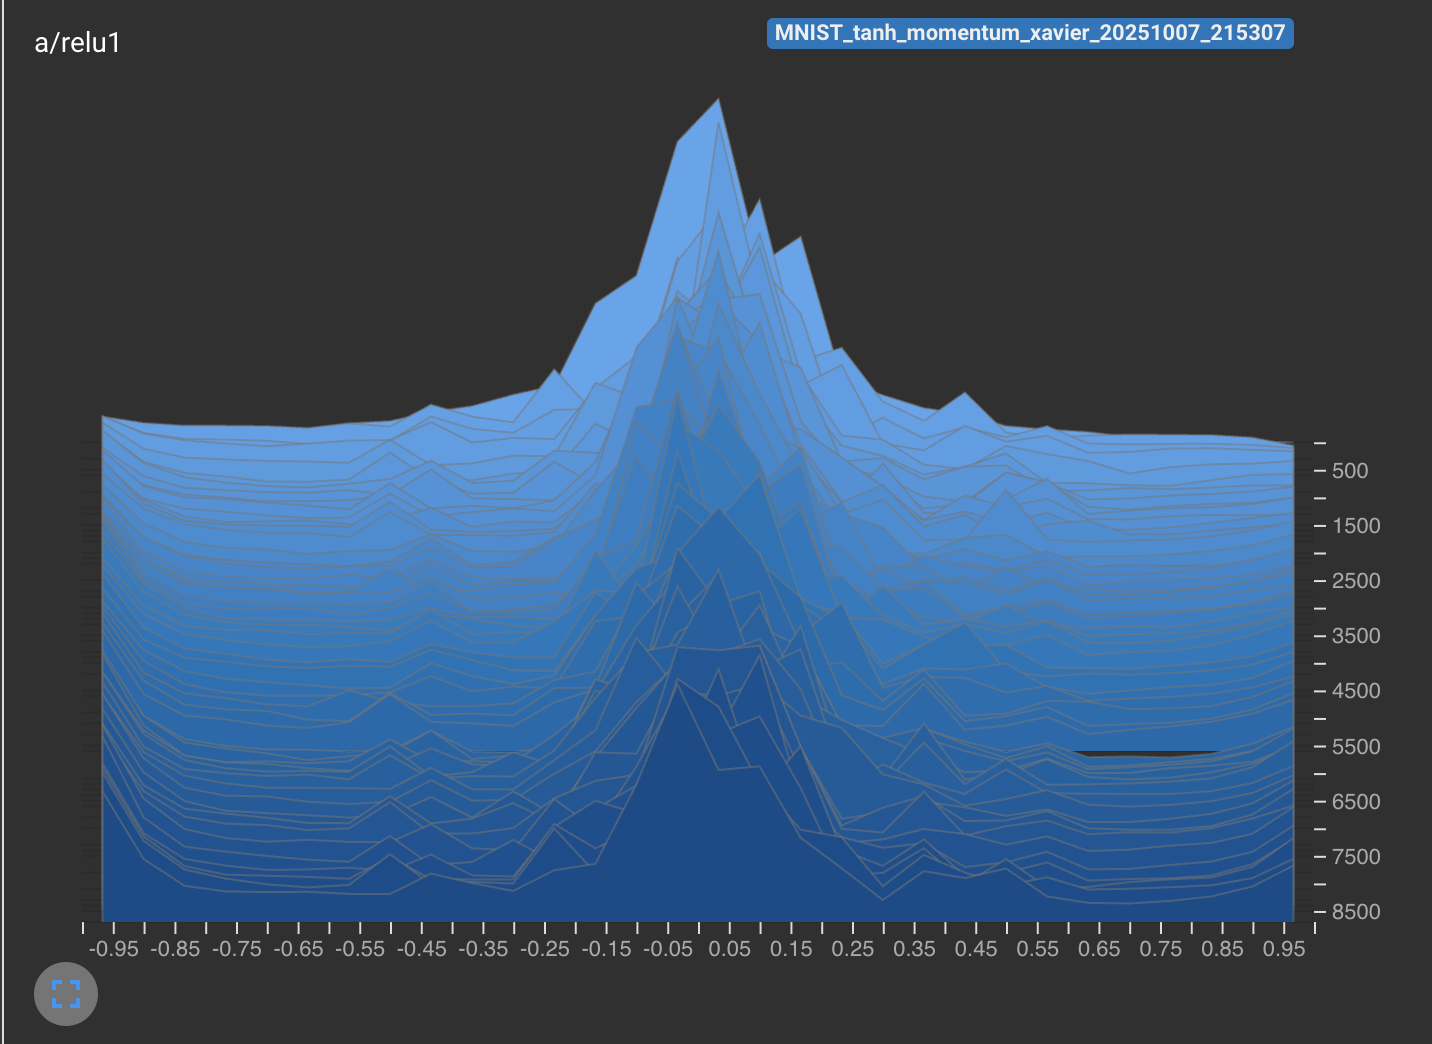
\includegraphics[width=.45\linewidth]{figs/tb_runB_a_relu1_hist.png}}\\
Loss (Run B only) & Activations after ReLU1 (Run B)
\end{tabular}
\caption{Run B: slower start and smoother distributions vs. ReLU.}
\end{figure}

\newpage

\paragraph{Run C --- LeakyReLU + Kaiming + RMSProp.}
LeakyReLU alleviates ``dying ReLU'' by allowing small negative slopes; RMSProp normalizes
by a running RMS of gradients and can be steadier than plain momentum on MNIST.
\begin{figure}[H]
\centering
\begin{tabular}{cc}
\fbox{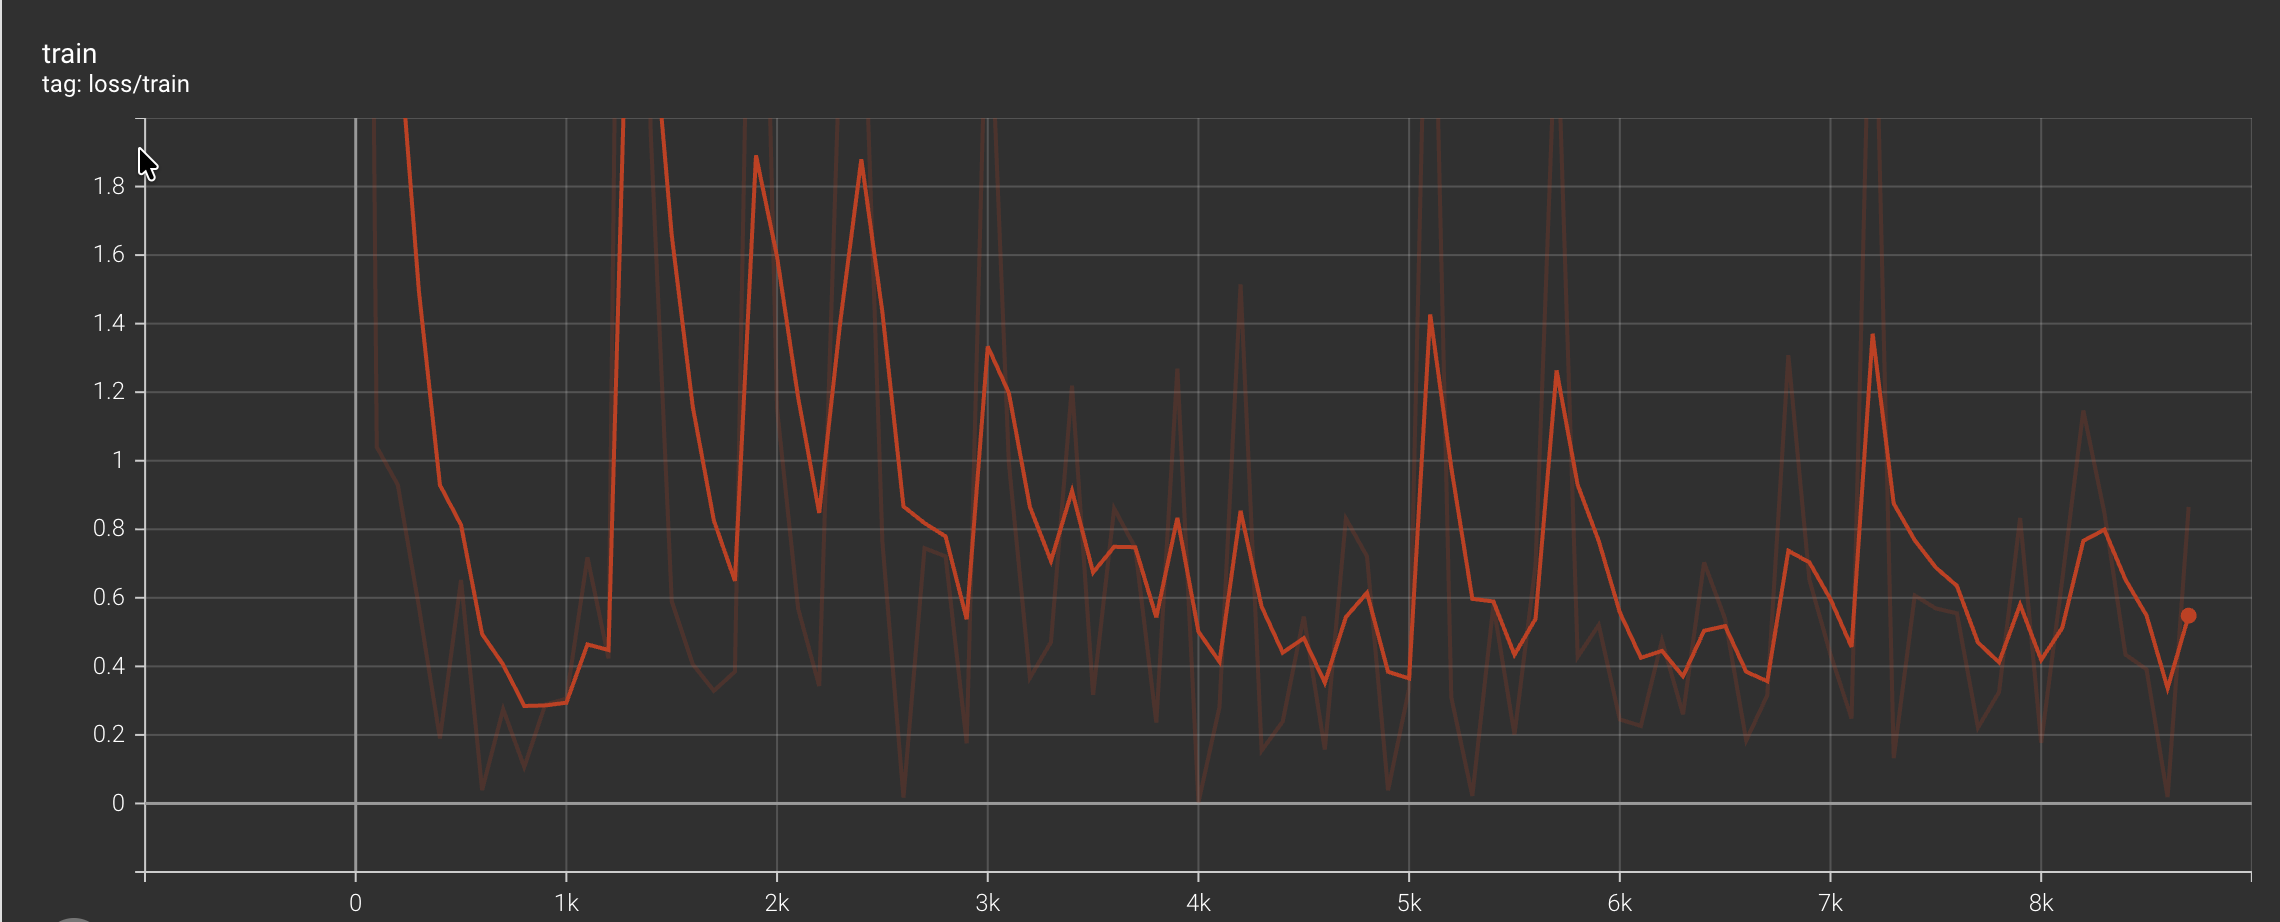
\includegraphics[width=.45\linewidth]{figs/tb_runC_loss.png}} &
\fbox{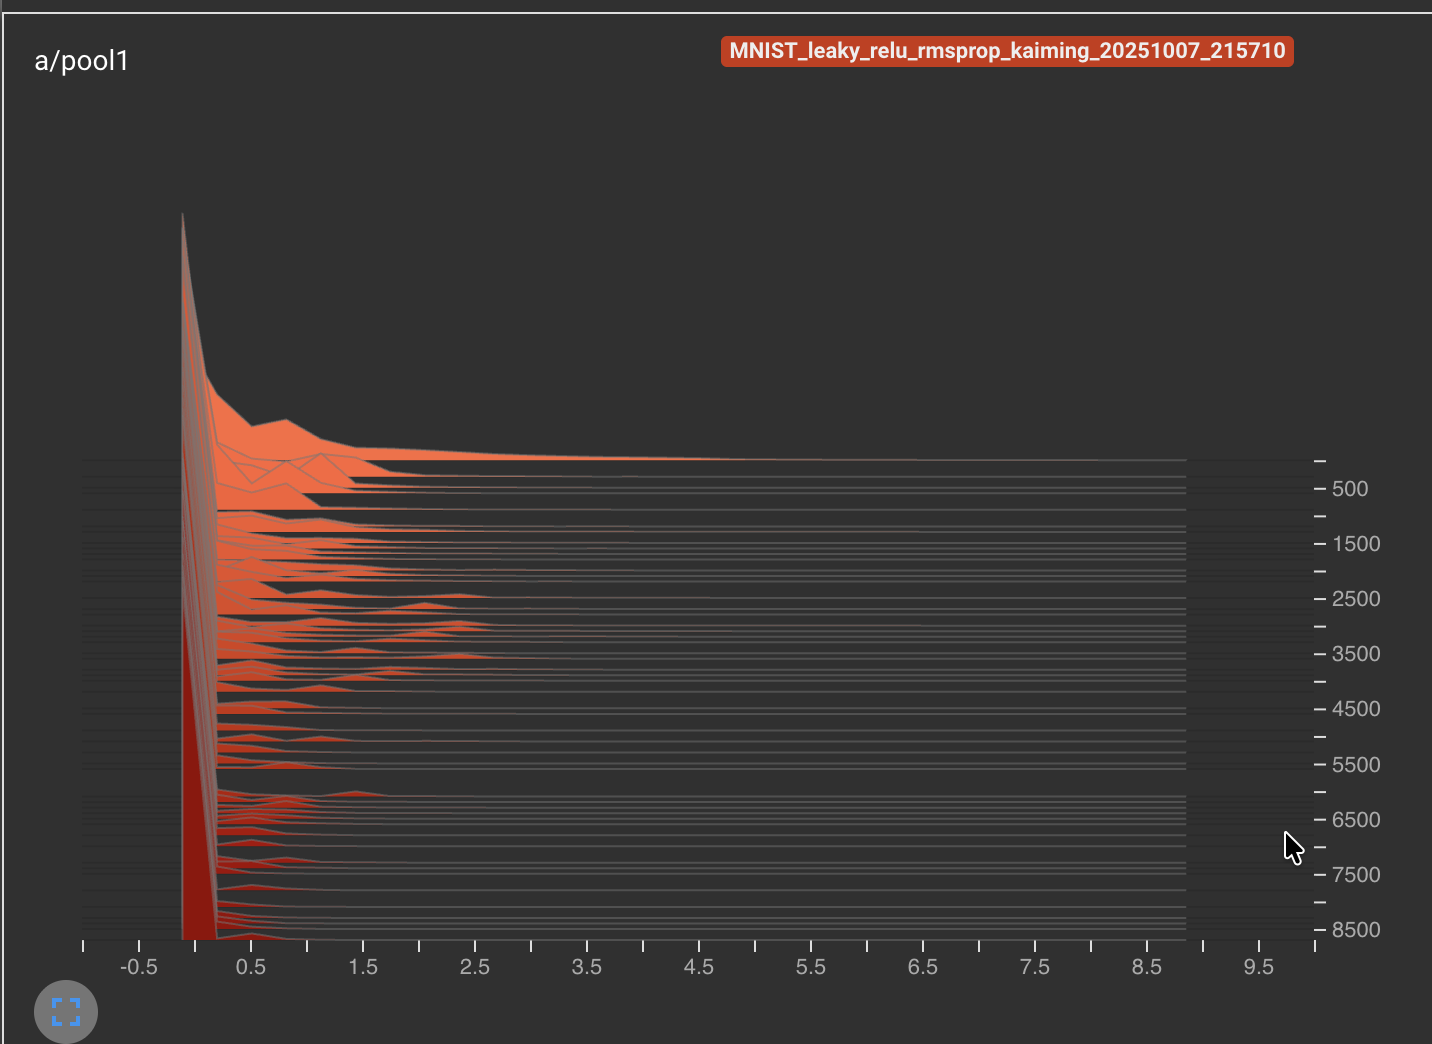
\includegraphics[width=.45\linewidth]{figs/tb_runC_a_pool1_hist.png}}\\
Loss (Run C only) & Post-MaxPool activations histogram (Run C)
\end{tabular}
\caption{Run C: stable training and nonzero mass in the negative preactivation range before LeakyReLU.}
\end{figure}


\paragraph{Run D --- Sigmoid + Xavier + SGD.}
Sigmoid saturates for large $|z|$, yielding smaller gradients and slower progress; Xavier init helps
but early layers may still show narrower dynamic ranges. This run highlights saturation effects.
\begin{figure}[H]
\centering
\begin{tabular}{cc}
\fbox{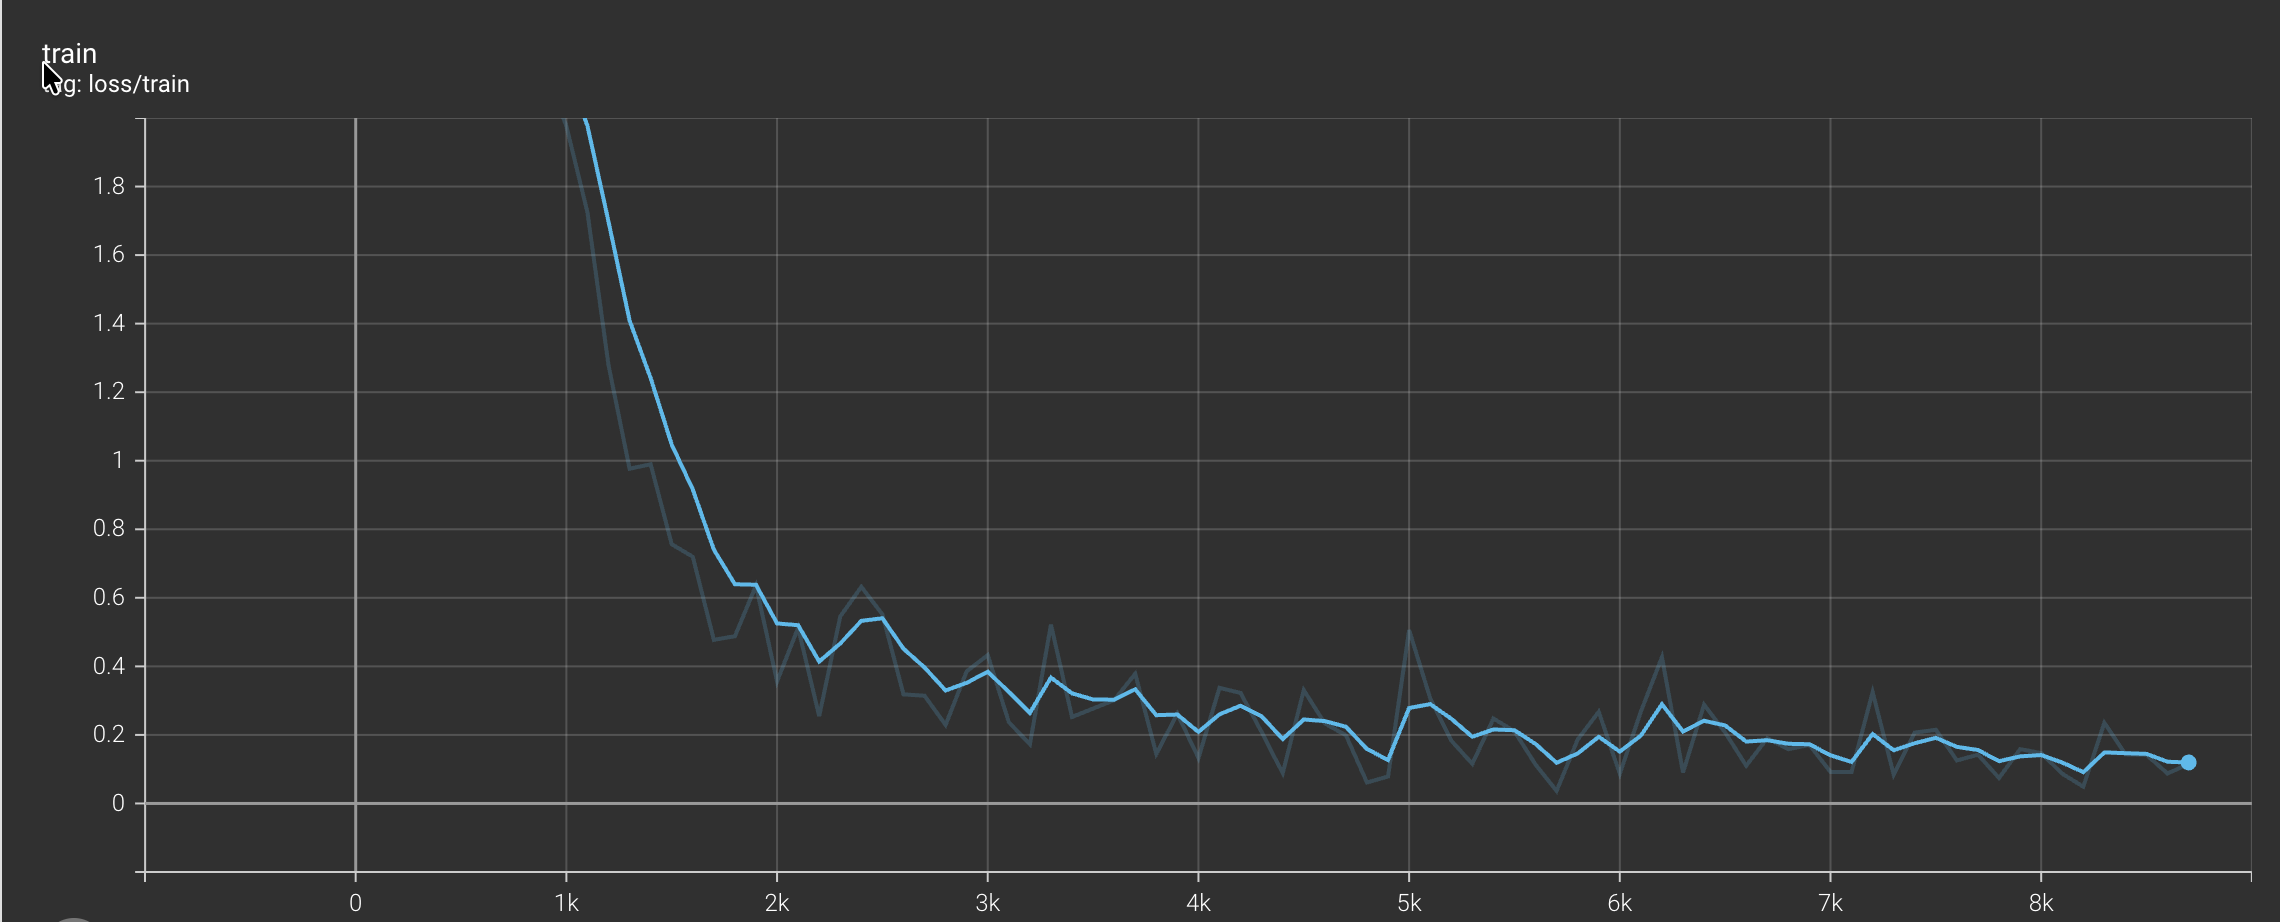
\includegraphics[width=.45\linewidth]{figs/tb_runD_loss.png}} &
\fbox{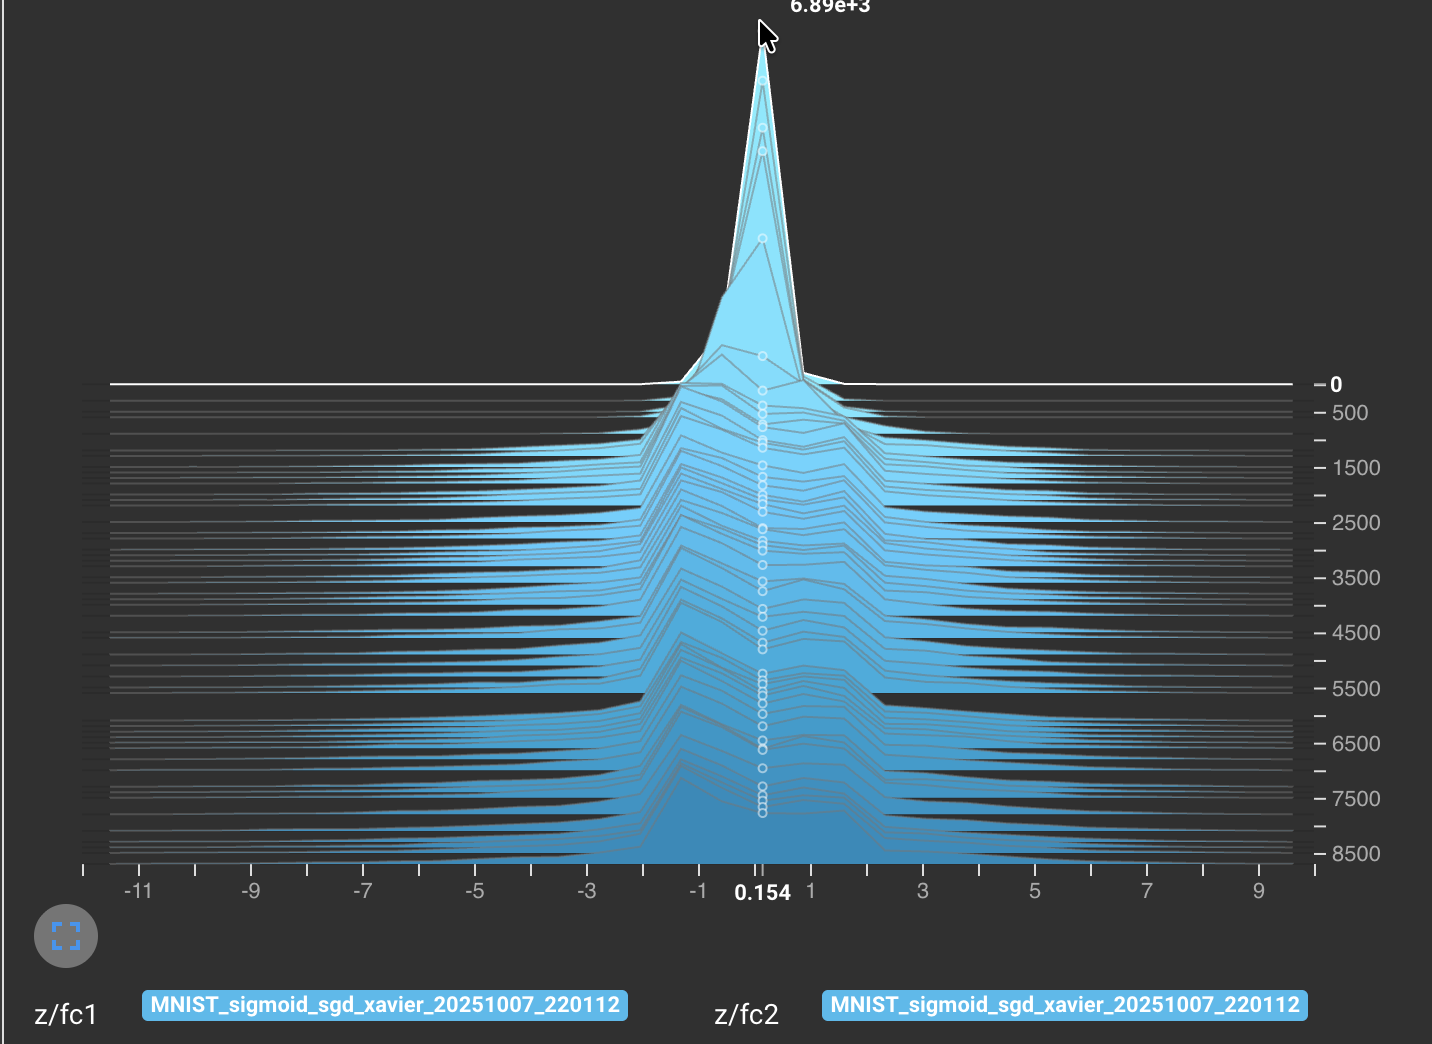
\includegraphics[width=.45\linewidth]{figs/tb_runD_z_conv1_hist.png}}\\
Loss (Run D only) & Preactivations $z$ (conv1) histogram (Run D)
\end{tabular}
\caption{Run D: slower descent and more concentrated $z$ distribution (saturation).}
\end{figure}

\newpage

\paragraph{Run E --- ReLU + Kaiming + Adagrad.}
Adagrad makes aggressive early progress but can decay its effective step size, sometimes plateauing.
Good to contrast with Adam to see different late-epoch behavior.
\begin{figure}[H]
\centering
\begin{tabular}{cc}
\fbox{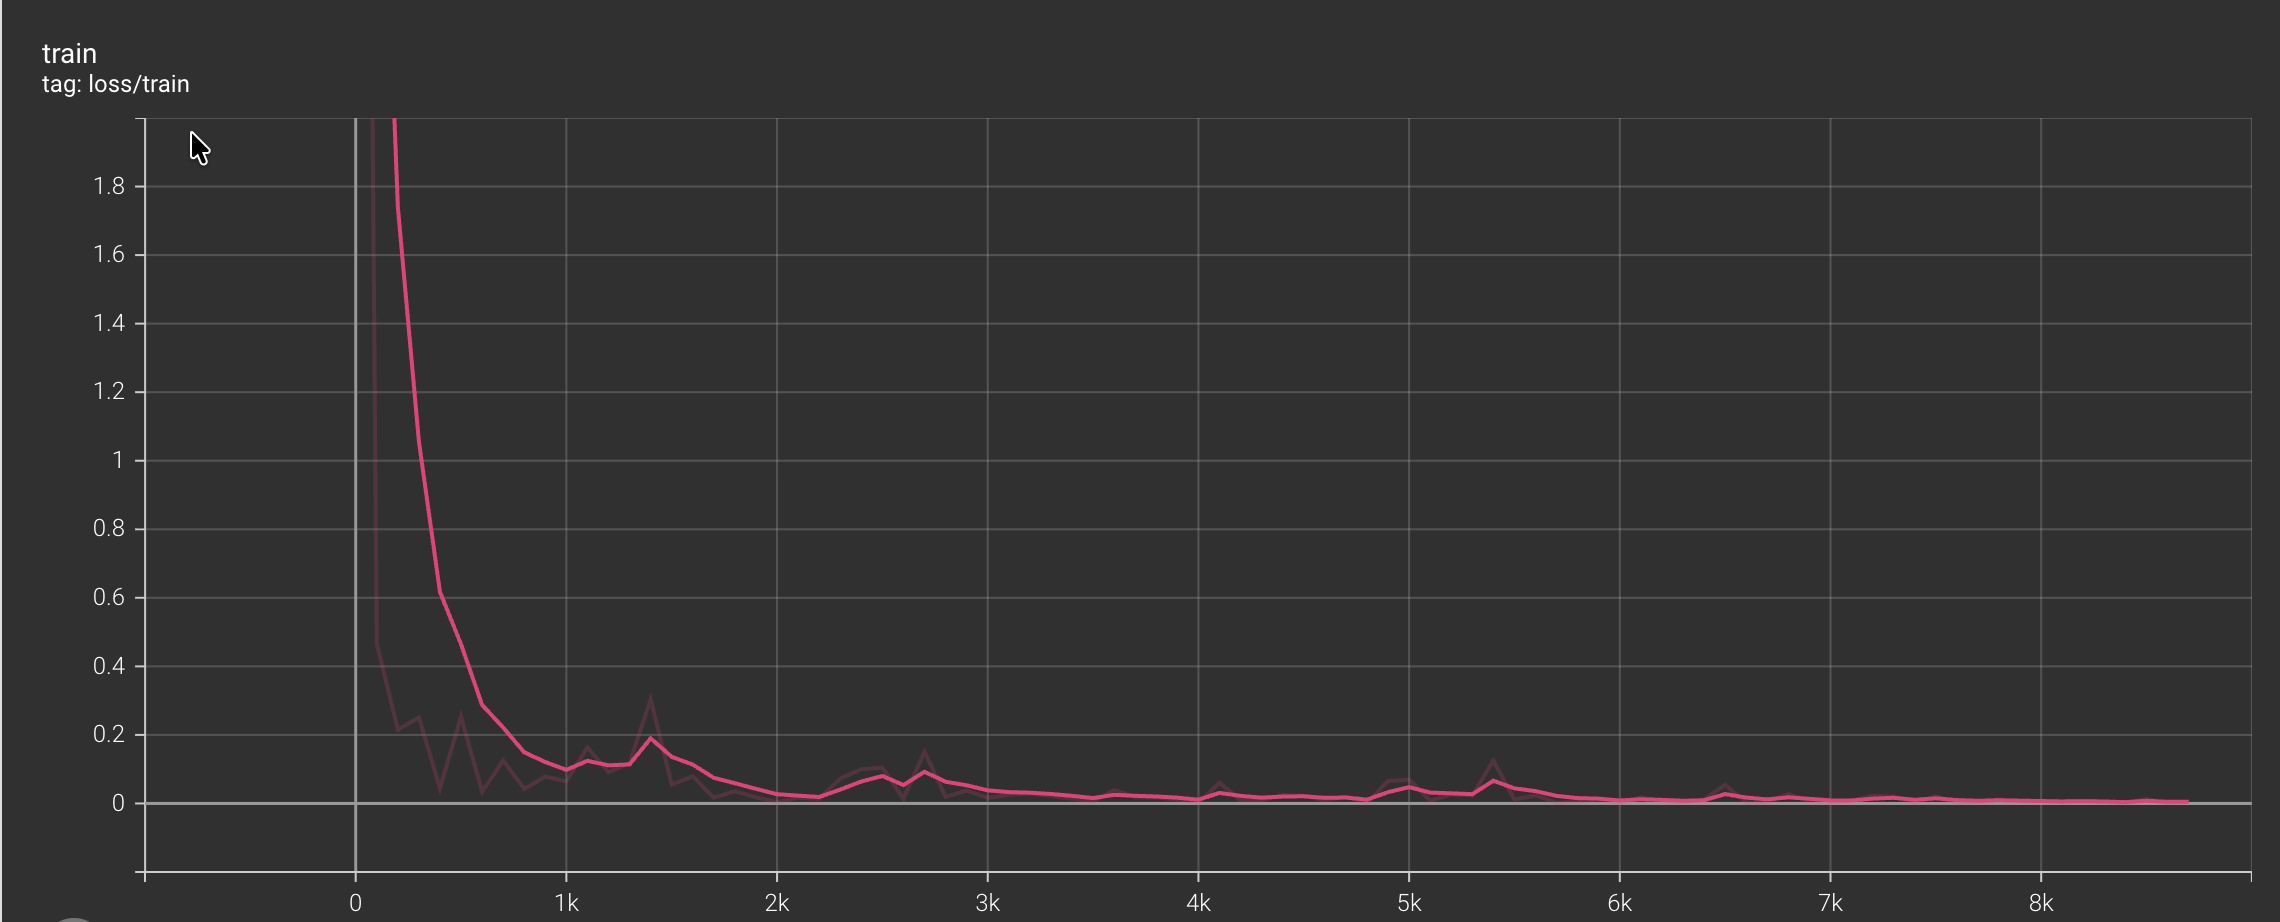
\includegraphics[width=.45\linewidth]{figs/tb_runE_loss.png}} &
\fbox{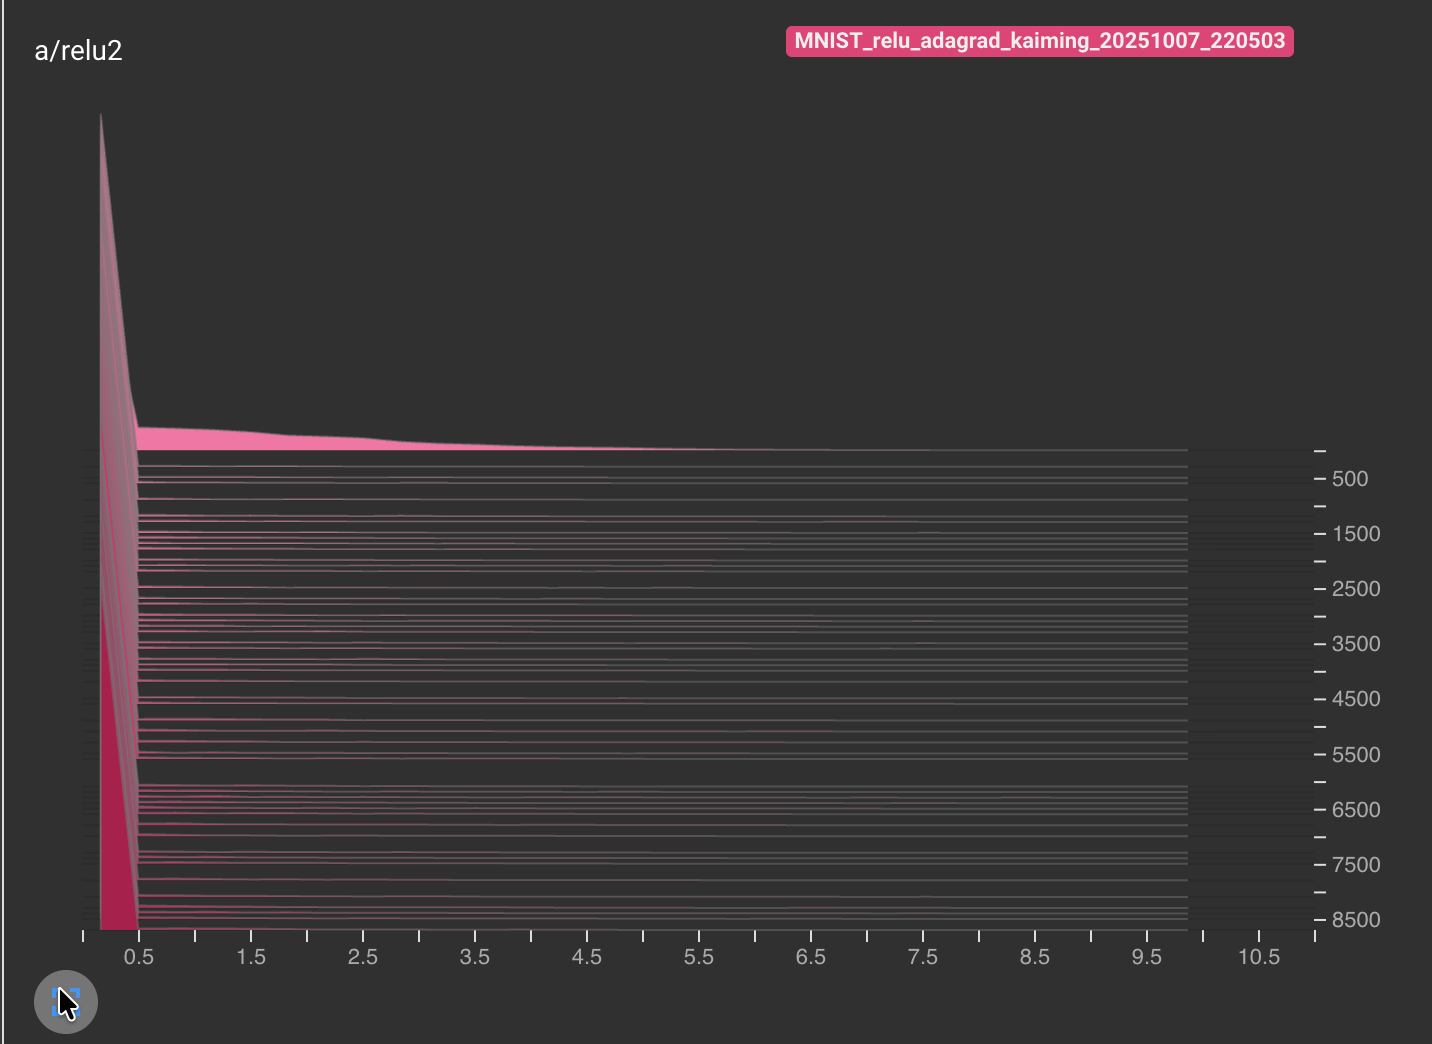
\includegraphics[width=.45\linewidth]{figs/tb_runE_a_relu2_hist.png}}\\
Loss (Run E only) & Activations after ReLU2 histogram (Run E)
\end{tabular}
\caption{Run E: strong early improvement; potential late-epoch plateau.}
\end{figure}


\paragraph{Observations.}
\begin{itemize}[leftmargin=1.2em]
  \item \textbf{Run A (ReLU+Kaiming+Adam):} fastest, most stable training; high final accuracy.
  \item \textbf{Run B (Tanh+Xavier+Momentum):} smooth but slightly slower early training; best final test accuracy.
  \item \textbf{Run C (LeakyReLU+Kaiming+RMSProp):} suboptimal with chosen LR/momentum; lower plateaus.
  \item \textbf{Run D (Sigmoid+Xavier+SGD):} noticeable saturation; steady but slower gains.
  \item \textbf{Run E (ReLU+Kaiming+Adagrad):} aggressive early progress; small late-epoch plateau vs. Adam.
\end{itemize}


\begin{table}[H]
\centering
\small
\begin{tabular}{@{}l l l l r r r r@{}}
\toprule
\textbf{Run} & \textbf{Activation} & \textbf{Init} & \textbf{Optimizer} & \textbf{LR} & \textbf{Mom} & \textbf{Best Val Acc} & \textbf{Final Test Acc} \\
\midrule
A & ReLU        & Kaiming & Adam     & 0.001 & --   & 0.9882 & 0.9888 \\
B & Tanh        & Xavier  & Momentum & 0.010 & 0.9  & 0.9882 & \textbf{0.9908} \\
C & LeakyReLU   & Kaiming & RMSProp  & 0.001 & 0.9  & 0.9634 & 0.9548 \\
D & Sigmoid     & Xavier  & SGD      & 0.050 & --   & 0.9612 & 0.9674 \\
E & ReLU        & Kaiming & Adagrad  & 0.010 & --   & 0.9876 & 0.9906 \\
\bottomrule
\end{tabular}
\caption{MNIST DCN results over five runs (batch size $50$, 8 epochs). “Best Val Acc” is the highest validation accuracy reported at epoch end; “Final Test Acc” is the test accuracy at the end of epoch 8.}
\end{table}


\newpage

\section*{Appendix A --- How to generate the figures}
\begin{enumerate}[leftmargin=1.2em]
  \item \textbf{Install dependencies:}
\begin{verbatim}
pip install numpy matplotlib scikit-learn torch torchvision tensorboard
\end{verbatim}
  \item \textbf{Part 1 (Make-Moons):}
\begin{verbatim}
python code/three_layer_neural_network.py
python code/n_layer_neural_network.py
\end{verbatim}
  Figures will be saved under \texttt{report/figs/*.png}.
  \item \textbf{Part 2 (MNIST DCN):}
\begin{verbatim}
python code/assignment_1_pytorch_mnist_skeleton-1.py --epochs 8 --optimizer adam \
  --activation relu --init kaiming --batch-size 128
tensorboard --logdir runs
\end{verbatim}
\end{enumerate}

\section*{Appendix B --- Notes on implementation details}
\begin{itemize}[leftmargin=1.2em]
  \item For softmax, I subtract the row-wise max before exponentiation for numerical stability.
  \item In the deeper net, L2 regularization adds \( \frac{\lambda}{2}\sum_\ell \|W^\ell\|_2^2 \) to the loss and \( \lambda W^\ell \) to \( \partial \mathcal{L}/\partial W^\ell \).
  \item All toy-network plots are created with a common helper that evaluates \(\hat{y}=\arg\max\) on a grid and contours the classes.
\end{itemize}

\small

\section*{AI Assistance Declaration}
\noindent I used AI tools (ChatGPT) only for language editing—grammar, phrasing, formatting, and document structuring. No AI tools were used to write, debug, or generate any code, nor to design experiments, implement algorithms, train models, or analyze results. All code and experimentation are my own work.

\normalsize
\end{document}
